\input{/fakepath/head.tex}

\begin{document}

\title{Mathe LK Rh}
\author{Tim D.}
\date{MSS 2017-20}
\maketitle

\tableofcontents
\newpage

\part{11/1}

\chapter{Terme, Gleichungen, Ungleichungen}
\section{Pascalsches Dreieck}
\begin{tabular}{rccccccccccccccccc}
  $n=0$:&    &    &    &    &    &    &    &    &  1\\\noalign{\smallskip\smallskip}
  $n=1$:&    &    &    &    &    &    &    &  1 &    &  1\\\noalign{\smallskip\smallskip}
  $n=2$:&    &    &    &    &    &    &  1 &    &  2 &    &  1\\\noalign{\smallskip\smallskip}
  $n=3$:&    &    &    &    &    &  1 &    &  3 &    &  3 &    &  1\\\noalign{\smallskip\smallskip}
  $n=4$:&    &    &    &    &  1 &    &  4 &    &  6 &    &  4 &    &  1\\\noalign{\smallskip\smallskip}
  $n=5$:&    &    &    &  1 &    &  5 &    & 10 &    & 10 &    &  5 &    &  1\\\noalign{\smallskip\smallskip}
  $n=6$:&    &    &  1 &    &  6 &    & 15 &    & 20 &    & 15 &    &  6 &    &  1\\\noalign{\smallskip\smallskip}
  $n=7$:&    &  1 &    &  7 &    & 21 &    & 35 &    & 35 &    & 21 &    &  7 &    &  1\\\noalign{\smallskip\smallskip}
  $n=8$:&  1 &    &  8 &    & 28 &    & 56 &    & 70 &    & 56 &    & 28 &    &  8 &    &  1\\\noalign{\smallskip\smallskip}
\end{tabular}
\section{pq-Formel}
\begin{gather*}
  x^2 + px + q = 0 \\
  x_{1/2} = -\frac{p}{2} \pm \sqrt{(\frac{p}{2})^2 - q}
\end{gather*}
\section{abc-Formel}
\begin{gather*}
  ax^2 + bx + c = 0 \\
  x_{1/2} = \frac{-b \pm \sqrt{b^2 - 4ac}}{2a}
\end{gather*}
\section{Satz von Vieta}
\begin{gather*}
  0 = x^2 + px + q
\end{gather*}
pq-Formel:
\begin{gather*}
  x_{1/2} = -\frac{p}{2} \pm \sqrt{\smash[b]{\underbrace{(\frac{p}{2})^2 - q}_{\text{Diskriminante*}}}}
\end{gather*}
*Diskriminante:\\
$ > 0 \gap\Rightarrow\gap \text{zwei Lösungen} $ \\
$ = 0 \gap\Rightarrow\gap \text{eine Lösung} $ \\
$ < 0 \gap\Rightarrow\gap \text{keine Lösung} $
\begin{gather*}
  x_1 + x_2 = -\frac{p}{2} + \sqrt{\cdots} - \frac{p}{2} - \sqrt{\cdots} = -p \\
  x_1 \cdot x_2 = (-\frac{p}{2} + \sqrt{\cdots}) (-\frac{p}{2} - \sqrt{\cdots}) = \frac{p^2}{4} - \frac{p^2}{4} + q = q \\\\
  \Rightarrow x_1 + x_2 = -p \gap x_1 \cdot x_2 = q \\\\
  0 = x^2 + px + q = (x - x_1)(x - x_2) \\
  = x^2 + (-x_1 - x_2)x + x_1 \cdot x_2 \\\\
  \textbf{Beispiel} \\
  \frac{1}{9}x^2 - \frac{2}{3}x - 8 = \frac{1}{9} (x^2 \underbrace{-6}_{x_1 + x_2}x \underbrace{-72}_{x_1 \cdot x_2}) \\
  x_1 = 12; \; x_2 = -6 \\
  0 = \frac{1}{9} \underbrace{(x - 12)(x + 6)}_{\text{Linearfaktoren}}
\end{gather*}
\section{Binomischer Lehrsatz}
\begin{gather*}
  (a + b)^n = \sum_{k=0}^n \binom{n}{k} \cdot a^{n-k} \cdot b^k \\\\
  \textbf{Beispiele} \\
  n = 2 \\
  (a + b)^2 = \underbrace{\sum_{k=0}^2}_{\mathclap{\text{Drei Summanden: k = 0; k = 1; k = 2}}} \binom{2}{k} \cdot a^{2-k} \cdot b^k \\
  = \underbrace{\binom{5}{0}a^2}_{\text{k = 0}} + \underbrace{\binom{5}{1}ab}_{\text{k = 1}} + \underbrace{\binom{5}{2}b^2}_{\text{k = 2}} \\
  = 1 \cdot a^2 + 2 \cdot ab + 1 \cdot b^2 = a^2 + 2ab + b^2 \\\\
  n = 5 \\
  (a + b)^2 = \sum_{k=0}^5 \binom{5}{k} \cdot a^{5-k} \cdot b^k \\
  = \binom{5}{0}a^5 + \binom{5}{1}a^4b^{1} + \binom{5}{2}a^3b^2 + \binom{5}{3}a^2b^3 + \binom{5}{4}a^{1}b^4 + \binom{5}{5}b^5 \\
  = a^5 + 5a^4b + 10a^3b^2 + 10a^2b^3 + 5ab^4 + b^5
\end{gather*}
Binominialkoeffizienten
\begin{gather*}
  \binom{n}{k} = \frac{n!}{k! \cdot (n - k)!}
\end{gather*}
\section{Gleichungen und Ungleichungen}
\subsection{Gleichung lösen durch Substitution}
\textbf{Beispiel} $ 0 = 2x^4 - 3x^2 - 5 $ \\
Lösungsmenge der Gleichung = Menge der Nullstellen (Schnitte mit der x-Achse) der Funktion mit gleichem Funktionsterm \\
\begin{gather*}
  \text{substituiere} \; x^2 = t \\
  0 = 2t^2 - 3t - 5 \\
  t_{1/2} = \frac{3 \pm \sqrt{9 + 40}}{4} = \frac{3 \pm 7}{4} \\
  t_1 = 2.5, \gap t_2 = -1 \\\\
  \text{resubstituiere} \\
  t_1 = x^2 = 2.5 \equ \sqrt{} \\
  \gap x_1 = \sqrt{2.5}; \; x_2 = -\sqrt{2.5} \\
  t_2 = x^2 = -1 \equ \sqrt{} \\
  \gap \text{keine Lösung} \\
  L = \{\sqrt{2.5}; -\sqrt{2.5}\}
\end{gather*}
\section{Potenzen, Wurzeln und Logarithmen}
\subsection{Potenz- und Wurzelgesetze}
\begin{gather*}
  a^x \cdot a^y = a^{x + y} \\
  a^x : a^y = a^{x - y} \\
  a^x \cdot b^x = (ab)^x \\
  a^x : b^x = (\frac{a}{b})^x \\
  (a^x)^y = a^{xy} \\
  a^{-x} = \frac{1}{a^x} \\\\
  \sqrt[x]{a^y} = a^\frac{y}{x} \\
  \sqrt[x]{a} \cdot \sqrt[x]{b} = \sqrt[x]{ab} \\
  \sqrt[x]{\sqrt[y]{a}} = \sqrt[xy]{a}
\end{gather*}
\subsection{Logarithmengesetze}
\begin{gather*}
  \log_a(xy) = \log_a(x) + \log_a(y) \\
  \log_a(x^y) = \log_a(x) \cdot y \\
  a^x = 10^{\log(a) \cdot x} \\
  \log_a(x) = \frac{\log(x)}{\log(a)}
\end{gather*}

\chapter{Funktion - Relation - Zahlenfolge}
Eine Funktion ist eine Zuordnung (Zahlen $x \rightarrow$ Zahlen $y$), die jeder Zahl $x$ der Definitionsmenge genau eine Zahl $y$ der Wertemenge zuordnet. \\\\
Darstellung:
\begin{itemize}
  \item Funktionsgleichung, z. B. $f(x) = y = \underbrace{2x^2 + 5}_\text{Funktionsterm}$
  \item Graph
  \item Wertetabelle
\end{itemize}
Eine Relation ist eine allgemeine Zuordnung von $x$ zu $y$,\\
z. B. $x = 3$ (senkrechte Gerade), $x^2y = y^2 + x^3$ \\\\
Eine Zahlenfolge ist eine Funktion mit $x \in \mathbb{N}$
\section{Zahlenfolgen}
Definitionsmenge $D = \mathbb{N}_0$ \\
Wertemenge $W = \mathbb{R}$ \\
$a_n = y = \dots \;\leftarrow Funktionsterm$ \\
Angabe eines Funktionsterms für alle Zahlen nennt man explizite Darstellung der Zahlenfolge. \\
\begin{gather*}
  a_n = (\frac{1}{2})^n \\
  a_1 = \frac{1}{2};\gap a_2 = \frac{1}{4};\gap a_3 = \frac{1}{8}; \gap\dots;\gap a_{100} = 2^{-100}
\end{gather*}
Berechnung der Folgezahlen Schritt für Schritt nennt man implizite Darsteluung der Zahlenfolge. (Rekursion) \\
\begin{gather*}
  a_n = 2 \cdot a_{n-1} + 3 \cdot a_{n-2} \\
  a_1 = 1;\gap a_2 = 1 \\
  a_3 = 2 \cdot a_2 + 3 \cdot a_1 = 2 \cdot 1 + 3 \cdot 1 = 5
  a_4 = 2 \cdot a_3 + 3 \cdot a_2 = 2 \cdot 5 + 3 \cdot 1 = 13
\end{gather*} \\
\begin{exercise}{16/1}
  \item [a]
  \begin{gather*}
    a_n = \frac{2n}{5} \\
    a_1 = \frac{2}{5};\; a_2 = \frac{4}{5};\; a_3 = 1\frac{1}{5};\; a_4 = 1\frac{2}{5};\; a_5 = 2;\\
    a_6 = 2\frac{2}{5};\; a_7 = 2\frac{4}{5};\; a_8 = 3\frac{1}{5};\; a_9 = 3\frac{3}{5};\; a_{10} = 4
  \end{gather*}
  \item [d]
  \begin{gather*}
    a_n = (\frac{1}{2})^n \\
    a_1 = \frac{1}{2};\; a_2 = \frac{1}{4};\; a_3 = 1\frac{1}{8};\; a_4 = \frac{1}{16};\; a_5 = \frac{1}{32};\\
    a_6 = \frac{1}{64};\; a_7 = \frac{1}{128};\; a_8 = \frac{1}{256};\; a_9 = \frac{1}{512};\; a_{10} = \frac{1}{1024}
  \end{gather*}
  \item [f]
  \begin{gather*}
    a_n = \sin(\frac{\pi}{2}n) \\
    a_1 = 1;\; a_2 = 0;\; a_3 = -1;\; a_4 = 0;\; a_5 = 1;\\
    a_6 = 0;\; a_7 = -1;\; a_8 = 0;\; a_9 = 1;\; a_{10} = 0
  \end{gather*}
\end{exercise}
\begin{exercise}{16/2}
  \item [a]
  \begin{gather*}
    a_1 = 1;\; a_{n + 1} = 2 + a_n \\
    a_1 = 1;\; a_2 = 3;\; a_3 = 5;\; a_4 = 7;\; a_5 = 9;\\
    a_6 = 11;\; a_7 = 13;\; a_8 = 15;\; a_9 = 17;\; a_{10} = 19\\
    a_n = 2n - 1
  \end{gather*}
  \item [b]
  \begin{gather*}
    a_1 = 1;\; a_{n + 1} = 2 \cdot a_n \\
    a_1 = 1;\; a_2 = 3;\; a_3 = 4;\; a_4 = 8;\; a_5 = 16;\\
    a_6 = 32;\; a_7 = 64;\; a_8 = 128;\; a_9 = 512;\; a_{10} = 1024\\
    a_n = 2^{n - 1}
  \end{gather*}
  \item [d]
  \begin{gather*}
    a_1 = 0;\; a_2 = 1;\; a_{n + 2} = a_n + a_{n + 1}\gap \text{(Fibonacci)} \\
    a_1 = 0;\; a_2 = 1;\; a_3 = 1;\; a_4 = 2;\; a_5 = 3;\\
    a_6 = 5;\; a_7 = 8;\; a_8 = 13;\; a_9 = 21;\; a_{10} = 34\\
    a_n = \frac{\varphi^n - \psi^n}{\varphi - \psi}
  \end{gather*}
\end{exercise}
\section{Monotonie, Beschränktheit}
\begin{exercise}{16/5}
  $$a_n = 200000€ \cdot 0.98^n$$
\end{exercise}
\begin{exercise}{16/7}
  \item [a]
  \begin{gather*}
    V_0 = 1^3 = 1 \\
    V_1 = V_0 + \frac{1}{8} V_0 = 1 + \frac{1}{8} = \frac{9}{8} \\
    V_2 = V_1 + \frac{1}{8}(\frac{1}{8} V_0) = \frac{9}{8} + \frac{1}{64} = \frac{73}{64} \\
    V_3 = V_2 + \frac{1}{8}(\frac{1}{8}(\frac{1}{8} V_0)) = \frac{73}{64} + \frac{1}{512} = \frac{585}{512}
  \end{gather*}
  \item [b]
  \begin{gather*}
    V_n = \sum^n_{k = 0} 8^{-k}
  \end{gather*}
\end{exercise}
Streng monoton fallende Zahlenfolge \\
\;z. B. $a_n$ von 16/5 ist eine Folge mit der Eigenschaft $a_n < a_{n - 1}$ \\
Streng monoton steigende Zahlenfolge \\
\;z. B. $V_n$ von 16/7 ist eine Folge mit der Eigenschaft $a_n > a_{n - 1}$ \\
Ohne \glqq streng\grqq entsprechend $\leq$ bzw. $\geq$
\begin{exercise}{18/1}
  \item [a]
  \begin{gather*}
    a_n = 1 + \frac{1}{n} \\
    a_1 = 2;\; a_2 = 1\frac{1}{2};\; a_3 = 1\frac{1}{3};\; a_4 = 1\frac{1}{4};\; a_5 = 1\frac{1}{5}
  \end{gather*}
  streng monoton fallend \\
  nach oben beschränkt ($2$); nach unten beschränkt ($1$)
  \item [b]
  \begin{gather*}
    a_n = (\frac{3}{4})^n \\
    a_1 = \frac{3}{4};\; a_2 = \frac{9}{16};\; a_3 = \frac{27}{64};\; a_4 = \frac{81}{256};\; a_5 = \frac{243}{1024}
  \end{gather*}
  streng monoton fallend \\
  nach oben beschränkt ($\frac{3}{4}$); nach unten beschränkt ($0$)
  \item [c]
  \begin{gather*}
    a_n = (-1)^n \\
    a_1 = -1;\; a_2 = 1;\; a_3 = -1;\; a_4 = 1;\; a_5 = -1
  \end{gather*}
  nicht monoton \\
  nach oben beschränkt ($1$); nach unten beschränkt ($-1$)
  \item [d]
  \begin{gather*}
    a_n = 1 + \frac{(-1)^n}{n} \\
    a_1 = 0;\; a_2 = \frac{3}{2};\; a_3 = \frac{2}{3};\; a_4 = \frac{5}{4};\; a_5 = \frac{4}{5}
  \end{gather*}
  nicht monoton \\
  nach oben beschränkt ($\frac{3}{2}$); nach unten beschränkt ($0$)
  \item [e]
  \begin{gather*}
    a_n = \frac{8n}{n^2 + 1} \\
    a_1 = 4;\; a_2 = \frac{16}{5};\; a_3 = \frac{12}{5};\; a_4 = \frac{32}{17};\; a_5 = \frac{20}{13}
  \end{gather*}
  streng monoton fallend \\
  nach oben beschränkt ($4$); nach unten beschränkt ($0$)
\end{exercise}
\begin{exercise}{18/2}
  \begin{tabular}{rcccc}
    $a_n$ & $n$ & $(-1)^n \cdot n$ & $(-1)^n : n$ & $1 + 1 : n$ \\
    $\uparrow$ beschränkt & \xmark & \xmark & \cmark & \cmark \\
    $\downarrow$ beschränkt & \cmark & \xmark & \cmark & \cmark \\
    beschränkt & \xmark & \xmark & \cmark & \cmark \\
    monoton & \cmark & \xmark & \xmark & \cmark
  \end{tabular}
\end{exercise}
\section{Grenzwert einer Zahlenfolge/Funktion}
Der Grenzwert $g$ ist eine reelle Zahl, der sich die Folgenwerte (Funktionswerte) annähern, sodass die Folgenwerte (Funktionswerte) vom Grenzwert praktisch nicht mehr unterschieden werden können. \\
z. B.
\begin{gather*}
  a_n = n^{-1} \\
  a_n = \frac{1}{1};\; \frac{1}{2};\; \frac{1}{3};\; \frac{1}{4};\; \frac{1}{5};\; \dots;\; \frac{1}{n}
\end{gather*}
$a_n$ hat den Grenzwert $g = 0$, da $a_n$ auch streng monoton fallend ist, ist $s = 0$ die größte untere Schranke (=\glqq Infimum\grqq). \\\\
Vorgehen \\
Ich gebe eine Genauigkeitsschranke, z. B. $\epsilon = 10^{-3}$ vor (kleine positive Zahl). Zu $\epsilon$ finde ich ein $n_\epsilon = 1001$. Alle Folgenwerte mit $n \geq n_\epsilon = 1001$ (also $a_{1001},\; a_{1002},\; \dots$) liegen näher beim Grenzwert $g = 0$ als $\epsilon = 10^{-3}$ angibt. Finde ich zu jeder möglichen Genauigkeitsschranke $\epsilon$ solch ein $n_\epsilon$, so ist $g$ der Grenzwert. Ist diese Bedingung erfüllt, so notiert man \\
$\lim\limits_{n \to \infty} a_n = g\gap\gap \text{hier:}\; \lim\limits_{n \to \infty} n^{-1} = 0$
\newpage
\begin{exercise}{22/2}
  (Abweichung $< \epsilon = 0.1$)
  \item [a]
  \begin{gather*}
    a_n = \frac{1 + n}{n} \\
    |\frac{1 + n}{n} - 1| < 0.1 \\
    n_\epsilon > 10
  \end{gather*}
  \item [b]
  \begin{gather*}
    a_n = \frac{n^2 - 1}{n^2} \\
    |\frac{n^2 - 1}{n^2} - 1| < 0.1 \\
    \epsilon > \sqrt{10} \approx 3.162\gap \text{(ab 4)}
  \end{gather*}
  \item [c]
  \begin{gather*}
    a_n = 1 - \frac{100}{n} \\
    |1 - \frac{100}{n} - 1| < 0.1 \\
    n_\epsilon > 1000
  \end{gather*}
  \item [d]
  \begin{gather*}
    a_n = \frac{n - 1}{n + 2} \\
    |\frac{n - 1}{n + 2} - 1| < 0.1 \\
    n_\epsilon > 28
  \end{gather*}
  \item [e]
  \begin{gather*}
    a_n = \frac{2n^2 - 3}{3n^2} \\
    |\frac{2n^2 - 3}{3n^2} - 1| < 0.1 \\
    \rightarrow \text{keine Lösung}
  \end{gather*}
  \item [zu e]
  \begin{gather*}
    |\frac{2n^2 - 3}{3n^2} - 1| < 0.1 \\
    1 - \frac{2n^2 - 3}{3n^2} < 0.1 \equ -0.1 + \frac{2n^2 - 3}{3n^2} \\
    0.9 < \frac{2n^2 - 3}{3n^2} \equ \cdot 3n^2 \\
    2.7n^2 < 2n^2 - 3 \equ - 2n^2 \\
    0.7n^2 < -3 \equ : 0.7 \\
    n^2 < -\frac{30}{7} \equ \sqrt{} \\
    n < \sqrt{-\frac{30}{7}} \gap\text{und}\gap n < -\sqrt{-\frac{30}{7}} \\
    \Rightarrow \text{nicht lösbar}
  \end{gather*}
\end{exercise}
\subsection{Grenzwerte}
Eine Zahlenfolge mit Grenzwert ist eine konvergente Folge. Die Folge konvergiert gegen den Grenzwert. Eine Zahlenfolge ohne Grenzwert ist eine divergente Folge. Eine Nullfolge hat den Grenzwert $g = 0$. \\
$a_n = \frac{n}{n+1}\gap g = 1\gap \rightarrow\gap a_n^\ast = \frac{n}{n+1} - 1\gap g = 0\gap \text{(Nullfolge)}$
\begin{exercise}{22/4}
  \item [a]
  \begin{gather*}
    |(\frac{3n-2}{n+2}) - 3| < \epsilon \\
    |\frac{-8}{n+2}| < \epsilon \equ x^{-1} \\
    \frac{n+2}{8} > \frac{1}{\epsilon} \equ \cdot 8 \\
    n + 2 > \frac{8}{\epsilon} \equ -2 \\
    n > \frac{8}{\epsilon} - 2
  \end{gather*}
  \item [b]
  \begin{gather*}
    |(\frac{n^2+n}{5n^2}) - 0.2| < \epsilon \\
    \frac{n}{5n^2} < \epsilon \equ \cdot 5 \\
    n^{-1} < 5 \epsilon \equ x^{-1} \\
    n > \frac{1}{5 \epsilon}
  \end{gather*}
  \item [c]
  \begin{gather*}
    |(\frac{2^{n + 1}}{2^n + 1}) - 2| < \epsilon \\
    |\frac{-2}{2^n + 1}| < \epsilon \equ :2;\; x^{-1} \\
    2^n + 1 > \frac{2}{\epsilon} \equ -1 \\
    2^n > \frac{2}{\epsilon} - 1 \equ \log;\; :\log(2) \\
    n > \frac{\log(\frac{2}{\epsilon} - 1)}{\log(2)}
  \end{gather*}
  \item [d]
  \begin{gather*}
    |(\frac{3 \cdot 2^n + 2}{2^{n+1}}) - \frac{3}{2}| < \epsilon \\
    |\frac{3 \cdot 2^n + 2 - 3 \cdot 2^n}{2^{n+1}}| < \epsilon \\
    \frac{2}{2^[n+1]} < \epsilon \\
    \frac{1}{2^n} < \epsilon \equ x^{-1} \\
    2^n > \frac{1}{\epsilon} \equ \log\; :\log(2) \\
    n > \frac{-\log(\epsilon)}{\log(2)}
  \end{gather*}
\end{exercise}
\newpage
\begin{exercise}{24/2}
  \item [a]
  \begin{gather*}
    a_n = \frac{1 + 2n}{1 + n} = \frac{\frac{1}{n} + 2}{\frac{1}{n} + n} \\
    \lim\limits_{n \to \infty} a_n = \frac{\lim\limits_{n \to \infty} \frac{1}{n} + \lim\limits_{n \to \infty} 2}{\lim\limits_{n \to \infty} \frac{1}{n} + \lim\limits_{n \to \infty} n} = \frac{0 + 2}{0 + 1} = 2
  \end{gather*}
  \item [b]
  \begin{gather*}
    a_n = \frac{7n^3 + 1}{n^3 - 10} = \frac{7 + \frac{1}{n^3}}{1 - \frac{10}{n^3}} \\
    \lim\limits_{n \to \infty} a_n = \frac{\lim\limits_{n \to \infty} 7 + \lim\limits_{n \to \infty} \frac{1}{n^3}}{\lim\limits_{n \to \infty} 1 - \lim\limits_{n \to \infty} \frac{10}{n^3}} = \frac{7 + 0}{1 - 0} = 7
  \end{gather*}
  \item [f]
  \begin{gather*}
    a_n = \frac{\sqrt{n + 1}}{\sqrt{n + 1} + 2} = (\frac{\sqrt{n + 1}}{\sqrt{n + 1}}) : (\frac{\sqrt{n + 1}}{\sqrt{n + 1}} + \frac{2}{\sqrt{n + 1}}) = \frac{1}{1 + \frac{2}{\sqrt{n + 1}}} \\
    \lim\limits_{n \to \infty} a_n = \frac{\lim\limits_{n \to \infty} 1}{\lim\limits_{n \to \infty} 1 + \lim\limits_{n \to \infty} \frac{2}{\sqrt{n + 1}}} = \frac{1}{1 + 0} = 1
  \end{gather*}
  \item [g]
  \begin{gather*}
    a_n = \frac{(5 - n)^4}{(5 + n)^4} = (\frac{\frac{5}{n} - 1}{\frac{5}{n} + 1})^4 \\
    \lim\limits_{n \to \infty} a_n = (\lim\limits_{n \to \infty} (\frac{\frac{5}{n} - 1}{\frac{5}{n} + 1}))^4 = (\frac{\lim\limits_{n \to \infty} \frac{5}{n} - \lim\limits_{n \to \infty} 1}{\lim\limits_{n \to \infty} \frac{5}{n} + \lim\limits_{n \to \infty} 1})^4 = (\frac{0 - 1}{0 + 1})^4 = 1
  \end{gather*}
\end{exercise}
\begin{exercise}{24/3}
  \item [a]
  \begin{gather*}
    \lim\limits_{n \to \infty} (\frac{2^n - 1}{2^n}) = \lim\limits_{n \to \infty} (\frac{1 - \frac{1}{2^n}}{1}) = \frac{\lim\limits_{n \to \infty} 1 - \lim\limits_{n \to \infty} \frac{1}{2^n}}{\lim\limits_{n \to \infty} 1} = \frac{1 - 0}{1} = 1
  \end{gather*}
  \item [b]
  \begin{gather*}
    \lim\limits_{n \to \infty} (\frac{2^n - 1}{2^{n - 1}}) = \lim\limits_{n \to \infty} (\frac{1 - \frac{1}{2^n}}{0.5}) = \frac{\lim\limits_{n \to \infty} 1 - \lim\limits_{n \to \infty} \frac{1}{2^n}}{\lim\limits_{n \to \infty} 0.5} = \frac{1 - 0}{0.5} = 2
  \end{gather*}
  \item [c]
  \begin{gather*}
    \lim\limits_{n \to \infty} (\frac{2^n}{1 + 4^n}) = \lim\limits_{n \to \infty} (\frac{\frac{1}{2^n}}{1 + \frac{1}{4^n}}) = \frac{\lim\limits_{n \to \infty} \frac{1}{2^n}}{\lim\limits_{n \to \infty} 1 + \lim\limits_{n \to \infty} \frac{1}{4^n}}= \frac{0}{1 + 0} = 0
  \end{gather*}
  \item [d]
  \begin{gather*}
    \lim\limits_{n \to \infty} (\frac{2^n + 3^{n+1}}{2^n + 3^n}) = \lim\limits_{n \to \infty} (\frac{\frac{1}{(\frac{3}{2})^n} - 1}{\frac{1}{(\frac{3}{2})^n} + 1}) = \frac{ \lim\limits_{n \to \infty}\frac{1}{(\frac{3}{2})^n} - \lim\limits_{n \to \infty} 1}{\lim\limits_{n \to \infty} \frac{1}{(\frac{3}{2})^n} + \lim\limits_{n \to \infty} 1} = \frac{0 - 1}{0 + 1} = -1
  \end{gather*}
  \item [e]
  \begin{gather*}
    \lim\limits_{n \to \infty} (\frac{2^n + 3^{n + 1}}{2 \cdot 3^n}) = \lim\limits_{n \to \infty} (\frac{(\frac{2}{3})^n + 3}{2}) = \frac{\lim\limits_{n \to \infty} (\frac{2}{3})^n + \lim\limits_{n \to \infty} 3}{\lim\limits_{n \to \infty} 2} = \frac{0 + 3}{2} = \frac{3}{2}
  \end{gather*}
\end{exercise}
\subsection{Grenzwerte von Funktionen: $\lim\limits_{x \to \infty};\; \lim\limits_{x \to a}$}
$f(x) = y = \frac{3x^2 - 3}{(x + 1)(x - 4)} \gap\gap \text{D} = \mathbb{R}\setminus\{\underbrace{-1; 4}_{\mathclap{\text{Nullstellen des Nenners}}}\}$ \\\\
$x = -1 \rightarrow \text{Nullstelle des Zählers und Nenners}$ \\
$x = 4 \rightarrow \text{Nullstelle des Nenners}$
\begin{gather*}
  f(x) = y = \frac{3(x^2 - 1)}{(x + 1)(x - 4)} = \frac{3(x + 1)(x - 1)}{(x + 1)(x - 4)} = \frac{3x - 3}{x - 4} \\
  \lim\limits_{x \to \infty} \frac{3x - 3}{x - 4} = \lim\limits_{x \to \infty} \frac{\frac{3x}{x} - \frac{3}{x}}{\frac{x}{x} - \frac{4}{x}} = \lim\limits_{x \to \infty} \frac{3 - \frac{3}{x}}{1 - \frac{4}{x}} = 3 \\
  \lim\limits_{x \to -\infty} \cdots = \lim\limits_{x \to -\infty} \cdots = \lim\limits_{x \to -\infty} \cdots = 3 \\
  \Rightarrow \lim\limits_{x \to \pm\infty} f(x) = 3
\end{gather*}
\begin{gather*}
  \lim\limits_{x \to \infty} \neq \lim\limits_{x \to -\infty} \\
  \textbf{Beispiel}\; f(x) = 2^x \\
  \lim\limits_{x \to \infty} 2^x = \infty;\; \lim\limits_{x \to -\infty} 2^x = 0
\end{gather*}
\begin{gather*}
  \lim\limits_{x \to -1} \frac{3x - 3}{x - 4} = \frac{3(-1) - 3}{-1 - 4} = \frac{-6}{-5} = 1.2 \\
  \lim\limits_{x \to 4} \frac{3x - 3}{x - 4} = \text{?}
\end{gather*}
\begin{tabular}{l|lll|lll}
  x & \multicolumn{1}{c}{3.9} & \multicolumn{1}{c}{3.99} & \multicolumn{1}{c|}{3.999} & \multicolumn{1}{c}{4.1} & 4.01 & 4.001 \\
  y & -87                     & -897                     & -8997                      & 93                      & 903  & 9003
\end{tabular}
\begin{gather*}
  \lim\limits_{ x \nearrow 4} f(x) = -\infty \gap\gap \lim\limits_{ x \searrow 4} f(x) = +\infty
\end{gather*}
\begin{tikzpicture}
  \begin{axis}
    \addplot[
    domain=-2:10,
    samples=101,
    unbounded coords=jump
    ]{(3 * x^2 - 3) / ((x + 1) * (x - 4))};
    \addplot[
    mark=square,
    ]coordinates {(-1,1.2)};
  \end{axis}
\end{tikzpicture} \\
$x = 4 \rightarrow$ Unendlichkeitsstelle, ein Pol mit Vorzeichenwechsel \\
Der Punkt $(-1|1.2)$ gehört nicht zum Graphen. Es ergibt sich ein Loch im Graphen.
\begin{exercise}{28/6}
  \item [a]
  \begin{gather*}
    f(x) = \frac{x}{x} \\
    \lim\limits_{x \to 0} f(x) = 1 \\
    \begin{tabular}{c|cccc}
      x & -0.1 & -0.01 & 0.01 & 0.1 \\
      y & 1 & 1 & 1 & 1
    \end{tabular}
  \end{gather*}
  \item [b]
  \begin{gather*}
    f(x) = \frac{x^3}{x} \\
    \lim\limits_{x \to 0} f(x) = 0 \\
    \begin{tabular}{c|cccc}
      x & -0.1 & -0.01 & 0.01 & 0.1 \\
      y & -0.01 & -0.0001 & 0.0001 & 0.01
    \end{tabular}
  \end{gather*}
  \item [c]
  \begin{gather*}
    f(x) = \frac{x}{x^3} \\
    \lim\limits_{x \to 0} f(x) = \infty \\
    \begin{tabular}{c|cccc}
      x & -0.1 & -0.01 & 0.01 & 0.1 \\
      y & 100 & 10000 & 10000 & 100
    \end{tabular}
  \end{gather*}
  \item [d]
  \begin{gather*}
    f(x) = \frac{2^x}{3^x} \\
    \lim\limits_{x \to 0} f(x) = \frac{2^0}{3^0} = 1
  \end{gather*}
  \item [e]
  \begin{gather*}
    f(x) = \frac{2^x - 1}{3^x} \\
    \lim\limits_{x \to 0} f(x) = \frac{2^0 - 1}{3^0} = 0
  \end{gather*}
\end{exercise}

\chapter{Analysis}
\section{Abschnittsweise definierte Funktionen - Stetigkeit}
\begin{gather*}
  D = \mathbb{R} \\
  f(x) =
  \begin{cases}
    2x & \text{für } x < -5 \\
    x^2 + 10 & \text{für } -5 \leq x < 1 \\
    -x & \text{für } x \geq 1 \\
  \end{cases}
\end{gather*}
Abschnittsweise definierte Funktionen $\rightarrow$ Für verschiedene Abschnitte der Zahlengeraden von $\mathbb{R}$ sollen unterschiedliche Funktionsterme gelten. \\
\subsubsection{Einschub: Ganzrationale Funktionen}
\begin{gather*}
  f(x) = a_nx^n + a_{n-1}x^{n-1} + \dots + a_2x^2 + a_1x + a_0 \\
  \textbf{z. B. } f(x) = 3x^4 + 5x - 7 \\
  n = 4 \gap\text{(Grad } n \in \mathbb{N}\text{)} \\ a_4 = 4 \\ a_3 = a_2 = 0 \\ a_1 = 5 \\ a_0 = -7 \\
  \text{Grad der ganzrationalen Funktion ist die höchste Potenz, bspw. 4} \\
  \text{Funktionsterm = Polynom}
\end{gather*} \\
Die Stetigkeit einer Funktion beschreibt die Tatsache, ob man den Graph der Funktion ohne abzusetzen zeichnen kann.
\begin{gather*}
  \textbf{Beispiel: } f(x) = x^3 \\
  \begin{tikzpicture}
    \begin{axis}
      \addplot[
      domain=-4:4,
      samples=10,
      ]{x^3};
    \end{axis}
  \end{tikzpicture} \\
  f(x) \text{ ist überall stetig}
\end{gather*}
Allgemein gilt: \\ Ganzrationale Funktionen sind überall, d. h. $-\infty < x < \infty$, stetig. \\
\begin{gather*}
\text{Untersuche $f(x) = \begin{cases} \cdots \\ \cdots \\ \cdots \end{cases}$ auf Stetigkeit an den Übergangsstellen:} \\
  x_1 = -5;\; x_2 = 1 \\
  \lim\limits_{x \nearrow -5} f(x) = -10 \\
  \lim\limits_{x \searrow -5} f(x) = -35 \\
  \Rightarrow \text{unterschiedliche Grenzwerte bedeuten $f(x)$ ist bei $x = -5$ unstetig} \\
  \lim\limits_{x \nearrow 1} f(x) = 11 \\
  \lim\limits_{x \searrow 1} f(x) = -1 \\
  \Rightarrow \text{unstetig bei $x = 11$}
\end{gather*}
\newpage
\begin{exercise}{28/9}
  \item [a]
  \begin{gather*}
    f(x) = \begin{cases}
      x^2 & \text{für } x \leq 3 \\
      12 - x & \text{für } x > 3
    \end{cases} \\
    \lim\limits_{x \nearrow 3} f(x) = 3^2 = 9 \\
    \lim\limits_{x \searrow 3} f(x) = 12 - 3 = 9 \\
    \Rightarrow \text{stetig}
  \end{gather*}
  \item [b]
  \begin{gather*}
    f(x) = \begin{cases}
      x^2 + 4x & \text{für } x \leq -1 \\
      2^x - 3 & \text{für } x > -1
    \end{cases} \\
    \lim\limits_{x \nearrow -1} f(x) = (-1)^2 + 4(-1) = -3 \\
    \lim\limits_{x \searrow -1} f(x) = 2^{-1} - 3 = -2.5 \\
    \Rightarrow \text{unstetig}
  \end{gather*}
\end{exercise}
\begin{exercise}{28/11}
  \item
  \begin{gather*}
    f(x) = sin(\frac{1}{x}) \gap\gap D_f = \mathbb{R} \setminus \{0\} \\
    \lim\limits_{x \to 0} f(x) = \sin(\infty) = -1 \text{ bis } +1 \gap\Rightarrow \text{kein Grenzwert} \\
    \lim\limits_{x \to \infty} f(x) = \sin(0) = 0
  \end{gather*}
\end{exercise}
\section{Stetigkeit einer Funktion an der Stelle $x_0$}
Eine Funktion ist stetig bei $x = x_0$, wenn Folgendes gilt: \\
$\lim\limits_{x \nearrow x_0} f(x) = \lim\limits_{x \searrow x_0} f(x) = f(x_0)$
\begin{exercise}{29/4}
  \item [a]
  $a_n = \frac{n^2 - 7n - 1}{10n^2 - 7n}\gap \lim\limits_{n \to \infty} a_n = \frac{1}{10}$
  \item [b]
  $a_n = \frac{n^3 - 3n^2 + 3n - 1}{5n^3 - 8n + 5}\gap \lim\limits_{n \to \infty} a_n = \frac{1}{5}$
  \item [f]
  $a_n = \frac{2^{n + 1}}{2^n + 1}\gap \lim\limits_{n \to \infty} a_n = 2$
  \item [g]
  $a_n = \frac{3^n + 1}{5^n}\gap \lim\limits_{n \to \infty} a_n = 0$
\end{exercise}
\begin{exercise}{29/5}
  \item [a]
  $\lim\limits_{n \to \infty} (\sqrt{n + 100} - \sqrt{n}) = 0$
  \item [b]
  $\lim\limits_{n \to \infty} (\sqrt{n} \cdot (\sqrt{n + 10} - \sqrt{n})) = 5$
  \item [c]
  $\lim\limits_{n \to \infty} (\sqrt{4n^2 + 3n} - 2n) = \frac{3}{4}$
\end{exercise}
\begin{exercise}{30/10}
  \item [a]
  $\lim\limits_{x \to 2} \frac{(x - 2)^2}{x - 2} = \lim\limits_{x \to 2} (x - 2) = 0$
  \item [b]
  $\lim\limits_{x \to 2} \frac{x^2 - 4}{x^4 - 16} = \lim\limits_{x \to 2} \frac{1}{x^2 + 4} = \frac{1}{8}$
\end{exercise}
\begin{exercise}{30/11}
  \item [a]
  \begin{gather*}
    f(x) = \frac{x^2 - 2x + 1}{x - 1} = \frac{(x - 1)^2}{x - 1} = x - 1 \gap\gap D = \mathbb{R} \setminus \{1\} \\
    \lim\limits_{x \to 1} f(x) = x - 1 = 0
  \end{gather*}
  \item [c]
  \begin{gather*}
    f(x) = \frac{x^4 - 1}{x^2 - 1} = x^1 + 1 \gap\gap D = \mathbb{R} \setminus \{1; -1\} \\
    \lim\limits_{x \to 1} f(x) = 1^2 + 1 = 2 \\
    \lim\limits_{x \to -1} f(x) = (-1)^2 + 1 = 2
  \end{gather*}
\end{exercise}
\begin{exercise}{29/6}
  $a_n = 0.95^n$
  \item [a]
  $a_5 = 0.95^5 = 0.77$
  \item [b]
  $0.5 = 0.95^n \Rightarrow n = \frac{\log(0.5)}{\log(0.95)} \approx 13.5 \gap n = 13$
  \item [c]
  \begin{gather*}
    s(n) = 1 + \sum_{k = 1}^{n - 1} 2a_k \\
    s(5) = 1 + 2a_1 + 2a_2 + 2a_3 + 2a_4 \\ = 1 + 1.9 + 1.805 + 1.71475 + 1.6290125 = 8.0487625
  \end{gather*}
\end{exercise}
\section{Polynomdivision}
\begin{exercise}{30/11}
  \item [d]
  \begin{gather*}
    f(x) = \frac{x^6 - 1}{x^2 - 1} \\
    (x^6 - 1) : (x^2 - 1)
  \end{gather*}
  \polylongdiv[style=C]{x^6 - 1}{x^2 - 1}
  \begin{gather*}
    \Rightarrow x^6 - 1 = (x^2 - 1)(x^4 + x^2 + 1) \\
    f(x) = x^4 + x^2 + 1 \\
    \lim\limits_{x \to 1} f(x) = 1^4 + 1^2 + 1 = 3
  \end{gather*}
\end{exercise}
\section{Punktbrobe}
(erfüllt ein Punkt eine Gleichung) \\
z. B. $P(2|3)$ \\
$f(x) = y = 2x^2 - 5x + 3$ \\
Setze für $x$ die Zahl 2 ein \\
$f(x) = 8 - 10 + 3 = 1 \neq 3$ \\
$\Rightarrow P$ gehört nicht zum Graphen von $f$ \\\\
\begin{exercise}{38/4}
  \item [a]
  Höhenmeter: 250m \\
  Streckenkilometer: 10km
  \item [b]
  Gesamtanstieg: 750m
  \item [c]
  Bei Streckenkilometer 25: Achsensymmetrie zur y-Achse
\end{exercise}
\begin{exercise}{39/7}
  \item [a]
  1.8m
  \item [b]
  $D = \{x \in \mathbb{R} | 0 \leq x \leq 7.42\}$
  \item [c]
  $f(2.5) = 2.425$
\end{exercise}
\begin{exercise}{39/11}
  \item [a]
  $f(x) = 1.9879 \cdot 10^{-4} + 86$
  \item [b]
  $f(-995.5) = f(995.5) = 283$ \\
  $f(0) = 86$
  \item [c]
  $D = \{x \in \mathbb{R} | -995.5 \leq x \leq 995.5\}$
\end{exercise}
\section{Mittlere Änderungsrate}
\begin{figure}[H]
  \centering
  \includegraphics[width=0.55\textwidth]{/fakepath/sekante_tangente_passante.png}
\end{figure}
Eine \textbf{Sekante s} ist eine Gerade, die eine Kurve in 2 (oder mehr) Punkten schneidet. \\
Eine \textbf{Sehne s*}, Teil einer Sekante, ist eine Strecke, die zwei Kurvenpunkte verbindet. \\
Eine \textbf{Tangente t} ist eine Gerade, die die Kurve in einem Punkt berührt. \\
Eine \textbf{Passante p} ist eine Gerade, die die Kurve nicht schneidet. \\\\
\begin{gather*}
  P(1|3) \gap\gap Q(10|8) \\
  m = \frac{\Delta y}{\Delta x} = \frac{5}{9} \text{ (Steigung der Sekante durch $P$ und $Q$)}
\end{gather*}
Die Sekantensteigung $m$ heißt mittlere Änderungsrate der Funktion $f$ zwischen den Punkten $P$ und $Q$. \\\\
\begin{gather*}
  P(1|3)\;f(1) = 3 \\
  Q(10|8)\;f(10) = 8 \\
  x_1 = 1;\;x_2 = 10\gap \Delta x = x_2 - x_1 = h = 9 \\
  \frac{\Delta y}{\Delta x} = \underbrace{\frac{y_2 - y_1}{x_2 - x_1}}_{\mathclap{{\text{Differenzenquotient}}}} = \frac{f(x_1 + h) - f(x_1)}{h}
\end{gather*}
\begin{gather*}
  \text{Beispielrechnung}
  f(x) = 2x^2 - 3x + 5 \\
  x_1 = 2;\; x_2 = 10 \\
  h = x_2 - x_1 = 8 \\
  m = \frac{f(10) - f(2)}{8} = \frac{175 - 7}{8} = 21
\end{gather*}
\begin{exercise}{41/2}
  \begin{tabular}{l|lllllllll}
    t {[}d{]}  & 1 & 2 & 3 & 4 & 5 & 6 & 7 & 8 & 9 \\
    h {[}mm{]} & 0 & 0 & 0 & 0 & 1 & 2 & 4 & 6 & 7
  \end{tabular}
  \item [a] $m = \frac{h(9) - h(1)}{8} = \frac{7}{8}$
  \item [b] $m = \frac{h(3) - h(1)}{2} = 0$
  \item [d] $m = \frac{h(6) - h(4)}{2} = 1$
  \item [c] $m = \frac{h(9) - h(7)}{2} = \frac{3}{2}$
\end{exercise}
\begin{exercise}{41/1}
  $f(x) = \frac{1}{x} + 2$
  \item [a] $m = \frac{f(1) - f(0.1)}{0.9} = -10$
  \item [b] $m = \frac{f(12) - f(2)}{10} = -\frac{1}{24}$
  \item [c] $m = \frac{f(0.02) - f(0.01)}{0.01} = -5000$
  \item [d] $m = \frac{f(1000) - f(100)}{900} = -100000^{-1}$
\end{exercise}
\section{Tangentensteigung, Ableitung}
\begin{figure}[H]
  \centering
  \includegraphics[width=\textwidth]{/fakepath/graph_punkte.png}
\end{figure}
\begin{enumerate}
  \item [\textbf{H}] Hochpunkt (waagerechte Tangente)
  \item [\textbf{W}] Wendepunkt (maximale/minimale Steigung)
  \item [\textbf{T}] Tiefpunkt (waagerechte Tangente)
  \item [\textbf{U}] Unstetigkeit (keine Tangentensteigung)
  \item [\textbf{K}] Knickstelle (keine Tangentensteigung)
  \item [\textbf{S}] Sattelpunkt (Wendepunkt mit waagerechter Tangente)
\end{enumerate}
\subsection{Vom Differenzenquotienten zum Differentialquotienten}
\begin{gather*}
  f(x) = y = x^2\gap x_0 = 2 \\
  m = \frac{f(x_0 + h) - f(x_0)}{h} = \frac{(2 + h)^2 - 2^2}{h} = 4 + h \gap\text{(Sekante)} \\
  m = \lim\limits_{h \to 0} (4 + h) = 4 \gap\text{(Tangente)}
\end{gather*}
\subsection{Ableitung}
\begin{gather*}
  f(x) = 2x^3\gap x_0 = 4 \\
  m_{\text{Sekante}} = \frac{f(x_0 + h) - f(x_0)}{h} \\
  \;= \frac{2(4 + h)^3 - 2 \cdot 4^3}{h} \\
  \;= \frac{128 + 96h + 24h^2 + 2h^3 - 128}{h} \\
  \;= 96 + 24h + 2h^2
\end{gather*}
Sekante durch $P(4|f(4))$, $Q(6|f(6))$ $\Rightarrow h = 2$ \\
\;$m = 96 + 24 \cdot 2 + 2 \cdot 2^2 = 152$ \\
Sekante durch $P(4|f(4))$, $Q(-1|f(-1))$ $\Rightarrow h = -5$ \\
\;$m = 96 + 24 \cdot (-5) + 2 \cdot (-5)^2 = 26$ \\\\
Die Tangentensteigung ist der Grenzwert der Sekantensteigung für $h \to 0$. \\
$m_{\text{Tangente}} = \lim\limits_{h \to 0} m_{\text{Sekante}} = \lim\limits_{h \to 0} 96 + 24h + 2h^2 = 96$ \\
Die Ableitung der Funktion $f(x) = 2x^3$ bei $x = 4$ ist 96. \\
$f'(4) = 96$ (Tangentensteigung) \\
$\lim\limits_{h \to 0} \frac{f(x_0 + h) - f(x_0)}{h} = f'(x_0)$
\begin{exercise}{46/6}
  \item [a]
  10.15 Uhr: $m = \frac{500m}{15min} = 33.\overline{3}\frac{m}{min}$ \\\\
  10.45 Uhr: $m = \frac{-500m}{15min} = -33.\overline{3}\frac{m}{min}$ \\\\
  11.15 Uhr: $m = \frac{-1000m}{15min} = -66.\overline{6}\frac{m}{min}$
  \item [b]
  am größten: $\sim$10.05 Uhr \\
  am kleinsten: $\sim$11.20 Uhr
\end{exercise}
\begin{exercise}{48/3}
  \item [a] $x_0 = 4\\ \lim\limits_{h \to 0} \frac{(4 + h)^2 - 4^2}{h} = 8$
  \item [b] $x_0 = 3\\ \lim\limits_{h \to 0} \frac{-2(3 + h)^2 - (-2) \cdot 3^2}{h} = -12$
  \item [e] $x_0 = -1\\ \lim\limits_{h \to 0} \frac{(-1 + h)^{-1} - (-1)^{-1}}{h} = -1$
  \item [h] $x_0 = 3\\ \lim\limits_{h \to 0} \frac{(-3 + h + 2) - (-3 + 2)}{h} = -1$
  \item [i] $x_0 = 7\\ \lim\limits_{h \to 0} \frac{4 - 4}{h} = 0$
\end{exercise}
\section{Sekanten-, Tangenten-, Normalengleichung}
$f(x) = 5x^3\gap\gap P_1(2|f(2))\gap P_2(4|f(4))$ \\\\
Sekantengleichung
\begin{gather*}
  y = m \cdot x + b \\
  m_s = \frac{\Delta y}{\Delta x} = \frac{f(4) - f(2)}{4 - 2} = \frac{320 - 40}{2} = 140 \\
  b = -m \cdot x + y = -140 \cdot 2 + 40 = -240 \\
  s(x) = 140x - 240
\end{gather*}
Tangentengleichung im Punkt $P_1(2|40)$
\begin{gather*}
  y = m \cdot x + b \\
  m_t = \lim\limits_{h \to 0} \frac{f(2 + h) - f(2)}{h} = \lim\limits_{h \to 0} \frac{5(2 + h)^3 - 40}{h} = 60 \\
  b = -m \cdot x + y = -60 \cdot 2 + 40 = -80 \\
  t(x) = 60x - 80
\end{gather*}
Normalengleichung im Punkt $P_1(2|40)$
\begin{gather*}
  y = m \cdot x + b \\
  m_n = -\frac{\Delta x}{\Delta y} = -(\frac{\Delta y}{\Delta x})^{-1} = \frac{-1}{m_t} \\
  m_n \cdot m_t = -1 \\
  m_t = 60 \\
  m_n = -\frac{1}{60} \\
  b = -m \cdot x + y = 40\frac{1}{30} \\
  n(x) = -\frac{1}{60}x + 40\frac{1}{30}
\end{gather*}
Zwei Geraden mit $m_1$ und $m_2$ sind orthogonal, wenn gilt $m_1 \cdot m_2 = -1$
\begin{exercise}{49/14}
  \item [a]
  \begin{gather*}
    f(x) = 0.5x^2\gap\gap\gap P(1|f(1) = 0.5) \\
    m_t = \lim\limits_{h \to 0} \frac{\frac{1}{2}(1 + h)^2 - \frac{1}{2}}{h} = \lim\limits_{h \to 0} (1 + \frac{1}{2}h) = 1 \\
    b_t = -m_t \cdot x + y = -\frac{1}{2} \\
    y_t = x - \frac{1}{2} \\
    m_n = -\frac{1}{m_t} = -1 \\
    b_n = -m_n \cdot x + y = 1.5 \\
    y_n = -x + 1.5
  \end{gather*}
  \item [b]
  \begin{gather*}
    f(x) = 2x^2 - 4\gap\gap\gap P(-2|f(-2) = 4) \\
    m_t = \lim\limits_{h \to 0} \frac{2(-2 + h)^2 - 4 - 4}{h} = -8 \\
    b_t = -m_t \cdot x + y = -12 \\
    y_t = -8x - 12 \\
    m_n = -\frac{1}{m_t} = \frac{1}{8} \\
    b_n = -m_n \cdot x + y = 4\frac{1}{4} \\
    y_n = \frac{1}{8}x + 4\frac{1}{4}
  \end{gather*}
  \item [c]
  \begin{gather*}
    f(x) = \sqrt{x}\gap\gap\gap P(0.5|f(0.5) = \sqrt{0.5}) \\
    m_t = \lim\limits_{h \to 0} \frac{\sqrt{0.5 + h} - \sqrt{0.5}}{h} = \frac{\sqrt{2}}{2} \\
    b_t = -m_t \cdot x + y = \frac{\sqrt{2}}{4} \\
    y_t = \frac{\sqrt{2}}{2}x + \frac{\sqrt{2}}{4} \\
    m_n = -\frac{1}{m_t} = -\frac{2}{\sqrt{2}} \\
    b_n = -m_n \cdot x + y = \sqrt{2} \\
    y_n = -\frac{2}{\sqrt{2}} \cdot x + \sqrt{2}
  \end{gather*}
  \item [d]
  \begin{gather*}
    f(x) = -x^3 + 2\gap\gap\gap P(2|f(2) = -6) \\
    m_t = \lim\limits_{h \to 0} \frac{-(2 + h)^3 + 2 + 6}{h} = -12 \\
    b_t = -m_t \cdot x + y = 18 \\
    y_t = -12x + 18 \\
    m_n = -\frac{1}{m_t} = \frac{1}{12} \\
    b_n = -m_n \cdot x + y = -6\frac{1}{6} \\
    y_n = \frac{1}{12}x - 6\frac{1}{6}
  \end{gather*}
\end{exercise}
\begin{exercise}{49/13}
  $f(x) = -\frac{1}{x}$
  \item [a]
  \begin{gather*}
    P(-1|f(-1) = 1) \\
    m_t = \lim\limits_{h \to 0} \frac{-\frac{1}{-1 + h} - 1}{h} = \lim\limits_{h \to 0} \frac{h}{h + h^2} = 1 \\
    \alpha = atan(m_t) = 45^\circ
  \end{gather*}
  \item [b]
  \begin{gather*}
    P(2|f(2) = -\frac{1}{2}) \\
    m_t = \lim\limits_{h \to 0} \frac{-\frac{1}{2 + h} + \frac{1}{2}}{h} = \lim\limits_{h \to 0} \frac{\frac{h}{2}}{2h + h^2} = \frac{1}{4} \\
    \alpha = atan(m_t) = 14.04^\circ
  \end{gather*}
  \item [c]
  \begin{gather*}
    P(0.1|f(0.1) = -10) \\
    m_t = \lim\limits_{h \to 0} \frac{-\frac{1}{0.1 + h} + 10}{h} = 100 \\
    \alpha = atan(m_t) = 89.43^\circ
  \end{gather*}
\end{exercise}
\begin{exercise}{49/12c}
  \begin{gather*}
    f(x) = -3\sqrt{x}\gap\gap\gap x_0 = 8 \\
    f'(x_0) = \lim\limits_{h \to 0} \frac{-3\sqrt{8 + h} - (-3\sqrt{8})}{h} \\
    \;= \lim\limits_{h \to 0} \frac{(-\sqrt{72 + 9h} + \sqrt{72})(-\sqrt{72 + 9h} - \sqrt{72})}{h(-\sqrt{72 + 9h} - \sqrt{72})} \\
    \;= \lim\limits_{h \to 0} \frac{9}{-\sqrt{72 + 9h} - \sqrt{72}} \\
    \;= \frac{9}{-2\sqrt{72}} = \frac{3}{-4\sqrt{2}} = -\frac{3}{\sqrt{32}}
  \end{gather*}
\end{exercise}
\section{Ableitungsfunktion}
Die Ableitung von $f(x)$ bei $x_0$ ist eine lokale Eigenschaft der Funktion $f(x)$, also einer Stelle $x_0$. Allerdings sind unsere Funktionen fast überall differenzierbar. Ausnahmen sind Unstetigkeitsstellen und Knickstellen. Es gibt eine Funktion $f'(x) = m_t(x)$ für alle Stellen $x$. Sie heißt Ableitungsfunktion.
$$f'(x) = \lim\limits_{h \to 0} \frac{f(x + h) - f(x)}{h}$$
\begin{gather*}
  \text{z. B. } f(x) = x^4 \\
  f'(x) = \lim\limits_{h \to 0} \frac{(x + h)^4 - x^4}{h} \\
  \;= \lim\limits_{h \to 0} \frac{x^4 + 4x^3h + 6x^2h^2 + 4xh^3 + h^4 - x^4}{h} \\
  \;= \lim\limits_{h \to 0} 4x^3 + 6x^2h + 4x^2 + h^3 \\
  \;= 4x^3 \\\\
  \text{z. B. } f'(5) = 500
\end{gather*}
\begin{gather*}
  g(x) = x^2 \\
  \gap g'(x) = \lim\limits_{h \to 0} \frac{(x + h)^2 - x^2}{h} = \lim\limits_{h \to 0} \frac{x^2 + xh + h^2 - x^2}{h} = 2x \\
  h(x) = x^3 \\
  \gap h'(x) = \lim\limits_{h \to 0} \frac{(x + h)^3 - x^3}{h} = \lim\limits_{h \to 0} \frac{x^3 + 3x^2h + 3xh^2 + h^3 - x^3}{h} = 3x^2 \\
  i(x) = a \cdot x^2 \\
  \gap i'(x) = \lim\limits_{h \to 0} \frac{a(x + h)^2 - a \cdot x^2}{h} = \lim\limits_{h \to 0} \frac{ax^2 + 2xh + ah^2 - ax^2}{h} = 2ax \\
  j(x) = \sqrt{x} \\
  \gap j'(x) = \lim\limits_{h \to 0} \frac{\sqrt{x + h} - \sqrt{x}}{h} = \lim\limits_{h \to 0} \frac{(\sqrt{x + h} - \sqrt{x})(\sqrt{x + h} + \sqrt{x})}{h(\sqrt{x + h} + \sqrt{x})} = \frac{1}{2\sqrt{x}} \\
  k(x) = \frac{1}{x^2} \\
  \gap k'(x) = \lim\limits_{h \to 0} \frac{(x + h)^2 - x^{-2}}{h} = \lim\limits_{h \to 0} \frac{(x^2 + 2xh + h^2)^{-1} - x^{-1}}{h} = -2x^-3
\end{gather*} \\\\
$$f(x) = ax^n \gap\gap\gap f'(x) = n \cdot ax^{n-1}$$ \\\\
\newpage
\begin{exercise}{54/2}
  \item [a]
  \begin{gather*}
    f(x) = ax^2 + bx + c \\
    f'(x) = 2ax + b
  \end{gather*}
  \item [b]
  \begin{gather*}
    f(x) = \frac{a}{x} + c \\
    f'(x) = -ax^{-2}
  \end{gather*}
  \item [c]
  \begin{gather*}
    f(x) = x^{c + 1} \\
    f'(x) = (c + 1)x^c
  \end{gather*}
  \item [d]
  \begin{gather*}
    f(x) = t^2 + 3t \\
    f'(x) = 2t + 3
  \end{gather*}
  \item [e]
  \begin{gather*}
    f(x) = x - t \\
    f'(x) = 1
  \end{gather*}
  \item [f]
  \begin{gather*}
    f(t) = x - t \\
    f'(t) = -1
  \end{gather*}
\end{exercise}
\begin{exercise}{55/7}
  \item [c]
  \begin{gather*}
    f(x) = 3x^2 + 3 \\
    f'(x) = 6x \\
    P(0.5 | f(0.5) = 3.75) \\
    m = f'(0.5) = 3 \\
    b = -m \cdot x + y = 2.25 \\
    y = 3x + 2.25
  \end{gather*}
  \item [d]
  \begin{gather*}
    f(x) = -x^3 + 2 \\
    f'(x) = -3x^2 \\
    P(2 | f(2) = -6) \\
    m = f'(2) = -12 \\
    b = -m \cdot x + y = 18 \\
    y = -12x + 18
  \end{gather*}
\end{exercise}
\begin{exercise}{59/6}
  $g(x) = 10 - 3x \Rightarrow m = -3$
  \item [c]
  \begin{gather*}
    f(x) = -\frac{1}{100}x^3 \\
    f'(x) = -\frac{3}{100}x^2 \\
    -3 = -\frac{3}{100}x^2 \\
    x = 10 \\
    P(10 | f(10) = -20)
  \end{gather*}
  \item [d]
  \begin{gather*}
    f(x) = bx^3 + c \\
    f'(x) = 3bx^2 \\
    -3 = 3bx^2 \\
    x = \pm (-b)^{-\frac{1}{2}} \\
    P(\pm (-b)^{-\frac{1}{2}} | f(\pm (-b)^{-\frac{1}{2}}) = \pm (-b)^{-\frac{1}{2}}+ c) \gap\gap b < 0
  \end{gather*}
\end{exercise}
\begin{exercise}{60/12}
  \begin{gather*}
    H(t) =
    \begin{cases}
      3.2 & \text{für } 0 \leq t \leq 1 \\
      3.2 - 5(t - 1)^2 & \text{für } 1 \leq t \leq 1.8 \\
      0 & \text{für } 1.8 \leq t \leq 3 \\
    \end{cases}
  \end{gather*}
  \item [a]
  \begin{gather*}
    H'(0.5) = 0 \\
    H'(1.5) = -10t + 10 = -5 \\
    H'(2.5) = 0
  \end{gather*}
  \item [b]
  \begin{gather*}
    H'(1) = 0 = -10t + 10 \\
    H'(1.8) = -10t + 10 = -8 \neq H'(1.8) = 0
  \end{gather*}
\end{exercise}
\begin{exercise}{67/3}
  \item [a]
  \begin{gather*}
    x^5 - 20x^3 + 64x = 0 \equ :x \Rightarrow x = 0 \\
    x^4 - 20x^2 + 64 = 0 \equ t = x^2 \\
    t^2 - 20t + 64 = 0 \equ pq \\
    t_{1/2} = 10 \pm \sqrt{100 - 64} = 10 \pm 6 \equ \text{resubst.} \\
    x_{1/2/3/4} = \pm \sqrt{t_{1/2}} \\
    L = \{0; \pm2; \pm4\}
  \end{gather*}
  \item [b]
  \begin{gather*}
    x^5 - 17x^3 + 16x = 0 \equ :x \Rightarrow x = 0 \\
    x^4 - 17x^2 + 16 = 0 \equ t = x^2 \\
    t^2 - 17t + 16 = 0 \equ pq \\
    t_{1/2} = 8.5 \pm \sqrt{72.25 - 16} = 8.5 \pm 7.5 \equ \text{resubst.} \\
    x_{1/2/3/4} = \pm \sqrt{t_{1/2}} \\
    L = \{0; \pm1; \pm4\}
  \end{gather*}
  \item [c]
  \begin{gather*}
    (x - \frac{2}{3})(x^4 - \frac{13}{6}x^2 + 1) = 0 \\
    x - \frac{2}{3} = 0 \Rightarrow x = \frac{2}{3} \\
    x^4 - \frac{13}{6}x^2 + 1 = 0 \equ t = x^2 \\
    t^2 - \frac{13}{6}t + 1 = 0 \equ pq \\
    t_{1/2} = \frac{13}{12} \pm \sqrt{\frac{169}{144} - 1} = \frac{13}{12} \pm \frac{5}{12} \\
    x_{1/2/3/4} = \pm \sqrt{t_{1/2}} \\
    L = \{\frac{2}{3}; \pm \sqrt{\frac{2}{3}}; \pm \sqrt{\frac{3}{2}}\}
  \end{gather*}
  \item [d]
  \begin{gather*}
    (x^3 - 8)(x^4 - \frac{14}{3}x^2 + 5) = 0 \\
    x^3 - 8 = 0 \Rightarrow x = \sqrt[3]{8} = 2 \\
    x^4 - \frac{14}{3}x^2 + 5 = 0 \equ t = x^2 \\
    t^2 - \frac{14}{3}t + 5 = 0 \equ pq \\
    t_{1/2} = \frac{7}{3} \pm \sqrt{\frac{49}{9} - 5} = \frac{7}{3} \pm \frac{2}{3} \equ \text{resubst.} \\
    x_{1/2/3/4} = \pm \sqrt{t_1{1/2}} \\
    L = \{2; \pm \sqrt{\frac{5}{3}}; \pm \sqrt{3}\}
  \end{gather*}
\end{exercise}
\section{Nullstellen}
Annahme: $f(x) = 0$ habe $x_1 = 2$; $x_2 = -3$; $x_3 = 1$ als Lösungen,\\ $f(x)$ hat Grad 3.
\begin{gather*}
  f(x) = x(x - 2)(x + 3)(x - 1) \\
  \;= x^3 - 7x + 6 \text{ für } c = 1
\end{gather*}
Würde ich die zusätzliche Nullstelle $x_4 = 4$ als Linearfaktor in die Funktionsgleichung einfügen, so hätte ich eine Funktion 4. Grades. Allgemein gilt: Eine ganzrationale Funktion mit Grad $n$ hat maximal $n$ Nullstellen. Funktionen mit ungeradzahligen Graden $n = 1, 3, 5, 7$ ... haben mindestens eine Nullstelle. Solche mit geradzahligen Graden $n = 2, 4, 6, 8$ ... haben keine Mindestzahl an Nullstellen.
\subsection{Mehrfache Nullstellen}
Beispiel $f(x)$ habe $x_1 = x_2 = 2$ und $x_3 = 1$ als Nullstellen (Grad 3).
\begin{gather*}
  \begin{tikzpicture}
    \begin{axis}[
      scale only axis,
      axis lines=middle,
      ymin=-1,
      ymax=1
      ]
      \addplot[
      domain=-0:3,
      samples=30,
      ]{(x - 2) * (x - 2) * (x - 1)};
    \end{axis}
  \end{tikzpicture}
\end{gather*}
Berührpunkt bei $x = 2$, außerdem Extrempunkt. \\\\
Finde ich eine doppelte Nullstelle, so liegt gleichzeitig an der Stelle ein Extrempunkt vor. Eine dreifache Nullstelle ist zusätzlich ein Sattelpunkt mit waagerechter Tangente.
\newpage
\begin{exercise}{67/5}
  \item [a]
  \begin{gather*}
    f(x) = x^2 - 2x \\
    f(0) = 0 \\
    f(x) = 0 \\
    L = \{0; 2\}
  \end{gather*}
  \begin{gather*}
    \begin{tikzpicture}
      \begin{axis}[
        axis lines=middle
        ]
        \addplot[
        domain=-1:3,
        samples=20
        ]{x^2 - 2 * x};
      \end{axis}
    \end{tikzpicture}
  \end{gather*}
  \item [c]
  \begin{gather*}
    f(x) = x(x^2 - 9) \\
    f(0) = 0 \\
    f(x) = 0 \\
    L = \{0; \pm 3\}
  \end{gather*}
  \begin{gather*}
    \begin{tikzpicture}
      \begin{axis}[
        axis lines=middle
        ]
        \addplot[
        domain=-4:4,
        samples=20
        ]{x * (x^2 - 9)};
      \end{axis}
    \end{tikzpicture}
  \end{gather*}
  \item [f]
  \begin{gather*}
    f(x) = x^4 - 13x^2 + 36 \\
    f(0) = 36 \\
    f(x) = 0 \\
    L = \{\pm 2; \pm 3\}
  \end{gather*}
  \begin{gather*}
    \begin{tikzpicture}
      \begin{axis}[
        axis lines=middle
        ]
        \addplot[
        domain=-4:4,
        samples=30
        ]{x^4 - 13 * x^2 + 36};
      \end{axis}
    \end{tikzpicture}
  \end{gather*}
\end{exercise}
\begin{exercise}{68/13}
  $f(x) = ax^3 + bx^2 + cx + d$
  \item [a]
  \begin{gather*}
    \text{NS: } 0; -4; \frac{4}{5} \\
    a = 5 \\
    f(x) = a(x - 0)(x + 4)(x - \frac{4}{5}) = a(x^3 + 3\frac{1}{5}x^2 - 3\frac{1}{5}x) \\
    \;= 5x^3 + 16x^2 - 16x
  \end{gather*}
  \item [b]
  \begin{gather*}
    \text{NS: } -\frac{1}{3}; 3; \frac{10}{3} \\
    a = 9 \\
    f(x) = a(x + \frac{1}{3})(x - 3)(x - \frac{10}{3}) = a(x^3 - 6x^2 - \frac{1}{9}x + 3\frac{1}{3}) \\
    \;= 9x^3 - 72x^2 - x + 30
  \end{gather*}
  \item [c]
  \begin{gather*}
    \text{NS: } 0; -\sqrt{2}; \sqrt{2} \\
    a = 1 \\
    f(x) = a(x - 0)(x + \sqrt{2})(x - \sqrt{2}) = a(x^3 - 2x) \\
    \;= x^3 - 2x
  \end{gather*}
  \item [d]
  \begin{gather*}
    \text{NS: } 0; -\frac{1}{\sqrt{5}}; \frac{1}{\sqrt{5}} \\
    a = 5 \\
    f(x) = a(x - 0)(x + \frac{1}{\sqrt{5}})(x - \frac{1}{\sqrt{5}}) = a(x^3 - \frac{1}{5}x) \\
    \;= 5x^3 - x
  \end{gather*}
\end{exercise}
\begin{exercise}{68/12}
  $f(x) = -0.08x^2 + 0.56x + 1.44$
  \item [a]
  \begin{gather*}
    0 = -0.08x^2 + 0.56x + 1.44 \\
    x_{1/2} = \frac{-0.56 \pm \sqrt{0.56^2 - 4(-0.08) \cdot 1.44}}{2(-0.08)} = \frac{-0.56 \pm 0.88}{-0.16} \\
    (x_1 = -2) \gap x_2 = 9
  \end{gather*}
  \item [b]
  \begin{gather*}
    1.44 = -0.08x^2 + 0.56x + 1.44 \\
    0 = -0.08x^2 + 0.56x \\
    x_{1/2} = \frac{-0.56 \pm \sqrt{0.56^2}}{2(-0.08)} = \frac{-0.56 \pm 0.56}{-0.16} \\
    (x_1 = 0) \gap x_2 = 7
  \end{gather*}
\end{exercise}
\begin{exercise}{68/11}
  \begin{gather*}
    f(x) = ax^2 + c \\
    f(0) = 2 \Rightarrow c = 2 \\
    f(5) = f(-5) = 1 \\
    f(x) = -\frac{1}{25}x^2 + 2 \\
    f(x) = 0 \gap x = \pm \sqrt{50} \\
    \text{Breite: } 2\sqrt{50} = 10\sqrt{2} \approx 14.14
  \end{gather*}
\end{exercise}
\begin{exercise}{68/15}
  \begin{gather*}
    s = 1000m \\
    s(t) = 30t - 0.4t^2 \\
    v(t) = 30 - 0.8t
  \end{gather*}
  \item [a]
  \begin{gather*}
    v(t) = 0 = 30 - 0.8t \Rightarrow t = 37.5 \\
    s(37.5) = 30(37.5) - 0.4(37.5)^2 = 565.5
  \end{gather*}
  \item [b]
  \begin{gather*}
    s(t) = v_0 \cdot t - 0.4t^2 < 1000 \\
    v(t) = v_0 - 0.8t \Rightarrow t = \frac{v_0}{0.8} \\
    s(t) = \frac{v_0^2}{0.8} - 0.4(\frac{v_o}{0.8})^2 = \frac{5}{8}v_0^2 < 1000 \\
    v_0 < \sqrt{1600} = 40
  \end{gather*}
\end{exercise}
\section{Hoch-, Tief- und Sattelpunkte}
Hochpunkt: $f(x_H) \geq f(x)$ in der Nähe \\
Tiefpunkt: $f(x_T) \leq f(x)$ in der Nähe \\
$$f'(x_H) = f'(x_T) = f'(x_S) = 0$$ \\
Daraus folgt ein Rechenverfahren zur Bestimmung der Stellen $x$ mit $f'(x) = 0$.
\begin{gather*}
  \text{z. B. } f(x) = x^3 - 2x^2 \\
  f'(x) = 3x^2 - 4x = 0 \\
  \Rightarrow x_1 = 0 \gap x_2 = \frac{4}{3} \\
  x_1 \text{ und } x_2 \text{ sind Kandidaten für Extrema.}
\end{gather*}
\newpage
\textbf{Umgebungsuntersuchung} \\
für Hochpunkte gilt: $f'(x_l) > 0$ $f'(x) = 0$ $f'(x_r) < 0$ \\
für Tiefpunkte gilt: $f'(x_l) < 0$ $f'(x) = 0$ $f'(x_r) > 0$
\begin{gather*}
  \text{zu: } x_1 = 0 \gap\gap x_l = -1 \gap x_r = 1 \\
  f'(x_l) = f'(-1) = 7 \\
  f'(x_1) = f'(0) = 0 \\
  f'(x_r) = f'(1) = -1 \\
  \Rightarrow H(0|0) \\\\
  \text{zu: } x_2 = \frac{4}{3} \gap\gap x_l = 1 \gap x_r = 2 \\
  f'(x_l) = f'(1) = -1 \\
  f'(x_1) = f'(0) = 0 \\
  f'(x_r) = f'(2) = 4 \\
  \Rightarrow T(\frac{4}{3}|-1.2)
\end{gather*}
Sonderfall Sattelpunkt (Wendepunkt mit waagerechter Tangente)
\begin{gather*}
  f'(x_l) < 0 \gap f'(x) = 0 \gap f'(x_r) < 0 \gap \text{oder} \\
  f'(x_l) > 0 \gap f'(x) = 0 \gap f'(x_r) > 0
\end{gather*}
\begin{exercise}{73/2}
  \item [e]
  \begin{gather*}
    f(x) = -\frac{1}{4}x^4 + x^3 - 4 \\
    f'(x) = -x^3 + 3x^2 = 0 \equ :x \Rightarrow x_1 = 0 \\
    0 = -x^2 + 3x \equ :x \Rightarrow x_2 = 0 \\
    0 = -x + 3 \equ -3; \cdot (-1) \\
    3 = x \\
    L = \{0; 3\} \\\\
    f'(-1) = 4 \gap f'(0) = 0 \gap f'(1) = 2 \gap \Rightarrow \text{Sattelpunkt } S(0|f(0) = -4) \\
    f'(2) = 4 \gap f'(3) = 0 \gap f'(4) = -16 \gap \Rightarrow \text{Hochpunkt } H(3|f(3) = 2\frac{3}{4})
  \end{gather*}
\end{exercise}
\newpage
\begin{exercise}{74/6}
  \item [b]
  \begin{gather*}
    f(x) = x^4 - 4x^3 + 4x^2 \\
    f'(x) = 4x^3 - 12x^2 + 8x \\
    0 = 4x^3 - 12x^2 + 8x \equ :x \Rightarrow x_1 = 0 \\
    0 = 4x^2 - 12x + 8 \equ abc \\
    x_{2/3} = \frac{12 \pm 4}{8} \\
    x_2 = 1 \gap x_3 = 2 \\\\
    f'(-1) = -24 \gap f'(x_1) = 0 \gap f'(\frac{1}{2}) = 1.5 \gap \Rightarrow T(0|0) \\
    f'(\frac{1}{2}) = 1.5 \gap f'(x_2) = 0 \gap f'(\frac{3}{2}) = -1.5 \gap \Rightarrow H(1|1) \\
    f'(\frac{3}{2}) = -1.5 \gap f'(x_3) = 0 \gap f'(3) = 24 \gap \Rightarrow T(2|0) \\
  \end{gather*}
  \begin{gather*}
    \begin{tikzpicture}
      \begin{axis}[
        axis lines=middle,
        ymax=5
        ]
        \addplot[
        domain=-2:3,
        samples=30
        ]{x^4 - 4 * x^3 + 4 * x^2};
      \end{axis}
    \end{tikzpicture}
  \end{gather*}
\end{exercise}
\newpage
\section{2. Ableitungsfunktion}
$$f''(x) = (f'(x))'$$
Die 2. Ableitungsfunktion $f''(x)$ beschreibt das Krümmungsverhalten der Ursprungsfunktion $f(x)$. \\
$f''(x) > 0$ links gekrümmt \\
$f''(x) < 0$ rechts gekrümmt \\
$f''(x) = 0$ Wendepunkt \\
\begin{exercise}{80/1}
  \item [b]
  \begin{gather*}
    f(x) = 2x - 3x^2 \\
    f'(x) = 2 - 6x \\
    f''(x) = -6 \\
    f'(x) = 0 \gap L = \{\frac{1}{3}\} \\
    f''(\frac{1}{3}) = -6 < 0 \gap H(\frac{1}{3}|\frac{1}{3})
  \end{gather*}
  \item [d]
  \begin{gather*}
    f(x) = x^4 - 4x^2 + 3 \\
    f'(x) = 2 - 6x \\
    f''(x) = 12x^2 - 8 \\
    f'(x) = 0 \gap L = \{\pm \sqrt{2}; 0\} \\
    f''(\pm \sqrt{2}) = 16 > 0 \gap T(\pm \sqrt{2}|-1) \\
    f''(0) = -8 < 0 \gap H(0|3)
  \end{gather*}
  \item [e]
  \begin{gather*}
    f(x) = \frac{4}{5}x^5 - \frac{10}{3}x^3 + \frac{9}{4}x \\
    f'(x) = 4x^4 - 10x^2 + \frac{9}{4} \\
    f''(x) = 16x^3 - 20x \\
    f'(x) = 0 \gap L = \{\pm \frac{1}{2}; \pm \frac{3}{2}\} \\
    f''(\frac{1}{2}) = -8 < 0 \gap H(\frac{1}{2}|\frac{11}{15}) \\
    f''(-\frac{1}{2}) = 8 > 0 \gap H(-\frac{1}{2}|-\frac{11}{15}) \\
    f''(\frac{3}{2}) = 24 > 0 \gap T(\frac{3}{2}|-\frac{9}{5}) \\
    f''(-\frac{3}{2}) = -24 < 0 \gap T(-\frac{3}{2}|\frac{9}{5})
  \end{gather*}
\end{exercise}
\section{Wendepunkte}
Wendepunkte eines Graphen sind Punkte, an denen die Krümmung wendet. Am Wendepunkt selbst ist das Krümmungsverhalten gleich 0. Außerdem sind Wendepunkte Punkte mit maximaler bzw. minimaler Steigung. \\\\
Notwendige Bedingung: $f''(x) = 0$ \\\\
Hinreichende Bedingung (I): Umgebungsuntersuchung \\
$f''(x_l) > 0$ $f''(x_r) < 0$ Wechsel im Krümmungsverhalten \\
$\Rightarrow$ Wendepunkt $WP(x|f(x))$ (links-rechts) \\\\
Hinreichende Bedingung (II): $f'''(x) \neq 0$ \\
für $f'''(x) < 0$ LRWP \\
für $f'''(x) > 0$ RLWP \\
für $f'''(x) = 0$ keine Entscheidung \\
\newpage
\begin{exercise}{84/1}
  \item [a]
  \begin{gather*}
    f(x) = x^3 + 2 \\
    f''(x) = 6x = 0 \gap L = \{0\} \\
    f'''(x) = 6 \Rightarrow RLWP(0|2) \\
    \text{rechts: } x \in \left] -\infty; 0 \right] \\
    \text{links: } x \in \left[ 0; \infty \right[
  \end{gather*}
  \begin{gather*}
    \begin{tikzpicture}
      \begin{axis}[
        axis lines=middle,
        ymin=-4,
        ymax=8
        ]
        \addplot[
        domain=-2:2,
        samples=30
        ]{x^3 + 2};
      \end{axis}
    \end{tikzpicture}
  \end{gather*}
  \item [b]
  \begin{gather*}
    f(x) = 4 + 2x - x^2 \\
    f''(x) = -2 = 0 \gap L = \{\} \\
    \text{rechts: } x \in \left] -\infty; \infty \right[ \\
  \end{gather*}
  \begin{gather*}
    \begin{tikzpicture}
      \begin{axis}[
        axis lines=middle,
        ymin=0,
        ymax=8
        ]
        \addplot[
        domain=-4:4,
        samples=30
        ]{4 + 2 * x - x^2};
      \end{axis}
    \end{tikzpicture}
  \end{gather*}
  \item [d]
  \begin{gather*}
    f(x) = x^5 - x^4 + x^3 \\
    f''(x) = 20x^3 - 12x^2 + 6x = 0 \gap L = \{0\} \\
    f'''(x) = 60x^2 - 24x + 6 \\
    f'''(0) = 6 \Rightarrow RLWP(0|0) \\
    \text{rechts: } x \in \left] -\infty; 0 \right] \\
    \text{links: } x \in \left[ 0; \infty \right[
  \end{gather*}
  \begin{gather*}
    \begin{tikzpicture}
      \begin{axis}[
        axis lines=middle,
        ymin=-4,
        ymax=4
        ]
        \addplot[
        domain=-2:2,
        samples=30
        ]{x^5 - x^4 + x^3};
      \end{axis}
    \end{tikzpicture}
  \end{gather*}
\end{exercise}
\begin{exercise}{84/2b}
  \begin{gather*}
    f(x) = x^3 + 3x^2 + 3x \\
    f'(x) = 3x^2 + 6x + 3 \\
    f''(x) = 6x + 6 \\
    f'''(x) = 6 \\
    f''(x) = 0 \gap L = \{-1\} \\
    f'''(-1) = 6 \Rightarrow RLWP(-1|f(-1) = -1) \\
    f'(-1) = 0 \Rightarrow Sattelpunkt
  \end{gather*}
  \begin{gather*}
    \begin{tikzpicture}
      \begin{axis}[
        axis lines=middle,
        ymin=-4,
        ymax=4
        ]
        \addplot[
        domain=-4:1,
        samples=30
        ]{x^3 + 3 * x^2 + 3 * x};
      \end{axis}
    \end{tikzpicture}
  \end{gather*}
\end{exercise}
\begin{exercise}{85/12}
  \begin{gather*}
    f(x) = x^3 + bx^2 + cx + d \\
    f'(x) = 3x^2 + 2bx + c = 0 \\
    f''(x) = 6x + 2b = 0 \Rightarrow x = -\frac{1}{3}b \\
    f'(x) = 3(-\frac{1}{3}b)^2 + 2b(-\frac{1}{3}b) + c = -\frac{1}{3}b^2 + c = 0 \\
    \Rightarrow c = \frac{b^2}{3}
  \end{gather*}
\end{exercise}
\newpage
\begin{exercise}{85/14}
  \item [a]
  \begin{gather*}
    f_a(x) = x^3 - ax^2 \\
    f_a''(x) = 6x - 2a = 0 \gap L = \{\frac{a}{3}\} \\
    f_a'''(x) = 6 \gap f_a'''(\frac{a}{3}) = 6 \Rightarrow RLWP(\frac{a}{3}|f_a(\frac{a}{3}))
  \end{gather*}
  \item [b]
  \begin{gather*}
    f_a(x) = x^4 - 2ax^2 + 1 \\
    f_a''(x) = 12x^2 - 4a = 0 \gap L = \{\pm \sqrt{\frac{a}{3}}\} \\
    f_a'''(x) = 24x \\
    f_a'''(\sqrt{\frac{a}{3}}) = 24(\sqrt{\frac{a}{3}}) > 0 \Rightarrow RLWP(\sqrt{\frac{a}{3}}|f_a(\sqrt{\frac{a}{3}})) \\
    f_a'''(-\sqrt{\frac{a}{3}}) = 24(-\sqrt{\frac{a}{3}}) < 0 \Rightarrow LRWP(-\sqrt{\frac{a}{3}}|f_a(-\sqrt{\frac{a}{3}}))
  \end{gather*}
\end{exercise}
\begin{exercise}{89/2}
  \item [A]
  wahr, die Steigung ist negativ, d. h. die Werte werden kleiner
  \item [B]
  falsch, die Funktion hat bei $x = -1$ einen Sattelpunkt, die Steigung ist davor und danach positiv
  \item [C]
  wahr, einen Tiefpunkt bei $x = 2$ und einen Hochpunkt bei $x = 0$
  \item [D]
  ?, die Funktionswerte sind an der Ableitungsfunktion nicht erkennbar
\end{exercise}
\newpage
\begin{exercise}{89/1}
  \item [c]
  \begin{gather*}
    f(x) = -\frac{1}{18}x^4 + x^2 \\
    f(0) = 0 \Rightarrow S(0|0) \\
    f(x) = 0 \gap L = \{0; \pm \sqrt{18}\} \Rightarrow S(0|0), S(\sqrt{18}|0), S(-\sqrt{18}|0) \\
    f'(x) = -\frac{2}{9}x^3 + 2x = 0 \gap L = \{0; \pm 3\} \\
    f''(x) = -\frac{2}{3}x^2 + 2 \\
    f''(0) = 2 \Rightarrow T(0|f(0) = 0) \\
    f''(3) = 4 \Rightarrow T(3|f(3) = \frac{9}{2}) \\
    f''(-3) = -4 \Rightarrow T(-3|f(-3) = \frac{9}{2}) \\
    \text{monoton steigend } f'(x) \geq 0: \left]-\infty; -3\right], \left[0; 3\right] \\
    \text{monoton fallend } f'(x) \leq 0: \left[3; 0\right], \left[3; \infty\right[ \\
  \end{gather*}
  \begin{gather*}
    \begin{tikzpicture}
      \begin{axis}[
        axis lines=middle,
        ymin=-1,
        ymax=5
        ]
        \addplot[
        domain=-5:5,
        samples=30
        ]{-1/18 * x^4 + x^2};
      \end{axis}
    \end{tikzpicture}
  \end{gather*}
  \item [d]
  \begin{gather*}
    f(x) = \frac{1}{6}x^3 - x^2 + 1.5x \\
    f(0) = 0 \Rightarrow S(0|0) \\
    f(x) = \frac{1}{6}x^3 - x^2 + 1.5x = 0 \gap L = \{0; 3\} \Rightarrow S(0|0), S(3|0) \\
    f'(x) = \frac{1}{2}x^2 - 2x + 1.5 = 0 \gap L = \{1; 3\} \\
    f''(x) = x - 2 \\
    f''(1) = -1 \Rightarrow H(1|f(1) = 0.\overline{6}) \\
    f''(3) = 1 \Rightarrow T(3|f(3) = 0) \\
    \text{monoton steigend } f'(x) \geq 0: \left[-\infty; 1\right], \left[3; \infty\right] \\
    \text{monoton fallend } f'(x) \leq 0: \left[1; 3\right]
  \end{gather*}
  \begin{gather*}
    \begin{tikzpicture}
      \begin{axis}[
        axis lines=middle,
        ymin=-1,
        ymax=2
        ]
        \addplot[
        domain=-1:5,
        samples=30
        ]{1/6 * x^3 - x^2 + 1.5 * x};
      \end{axis}
    \end{tikzpicture}
  \end{gather*}
  \item [f]
  \begin{gather*}
    f(x) = x + \frac{5}{x} \gap D = \mathbb{R}\setminus\{0\} \gap \text{(kein Schnittpunkt mit y-Achse)} \\
    f(x) = 0 \gap L = \{\} \gap \text{(kein Schnittpunkt mit x-Achse)} \\
    f'(x) = 1 - \frac{5}{x^2} = 0 \gap L = \{\pm \sqrt{5}\} \\
    f''(x) = \frac{10}{x^3} \\
    f''(\sqrt{5}) = \frac{2}{\sqrt{5}} \Rightarrow T(\sqrt{5}|f(\sqrt{5}) = \sqrt{20}) \\
    f''(-\sqrt{5}) = -\frac{2}{\sqrt{5}} \Rightarrow T(-\sqrt{5}|f(-\sqrt{5}) = -\sqrt{20}) \\
    \text{monoton steigend } f'(x) \geq 0: \left]-\infty; -\sqrt{5}\right], \left[\sqrt{5}; \infty\right] \\
    \text{monoton fallend } f'(x) \leq 0: \left[-\sqrt{5}; 0\right[, \left]0; \sqrt{5}\right]
  \end{gather*}
  \begin{gather*}
    \begin{tikzpicture}
      \begin{axis}[
        axis lines=middle,
        ymin=-12,
        ymax=12
        ]
        \addplot[
        domain=-10:10,
        unbounded coords=jump,
        samples=41
        ]{x + 5 / x};
      \end{axis}
    \end{tikzpicture}
  \end{gather*}
\end{exercise}
\section{Nullstellen: Polynomdivision}
\begin{exercise}{97/2}
  \item [b]
  \polylongdiv[style=C]{2 * x^3 + 2 * x^2 - 21 * x + 12}{x + 4}
  \item [c]
  \polylongdiv[style=C]{2 * x^3 - 7 * x^2 - x + 2}{2 * x - 1}
  \item [d]
  \polylongdiv[style=C]{x^4 + 2 * x^3 - 4 * x^2 - 9 * x - 2}{x + 2}
\end{exercise}
\begin{exercise}{98/4}
  \item [a]
  $x_1 = 1$ \\
  \polylongdiv[style=C]{x^3 - 6 * x^2 + 11 * x - 6}{x - 1}
  \begin{gather*}
    x_{2/3} = \frac{5 \pm 1}{2} \\
    x_2 = 2 \\
    x_3 = 3 \\
    f(x) = (x - 1)(x - 2)(x - 3)
  \end{gather*}
  \newpage
  \item [b]
  $x_1 = 2$ \\
  \polylongdiv[style=C]{x^3 + x^2 - 4 * x - 4}{x - 2}
  \begin{gather*}
    x_{2/3} = \frac{-3 \pm 1}{2} \\
    x_2 = -2 \\
    x_3 = -1 \\
    f(x) = (x - 2)(x + 2)(x + 1)
  \end{gather*}
  \item [c]
  $x_1 = -2$ \\
  \polylongdiv[style=C]{4 * x^3 - 13 * x + 6}{x + 2}
  \begin{gather*}
    x_{2/3} = \frac{8 \pm 4}{8} \\
    x_2 = \frac{1}{2} \\
    x_3 = \frac{3}{2} \\
    f(x) = (x + 2)(x - \frac{1}{2})(x - \frac{3}{2})
  \end{gather*}
  \newpage
  \item [d]
  $x_1 = 3$ \\
  \polylongdiv[style=C]{4 * x^3 - 8 * x^2 - 11 * x - 3}{x - 3}
  \begin{gather*}
    x_{2/3} = \frac{-4 \pm 0}{8} \\
    x_{2/3} = -\frac{1}{2} \\
    f(x) = (x - 3)(x + \frac{1}{2})
  \end{gather*}
\end{exercise}
\begin{exercise}{98/11}
  $f(x) = x^3 - 2x^2 - 3x + 10 \gap\gap S(-2|0) \Rightarrow x_1 = -2$
  \item [a]
  \polylongdiv[style=C]{x^3 - 2 x^2 - 3 * x + 10}{x + 2}
  \begin{gather*}
    x_{2/3} = \frac{4 \pm \sqrt{-4}}{2} \\
    \Rightarrow \text{keine Lösung} \\
  \end{gather*}
  \item [b]
  \begin{gather*}
    g(x) = mx + b \gap m = 2 \gap S(-2|0) \\
    0 = 2 \cdot (-2) + b \Rightarrow b = 4 \\
    \Rightarrow g(x) = 2x + 4 \\\\
    f(x) = g(x)
    x^3 - 2x^2 - 3x + 10 = 2x + 4 \\
    0 = x^3 - 2x^2 - 5x + 6 \gap x_1 = -2
  \end{gather*}
  \polylongdiv[style=C]{x^3 - 2 * x^2 - 5 * x + 6}{x + 2}
  \begin{gather*}
    x_{2/3} = \frac{4 \pm 2}{2} \\
    x_2 = 1 \gap S(1|6) \\
    x_3 = 3 \gap S(3|10)
  \end{gather*}
\end{exercise}
\begin{exercise}{98/12}
  $f_t(x) = 2x^3 - tx^2 + 8x$
  \item [a]
  \begin{gather*}
    f_2(x) = 2x^3 - 2x^2 + 8x \equ :x \\
    0 = 2x^2 - 2x + 8 \\
    x_{2/3} = \frac{2 \pm \sqrt{-60}}{4} \gap \text{keine Lösung} \\
    L = \{0\} \\\\
    f_{10}(x) = 2x^3 - 10x^2 + 8x \equ :x \\
    0 = 2x^2 - 10x + 8 \\
    x_{2/3} = \frac{10 \pm 6}{4} \\
    L = \{0; 1; 4\} \\\\
    f_{-10}(x) = 2x^3 + 10x^2 + 8x \equ :x \\
    0 = 2x^2 + 10x + 8 \\
    x_{2/3} = \frac{-10 \pm 6}{4} \\
    L = \{0; -1; -4\}
  \end{gather*}
  \item [b]
  \begin{gather*}
    \text{Diskriminante } > 0 \\
    |t| > 8
  \end{gather*}
  \item [c]
  \begin{gather*}
    t = 8 \\
    f_8(x) = 2x^3 - 8x^2 + 8x \\
    \text{Nullstellen: } \{0; 2\}
  \end{gather*}
\end{exercise}
\section{Verhalten für $x \to \pm \infty$}
\begin{gather*}
  \text{z. B. } f(x) = -2x^3 + 5x^2 - 7x + 2 \\
  \lim\limits_{x \to \infty} f(x) \approx \lim\limits_{x \to \infty} (-2x^3) = -\infty \\
  \lim\limits_{x \to -\infty} f(x) \approx \lim\limits_{x \to -\infty} (-2x^3) = +\infty \\
  \Rightarrow \text{unterschiedlich für ungeradzahligen Grad} \\\\
  \text{z. B. } g(x) = 2x^4 - 5x \\
  \lim\limits_{x \to \infty} g(x) \approx \lim\limits_{x \to \infty} (2x^4) = +\infty \\
  \lim\limits_{x \to -\infty} g(x) \approx \lim\limits_{x \to -\infty} (2x^4) = +\infty \\
  \Rightarrow \text{gleich für geradzahligen Grad} \\\\
\end{gather*}
\section{Symmetrie}
Bsp. $f(x) = x^4 + 5x^2 - 7$ \\
$f(x)$ ist achsensymmetrisch zur y-Achse, weil nur geradzahlige Exponenten vorkommen. \\
Bsp. $g(x) = x^5 - 7x^3 + x$ \\
$g(x)$ ist punktsymmetrisch zum Ursprung, weil nur ungeradzahlige Exponenten vorkommen. \\\\
allgemein: \\
achsensymmetrisch zur y-Achse: $f(x) = f(-x)$ \\
punktsymmetrisch zum Ursprung: $f(x) = -f(-x)$ \\
ansonsten: Symmetrie nicht erkennbar
\newpage
Anwendung: \\
Bsp. $h(x) = \frac{3x^2 + 2x}{x^2 + 5}$ \\
$h(-x) = \frac{3(-x)^2 + 2(-x)}{(-x)^2 + 5} = -\frac{3x^2 + 2x}{x^2 + 5} = -h(x)$ \\
$\Rightarrow$ punktsymmetrisch
\begin{exercise}{100/2}
  \item [a] $f(x) = \boldsymbol{-3x^4} - 0.2x^2 + 10$
  \item [b] $f(x) = 3x + 4x^3 - x^2 = \boldsymbol{4x^3} - x^2 + 3x$
  \item [c] $f(x) = 2(x - 1) \cdot x^2 = \boldsymbol{2x^3} - 2x^2$
  \item [d] $f(x) = (x + 1)(x^3 + 1) = \boldsymbol{x^4} + x^3 + x + 1$
  \item [e] $f(x) = -2(x^4 - x^3 - x^2) = \boldsymbol{-2x^4} + 2x^3 + 2x^2$
  \item [f] $f(x) = x^2 \cdot (-6x - x^2) = \boldsymbol{-x^4} - 6x^3$
\end{exercise}
\begin{exercise}{102/1}
  \item [d] $f(x) = x(x^2 - 5) = x^3 - 5x \Rightarrow $ punktsymmetrisch
  \item [e] $f(x) = (x - 2)^2 + 1 = x^2 - 4x + 5 \Rightarrow $ nicht erkennbar
  \item [f] $f(x) = x(x - 1)(x + 1) = x^3 - x \Rightarrow $ punktsymmetrisch
\end{exercise}
\newpage
\section{Kurvendiskussion}
\begin{exercise}{105/1}
  \item [c]
  \begin{gather*}
    f(x) = \frac{1}{2}x^3 - 4x^2 + 8x \\
    \text{Ableitungen} \\
    f'(x) = \frac{3}{2}x^2 - 8x + 8 \\
    f''(x) = 3x - 8 \\
    f'''(x) = 3 \\
    \text{Symmetrie} \\
    f(-x) \neq f(x) \\
    -\frac{1}{2}x^3 - 4x^2 - 8x \neq \frac{1}{2}x^3 - 4x^2 + 8x \\
    f(-x) \neq -f(x) \\
    -\frac{1}{2}x^3 - 4x^2 - 8x \neq -\frac{1}{2}x^3 + 4x^2 - 8x \\
    \text{Nullstellen} \\
    f(x) = 0 = \frac{1}{2}x^3 - 4x^2 + 8x \equ :x \Rightarrow x_1 = 0 \\
    x_{2/3} = \frac{4 \pm \sqrt{16 - 4 \cdot \frac{1}{2} \cdot 8}}{2 \cdot \frac{1}{2}} = 4 \\
    L = \{0; 4\} \\
    \text{Grenzverhalten} \\
    \lim\limits_{x \to \infty} f(x) = \lim\limits_{x \to \infty} \frac{1}{2}x^3 = \infty \\
    \lim\limits_{x \to -\infty} f(x) = \lim\limits_{x \to -\infty} \frac{1}{2}x^3 = -\infty \\
  \end{gather*}
  \begin{gather*}
    \text{Extremstellen} \\
    f'(x) = 0 = \frac{3}{2}x^2 - 8x + 8 \\
    x_{1/2} = \frac{8 \pm \sqrt{64 - 4 \cdot \frac{3}{2} \cdot 8}}{2 \cdot \frac{3}{2}} = \frac{8 \pm 4}{3} \\
    L = \{\frac{4}{3}; 4\} \\
    f''(x_1) = f''(\frac{4}{3}) = -4 < 0 \gap HP(\frac{4}{3}|f(\frac{4}{3})) \\
    f''(x_2) = f''(4) = 4 > 0 \gap TP(4|f(4)) \\
    \text{Wendestellen} \\
    f''(x) = 0 = 3x - 8 \\
    L = \{\frac{8}{3}\} \\
    f'''(x_1) = f'''(\frac{8}{3}) = 3 > 0 \gap RLWP(\frac{8}{3}|f(\frac{8}{3}))
  \end{gather*}
  \begin{gather*}
    \begin{tikzpicture}
      \begin{axis}[
        axis lines=middle,
        ymin=-8,
        ymax=8
        ]
        \addplot[
        domain=-2:7,
        samples=50
        ]{0.5 * x^3 - 4 * x^2 + 8 * x};
      \end{axis}
    \end{tikzpicture}
  \end{gather*}
  \item [d]
  \begin{gather*}
    f(x) = \frac{1}{2}x^3 + 3x^2 - 8 = x^3 + 6x^2 - 16 \\
    \text{Ableitungen} \\
    f'(x) = 3x^2 + 12x \\
    f''(x) = 6x + 12 \\
    f'''(x) = 6 \\
    \text{Symmetrie} \\
    f(-x) \neq f(x) \\
    -x^3 + 6x^2 + 16 \neq x^3 + 6x^2 - 16 \\
    f(-x) \neq -f(x) \\
    -x^3 + 6x^2 + 16 \neq -x^3 - 6x^2 + 16 \\
    \text{Nullstellen} \\
    f(x) = 0 = x^3 + 6x^2 - 16 \\
    x_1 = -2
  \end{gather*}
  \polylongdiv[style=C]{x^3 + 6 * x^2 - 16}{x + 2}
  \begin{gather*}
    x_{2/3} = \frac{-4 \pm \sqrt{16 - 4(-8)}}{2} = \frac{-4 \pm \sqrt{48}}{2} \\
    L = \{-2; -5.46; 1.46\} \\
    \text{Grenzverhalten} \\
    \lim\limits_{x \to \infty} f(x) = \lim\limits_{x \to \infty} x^3 = \infty \\
    \lim\limits_{x \to -\infty} f(x) = \lim\limits_{x \to -\infty} x^3 = -\infty
  \end{gather*}
  \begin{gather*}
    \text{Extremstellen} \\
    f'(x) = 0 = 3x^2 + 12x \equ :x \Rightarrow x_1 = 0 \\
    3x + 12 = 0 \\
    L = \{0; -4\} \\
    f''(x_1) = f''(0) = 12 > 0 \gap TP(0|f(0)) \\
    f''(x_2) = f''(-4) = -12 < 0 \gap HP(-4|f(-4)) \\
    \text{Wendestellen} \\
    f''(x) = 0 = 6x + 12 \\
    L = \{-2\} \\
    f'''(x_1) = f'''(-2) = 6 > 0 \gap RLWP(-2|f(-2))
  \end{gather*}
  \begin{gather*}
    \begin{tikzpicture}
      \begin{axis}[
        axis lines=middle,
        ymin=-10,
        ymax=10
        ]
        \addplot[
        domain=-7:4,
        samples=50
        ]{0.5 * x^3 + 3 * x^2 - 8};
      \end{axis}
    \end{tikzpicture}
  \end{gather*}
\end{exercise}
\newpage
\begin{exercise}{106/5}
  $$f(x) = 187.5 - 1.579 \cdot 10^{-2} \cdot x^2 - 1.988 \cdot 190^{-6} \cdot x^4$$
  \item [a]
  \begin{gather*}
    \text{Höhe} \\
    f(0) = 187.5 \\
    \text{Breite} \\
    f(x) = 0 \\
    \text{subst. } t = x^2 \\
    0 = 187.5 - 1.579 \cdot 10^{-2} \cdot t - 1.988 \cdot 10^{-6} \cdot t^2 \\
    t_{1/2} = \frac{1.579 \cdot 10^{-2} \pm \sqrt{(1.579 \cdot 10^{-2})^2 - 4 \cdot (-1.988 \cdot 10^{-6}) \cdot 187.5}}{2 \cdot (-1.988 \cdot 10^{-6})} \\
    t_1 < 0 \gap\gap\gap t_2 = 6520.923541 \\
    x_{1/2} = \pm \sqrt{t_2} \approx \pm 80 \\
    2 \cdot 80 = 160
  \end{gather*}
  \item [b]
  \begin{gather*}
    f'(x) = -3.158 \cdot 10^{-2} \cdot x - 7.952 \cdot 10^{-6} \cdot x^3 \\
    f'(80) = -2.5264 - 4.071424 \approx -6.6 \\
    atan(-6.6) \approx -81^\circ
  \end{gather*}
  \item [c]
  \begin{gather*}
    f(19) = 187.5 - 5.70019 - 0.259078148 \approx 181 \\
    \text{vertikaler Abstand: } 187.5 - 181 = 6.5 < 10 \\
    f(9) - 10 = 177.5 - 1.579 - 0.01988 \approx 176.2
  \end{gather*}
\end{exercise}
\section{Tangente und Anwendungen}
\subsection{Allgemeine Tangentengleichung - Herleitung}
\begin{gather*}
  f(x) = y = m \cdot x + b \\
  \text{Stelle } u \gap\gap\gap f'(u) = m \gap\gap\gap f(u) = y \\
  f(u) = f'(u) \cdot u + b \gap\Rightarrow\gap b = f(u) - f'(u) \cdot u \\
  t(x) = f'(u) \cdot x + f(u) - f'(u) \cdot u \\
  \;= f'(u) \cdot (x - u) + f(u) \\
  n(x) = -\frac{1}{f'(u)} \cdot (x - u) + f(u)
\end{gather*}
\begin{exercise}{108/5}
  \item [a]
  \begin{gather*}
    f(x) = x^2 - x; \gap B(-2|6) \gap u = -2 \\
    f'(x) = 2x - 1 \gap f'(u) = -5 \\
    t(x) = -5 \cdot (x + 2) + 6 = -5x - 4 \\
    n(x) = \frac{1}{5} \cdot (x + 2) + 6 = \frac{1}{5}x + 6\frac{2}{5}
  \end{gather*}
  \item [b]
  \begin{gather*}
    f(x) = \frac{4}{x} + 2; \gap B(4|3) \gap u = 4 \\
    f'(x) = -4x^{-2} \gap f'(u) = -\frac{1}{4} \\
    t(x) = -\frac{1}{4} \cdot (x - 4) + 3 = -\frac{1}{4}x + 4 \\
    n(x) = 4 \cdot (x - 4) + 3 = 4x - 13
  \end{gather*}
\end{exercise}
\subsubsection{Exkurs: Quadratische Ergänzung}
führt auf die Scheitelpunktform einer quadratischen Gleichung
\begin{gather*}
  \text{z. B. } f(x) = x^2 - x \\
  \; = x^2 - x + 0.25 - 0.25 \\
  \; = (x - 0.5)^2 - 0.25 \\
  \text{Scheitelpunkt } S(0.5|-0.25)
\end{gather*}
\begin{gather*}
  \text{z. B. } g(x) = 4x^2 - 3x + 8 \\
  \; = 4(x^2 - \frac{3}{4}x) + 8 \\
  \; = 4(x^2 - \frac{3}{4}x + \frac{9}{64} - \frac{9}{64}) + 8 \\
  \; = 4(x - \frac{3}{8})^2 - 4(\frac{9}{64}) + 8 \\
  \; = 4(x - \frac{3}{8})^2 + \frac{137}{16} \\
  \text{Scheitelpunkt } S(\frac{3}{8}|\frac{137}{16})
\end{gather*}
nimm den Koeffizienten (-1), halbiere ihn (-0.5) und quadriere anschließend (0.25).
\begin{exercise}{109/10}
  \begin{gather*}
    f(x) = y = 4 - \frac{1}{2}x^2 \\
    Y(0|6) \\
    f'(x) = -x \\
    t(x) = f'(x_0) \cdot (x - x_0) + f(x_0) = \frac{x_0^2}{2} - x \cdot x_0 + 4 \\
    0 = \frac{1}{2}x_0^2 - 2 \gap\gap\gap x_0 = \pm 2
  \end{gather*}
\end{exercise}
\begin{exercise}{109/11}
  \begin{gather*}
    f(x) = -0.002x^4 + 0.122x^2 - 1.8 \\
    \text{Tiefster Punkt: } T(0|-1.8) \\
    \text{Augen: } P(x_0|1.6) \\
    f'(x) = -0.008x^3 + 0.244x \\
    t(x) = 0.006u^4 - 0.122u^3 - 0.008u^3x + 0.224ux - 1.8 \\
    t(0) = -1.8 = 0.006u^4 - 0.122u^3 - 1.8 \gap\gap\gap L = \{0; \pm\sqrt{\frac{61}{3}}\} \\
    t(x) = 0.366752x - 1.8 \gap fuer \; u = \sqrt{\frac{61}{3}} \\
    1.6 = 0.366752x_0 - 1.8 \\
    x_0 = 9.2706
  \end{gather*}
\end{exercise}
\newpage
\begin{exercise}{112/7}
  $$S(t) = -0.08t^3 + 3.5t^2 + 10.6t + 237$$
  \item [a]
  $$S'(t) = -0.24t^2 + 7t + 10.6$$
  Die Ableitung gibt an, wie stark die Schulden ansteigen, also die Neuverschuldung pro Jahr.
  \item [b]
  \begin{gather*}
    S''(t) = -0.48t + 7 \\
    S''(t_0) = 0 \\
    t_0 = 14.58\overline{3} \gap (um \; 1994)
  \end{gather*}
  \item [c]
  \begin{gather*}
    S'(t_0) = 0 = -0.24t^2 + 7t + 10.6 \\
    t_0 = \frac{1}{12}(175 + \sqrt{36985}) \approx 30.6 \gap (um \; 2010) \\
    S''(t_0) \approx -7.69 < 0 \gap\Rightarrow\gap Hochpunkt
  \end{gather*}
  \item [d]
  Nicht die Staatsschulden, sondern die Neuverschuldung, nahm ab.
\end{exercise}
\begin{exercise}{111/3}
  $$f(t) = 0.25t^3 - 12t^2 + 144t$$
  \item [a]
  \begin{gather*}
    f(t) = 0 = 0.25t^3 - 12t^2 + 144t \gap\gap\gap L = \{0; 24\} \\\\
    f'(t) = 0 = 0.75t^2 - 24t + 144 \gap\gap\gap L = \{8; 24\} \\
    f''(t) = 1.5t - 24 \\
    f''(8) = -12 < 0 \gap\Rightarrow\gap HP \\
    f''(24) = 12 > 0 \gap\Rightarrow\gap TP \\\\
    f''(t) = 0 = 1.5t - 24 \gap\gap\gap L = \{16\} \\
    f'''(t) = 1.5 > 0 \gap\Rightarrow\gap RLWP
  \end{gather*}
  \item [b]
  \begin{gather*}
    \text{Hälfte d. Maximalwerts } = \frac{f(8)}{2} = \frac{512}{2} = 256 \\
    f(t) = 256 = 0.25t^3 - 12t^2 + 144t \\
    0 = 0.25t^3 - 12t^2 + 144t - 256
  \end{gather*}
  \polylongdiv[style=C,vars=t]{1/4 * t^3 - 12 * t^2 + 144 * t - 256}{t - 16}
  \begin{gather*}
    L = \{2.1436; 16; (29.856)\}
  \end{gather*}
  \begin{gather*}
    f_2(t) = 0.25t^3 - 12t^2 + 144t - 256 \\
    f_2'(t) = f'(t) = 0.75t^2 - 24t + 144 \\
    f_2'(2.1436) \approx 96 > 0 \\
    f_2'(16) = -48 < 0 \\
    (f_2'(29.856) \approx 96 > 0) \\\\
    \text{Zeitraum: } 2.1436 \text{ bis } 16
  \end{gather*}
\end{exercise}

\part{11/2}

\begin{exercise}{112/5}
  $$O(t) = -\frac{1}{300}(t^3 - 36t^2 + 324t - 5700) \gap\gap\gap t \in \left[0; 24\right]$$
  \item [a]
  \begin{gather*}
    O'(t) = \frac{1}{100}(-t^2 + 24t - 108) = 0 \\
    t_{1/2} = \frac{-24 \pm \sqrt{24^2 - 4 \cdot 108}}{-2} = \frac{-24 \pm 12}{-2} = 12 \pm 6 \\
    t_1 = 6 \gap\gap\gap t_2 = 18 \\\\
    O''(t) = \frac{12 - t}{50} \\
    O''(t_1) = \frac{6}{50} > 0 \gap\Rightarrow\gap TP(6|O(6) = 16.12) \\
    O''(t_2) = \frac{-6}{50} < 0 \gap\Rightarrow\gap HP(18|O(18) = 19)
  \end{gather*}
  \item [b]
  Die Steigung der Wendetangente gibt an, wie sich die Temperaturänderung ändert (Beschleunigung).
\end{exercise}
\section{Optimieren unter Nebenbedingungen}
Tunnelquerschnitt:
\begin{figure}[H]
  \centering
  \includegraphics[width=0.5\textwidth]{/fakepath/tunnelquerschnitt.png}
\end{figure}
Länge der Randlinie (Umfang) ist $5m$; $A$ ist maximal
\begin{gather*}
  \text{Hauptbedingung HB} \\
  A(r, h) = 2rh + \frac{1}{2}\pi r^2 \\
  \text{($A(r)$ heißt Zielfunktion ZF)} \\\\
  \text{Nebenbedingung NB} \\
  U = 5 = 2h + 2r + \pi r \equ -2r - \pi r \\
  h = \frac{5}{2} - r - \frac{1}{2}\pi r \\\\
  \text{setze $h$ in $A(r, h)$ ein} \\
  A(r) = 2r(\frac{5}{2} - r - \frac{1}{2}\pi r) + \frac{1}{2}\pi r^2 \\
  \;= 5r - 2r^2 - \pi r^2 + \frac{1}{2}\pi r^2 \\
  \;= (-\frac{1}{2}\pi - 2) \cdot r^2 + 5r \\\\
  A'(r) = 5 - 7.14159r \\
  A'(r) = 0 \gap\gap\gap L = \{0.7\} \\
  h = 0.7 \gap fuer \; r = 0.7 \\
  A(r) = 1.75m^2
\end{gather*}
\begin{exercise}{114/3}
  \begin{gather*}
    A(l, b) = l \cdot b \\
    U = 50 = 2(l + b) \Rightarrow b = 25 - l \\
    A(l) = 2l \cdot (25 - l) = -2l^2 + 50l \\
    A'(l) = -4l + 50 \\
    A'(l) = 0 \gap\gap\gap L = \{12.5\} \\
    l = b = 12.5cm
  \end{gather*}
\end{exercise}
\begin{exercise}{114/4}
  \begin{gather*}
    U(l, b) = 2(l + b) \\
    A = 400 = l \cdot b \Rightarrow b = \frac{400}{l} \\
    U(l) = 2l + \frac{800}{l} \\
    U'(l) = 2 - 800l^{-2} \\
    U'(l) = 0 \gap\gap\gap L = \{\pm 20\} \\
    l = b = 20cm
  \end{gather*}
\end{exercise}
\begin{exercise}{115/7}
  \item [a]
  \begin{gather*}
    V(x) = (16 - 2x) \cdot (10 - 2x) \cdot x = 4x^3 - 52x^2 + 160x \\
    V'(x) = 12x^2 - 104x + 160 \\
    V'(x) = 0 \gap\gap\gap L = \{2; (\frac{20}{3})\} \\
    V(2cm) = 144cm^3
  \end{gather*}
\end{exercise}
\begin{exercise}{115/8}
  \begin{gather*}
    U(r, h) = \pi r + 2r + 2h \\
    A = 45 = \frac{1}{2}\pi r^2 + 2rh \Rightarrow h = \frac{45 - \frac{1}{2}\pi r^2}{2r} \\
    U(r) = \frac{1}{2}\pi r + 2r + \frac{45}{r} \\
    U'(r) = -45r^{-2} + \frac{1}{2}\pi + 2 \\
    U'(r) = 0 \gap\gap\gap L = \{\pm 3.55\} \\
    r = 3.55m \\
    h = 3.55m \gap fuer \; r = 3.55m
  \end{gather*}
\end{exercise}
\begin{exercise}{115/11}
  \begin{gather*}
    V(r, h) = \pi r^2h \\
    12^2 = (2r)^2 + h^2 \Rightarrow r = \sqrt{36 - \frac{h^2}{4}} \\
    V(h) = \pi \cdot (36 - \frac{h^2}{4}) \cdot h = 36h\pi - \frac{h^3\pi}{4} \\
    V'(h) = -\frac{3}{4}\pi h^2 + 36\pi \\
    V'(h) = 0 \gap\gap\gap L = \{\pm 6.93\} \\
    h = 6.93cm \\
    r = 4.9 cm \gap fuer \; h = 6.93cm
  \end{gather*}
\end{exercise}
\begin{exercise}{115/14}
  \begin{gather*}
    a \text{ ... Kantenlänge der Grundfläche} \\
    V(a, h) = \frac{1}{3} \cdot a^2 \cdot h \\\\
    2.4^2 = 5.76 = h_s^2 + (\frac{a}{2})^2 \\
    h_s^2 = h^2 + (\frac{a}{2})^2 \\
    \Rightarrow h = \sqrt{5.76 - \frac{a^2}{2}} \\\\
    V(a) = \frac{1}{3} \cdot a^2 \cdot \sqrt{5.76 - \frac{a^2}{2}} \\
    V_2(a) = V(a)^2 = \frac{1}{9} \cdot a^4 \cdot (5.76 - \frac{a^2}{2}) = -\frac{1}{18}a^6 + 0.64a^4 \\
    V_2'(a) = -\frac{1}{3}a^5 + 2.56a^3 \\
    V_2'(a) = 0 \gap\gap\gap L = \{0; \pm 2.771\} \\\\
    V(2.771m) \approx 3.55m^3
  \end{gather*}
\end{exercise}
\newpage
\begin{exercise}{115/13}
  \begin{gather*}
    \text{Tragfähigkeit } T \sim b \\
    \text{Tragfähigkeit } T \sim h^2
  \end{gather*}
  \item [a]
  \begin{gather*}
    r = 50cm \\
    T(b, h) = b \cdot h^2 \\
    h^2 + b^2 = (2r)^2 \Rightarrow h^2 = 10000 - b^2 \Rightarrow h = \sqrt{10000 - b^2} \\
    T(b) = b \cdot (10000 - b^2) = -b^3 + 10000b \\
    T'(b) = -3b^2 + 10000 \\
    T'(b) = 0 \gap\gap\gap L = \{\pm \frac{100}{\sqrt{3}}\} \\
    T(\frac{100}{\sqrt{3}}) \approx 384900 \\\\
    b \approx 57.74cm \\
    h = \sqrt{10000 - (\frac{100}{\sqrt{3}})^2} \approx 81.65cm
  \end{gather*}
\end{exercise}
\section{Numerisches Verfahren zur Nullstellenbestimmung}
\begin{gather*}
  \text{z. B. } f(x) = x^3 + 5x - 10 \\
  \text{probeweise: } \\
  \gap\gap f(1) = -4 \\
  \gap\gap f(2) = 8 \\
  \gap\gap \Rightarrow \text{Nullstelle zwischen 1 und 2} \\
  \text{Vermutung } x_0 = 1.5
\end{gather*}
\begin{figure}[H]
  \centering
  \includegraphics[width=0.8\textwidth]{/fakepath/newton_verfahren.png}
\end{figure}
\begin{gather*}
  \text{Zum Rechenverfahren} \\
  \text{Tangentengleichung } t(x) = f'(x_0)(x - x_0) + f(x_0) \\
  t(x_1) = 0 \gap\gap\gap x_1 = x_0 - \frac{f(x_0)}{f'(x_0)} \\
  \rightarrow x_2 = x_1 - \frac{f(x_1)}{f'(x_1)} \\\\
  %t(x) = (3x_0^2 + 5) \cdot (x - x_0) + x_0^3 + 5x_0 - 10 = 11.75x - 16.75 \\
  \text{allgemeine Näherungsformel nach Newton (und Raphson)} \\
  x_{n + 1} = x_n - \frac{f(x_n)}{f'(x_n)} \\
  n \text{ beginnend bei 0}
\end{gather*}
Abbruchbedingung: Nullstelle auf 3 Dezimalen genau. Das bedeutet, dass beim nächsten Schritt sich die 3. Dezimale nicht mehr ändern darf
\newpage
\begin{gather*}
  \text{Beispiel } f(x) = x^3 + 5x - 10 \\
  f'(x) = 3x^2 + 5 \\
  x_0 = 1.5 \\
  x_1 = 1.5 - \frac{1.5^3 + 5 \cdot 1.5 - 10}{3 \cdot 1.5^2 + 5} \approx 1.4255 \\
  x_2 = ... \approx 1.4233 \\
  x_3 = ... \approx 1.42331 \\
  \text{Nullstelle auf 3 Dezimalen genau: } x = 1.423
\end{gather*}
\begin{exercise}{118/1}
  \item [a]
  \begin{gather*}
    x^3 + 2x - 1 = 0 \\
    f'(x) = 3x^2 + 2 \\
    x_0 = 0 \\
    x_1 = 0 - \frac{-1}{2} = 0.5 \\
    x_2 = \frac{5}{11} = 0.\overline{45} \\
    x_3 = \frac{1581}{3487} \approx 0.453398... \\
    x_4 = \frac{50302634185}{110945952227} \approx 0.453397...\\
    x^\ast = 0.453
  \end{gather*}
\end{exercise}
\subsection{Anwendungen des Newton-Verfahrens}
Mögliche Fragestellungen: \\
\begin{itemize}
  \item Nullstellen eines Funktionsgraphen $f(x) = 0$, auch $f(x) = a$
  \item Nullstellen der Ableitungsfunktion $f'(x) = 0$, auch $f'(x) = m$
  \item Schnittstellen zweier Funktionsgraphen $f(x) = g(x)$
  \item zu Zielfunktion Lösungen finden
\end{itemize}
\newpage
\begin{exercise}{118/2}
  \item [a]
  \begin{gather*}
    f(x) = x^3 - 3x - 1 \\
    f'(x) = 3x^2 - 3 \\
    x_0 = 2 \\
    x_1 = 1.8889 \\
    x_2 = 1.8795 \\
    x_3 = 1.8794 \\
    x_4 = 1.8794 \\
    x_1^\ast = 1.879 \\
    ...\\
    x_2^\ast = -1.532 \\
    x_3^\ast = -0.347
  \end{gather*}
  \item [b]
  \begin{gather*}
    f(x) = x^3 + 3x^2 - 3 \\
    f'(x) = 3x^2 + 6x \\
    x_0 = 1 \\
    x_1 = 0.8889 \\
    x_2 = 0.8795 \\
    x_3 = 0.8794 \\
    x_4 = 0.8794 \\
    x_1^\ast = 0.879 \\
    ...\\
    x_2^\ast = -2.532 \\
    x_3^\ast = -1.347
  \end{gather*}
  \item [c]
  \begin{gather*}
    f(x) = x^4 - 2x^3 - 5x^2 + 1 \\
    f'(x) = 4x^3 - 6x^2 - 10x \\
    x_0 = 0.5 \\
    x_1 = 0.4271 \\
    x_2 = 0.4203 \\
    x_3 = 0.4204 \\
    x_4 = 0.4204 \\
    x_1^\ast = 0.420 \\
    ... \\
    x_2^\ast = -1.332 \\
    x_3^\ast = -0.521 \\
    x_4^\ast = 3.432
  \end{gather*}
  \item [d]
  \begin{gather*}
    f(x) = x^4 + x^3 - 4x^2 + x + 0.5 \\
    f'(x) = 4x^3 + 3x^2 - 8x + 1 \\
    x_0 = 0.5 \\
    x_1 = 0.6071 \\
    x_2 = 0.6030 \\
    x_3 = 0.6030 \\
    x_1^\ast = 0.603 \\
    ... \\
    x_2^\ast = -2.635 \\
    x_3^\ast = -0.246 \\
    x_4^\ast = 1.278
  \end{gather*}
\end{exercise}
\begin{exercise}{118/3}
  \begin{gather*}
    f(x) = x^5 + x^3 + 1 \\
    f'(x) = 5x^4 + 3x^2 \\
    x_0 = -1 \\
    x_1 = -0.8750 \\
    x_2 = -0.8400 \\
    x_3 = -0.8376 \\
    x_4 = -0.8376 \\
    x^\ast = -0.838
  \end{gather*}
\end{exercise}
\begin{exercise}{118/4}
  \item [a]
  \begin{gather*}
    g(x) = x^2; \gap h(x) = x^3 - 1 \\
    f(x) = g(x) - h(x) = -x^3 + x^2 + 1 \\
    f'(x) = -3x^2 + 2x \\
    x_0 = 1.5 \\
    ... \\
    x^\ast = 1.466
  \end{gather*}
  \item [b]
  \begin{gather*}
    g(x) = x^3; \gap h(x) = \frac{1}{2}x^3 - 2x + 2 \\
    f(x) = g(x) - h(x) = \frac{1}{2}x^3 + 2x - 2 \\
    f'(x) = \frac{3}{2}x^2 + 2 \\
    x_0 = 1 \\
    ... \\
    x^\ast = 0.848
  \end{gather*}
\end{exercise}
\newpage
\begin{exercise}{118/5}
  \item [a]
  \begin{gather*}
    f(x) = 0.1x^4 - x^2 - x + 1; \gap m = 1 \\
    f'(x) = 0.4x^3 - 2x - 1 = 1 \\
    0.4x^3 - 2x - 2 = 0 \\
    x_0 = 2.5 \\
    ... \\
    x^\ast = 2.627
  \end{gather*}
  \item [b]
  \begin{gather*}
    f(x) = -0.1x^4 - x^3 + x^2 + 3; \gap m = -18 \\
    f'(x) = -0.4x^3 - 3x^2 + 2x = -18 \\
    -0.4x^3 - 3x^2 + 2x + 18 = 0 \\
    x_0 = 2.5 \\
    ... \\
    x^\ast = 2.400
  \end{gather*}
  \item [c]
  \begin{gather*}
    f(x) = \frac{1}{10}x^3 + \frac{1}{2}x^2 - 1 + \frac{1}{x}; \gap m = 4 \\
    f'(x) = \frac{3}{10}x^2 + x - \frac{1}{x^2} = 4 \\
    \frac{3}{10}x^2 + x - \frac{1}{x^2} - 4 = 0 \\
    x_0 = 2.5 \\
    ... \\
    x^\ast = 2.418
  \end{gather*}
  \item [d]
  \begin{gather*}
    f(x) = \sqrt{x} - \frac{1}{2}x^3 + 3; \gap m = -10 \\
    f'(x) = \frac{1}{2 \sqrt{x}} - \frac{3}{2}x^2 = -10 \\
    \frac{1}{2 \sqrt{x}} - \frac{3}{2}x^2 + 10 = 0 \\
    x_0 = 2.5 \\
    ... \\
    x^\ast = 2.622
  \end{gather*}
\end{exercise}
\begin{exercise}{118/6}
  \item [a]
  \begin{gather*}
    f(x) = x^5 + x + 1 \\
    f'(x) = 5x^4 + 1 > 0 \\
    \text{Die Funktion ist streng monoton steigend, d. h. sie hat genau eine Nullstelle.}
  \end{gather*}
  \item [b]
  \begin{gather*}
    x_0 = -1 \\
    ... \\
    x^\ast \approx -0.755
  \end{gather*}
\end{exercise}
\begin{exercise}{118/7}
  \begin{gather*}
    r = 9cm \\
    V_K = \frac{4}{3}\pi r^3 \\
    V_Z = h\pi R^2 = \frac{1}{4}V_K = \frac{1}{3}\pi r^3 \\
    hR^2 = \frac{1}{3}r^3 \\
    R^2 + (\frac{h}{2})^2 = r^2 \Rightarrow R^2 = r^2 - \frac{h^2}{4} \\
    h(r^2 - \frac{h^2}{4}) = hr^2 - \frac{h^3}{4} = \frac{1}{3}r^3 \\
    81h - \frac{h^3}{4} = 243 \\
    -\frac{1}{4}h^3 + 81h - 243 = 0 \\
    (-\frac{1}{4}h^3 + 81h - 243)' = -\frac{3}{4}h^2 + 81 \\
    ... \\
    (h_1 \approx -19.345) \\
    h_2 \approx 3.091 \\
    h_3 \approx 16.25 \\
    R_2 = \sqrt{r^2 - \frac{h_2^2}{4}} \approx 8.87 \\
    R_3 = \sqrt{r^2 - \frac{h_3^2}{4}} \approx 3.87
  \end{gather*}
\end{exercise}
\newpage
\section{AB Kurvenuntersuchungen}
\begin{exercise}{AB/1}
  \item [a]
  \begin{gather*}
    f_a(x) = x^2 - 2ax + 1 \\
    a \in \mathbb{R}, a > 0 \\
    \textbf{Symmetrie} \\
    f_a(-x) = x^2 + 2ax + 1 \neq f_a(x) \\
    -f_a(x) = -x^2 + 2ax - 1 \neq f_a(-x) \\
    \Rightarrow \text{keine Symmetrie erkennbar} \\
    \textbf{Nullstellen} \\
    x^2 - 2ax + 1 = 0 \\
    x_{1/2} = \frac{2a \pm \sqrt{(-2a)^2 - 4 \cdot 1 \cdot 1}}{2 \cdot 1} = a \pm \sqrt{a^2 - 1} \\
    \textbf{Extrema} \\
    f_a'(x) = 2x - 2a = 0 \gap L = \{a\} \\
    f_a''(x) = 2 > 0 \gap \Rightarrow TP(a|f_a(a) = -a^2 + 1) \\
    \textbf{Wendepunkte} \\
    f_a''(x) = 0 \gap L = \{\}
  \end{gather*}
  \item [b]
  \begin{gather*}
    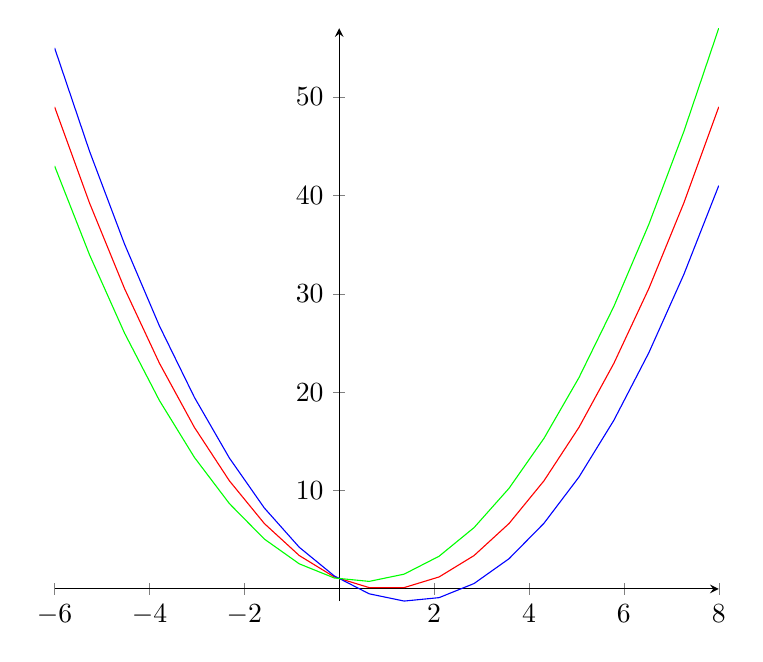
\begin{tikzpicture}
    \begin{axis}[
      scale only axis,
      axis lines=middle,
      ]
      \addplot[
      domain=-6:8,
      samples=20,
      color=red
      ]{x^2 - 2 * 1 * x + 1};
      \addplot[
      domain=-6:8,
      samples=20,
      color=blue
      ]{x^2 - 2 * 1.5 * x + 1};
      \addplot[
      domain=-6:8,
      samples=20,
      color=green
      ]{x^2 - 2 * 0.5 * x + 1};
    \end{axis}
  \end{tikzpicture} \\
  a = {\color{red}1},\; {\color{blue}1.5},\; {\color{green}0.5}
  \end{gather*}
  \item [c]
  \begin{gather*}
    f_a'(4) = 2 \cdot 4 - 2a = 1 \gap\Rightarrow a = 3.5
  \end{gather*}
  \item [d]
  \begin{gather*}
    x_{1/2} = a \pm \sqrt{a^2 - 1} \\
    a^2 - 1 < 0 \gap fuer \; a < 1 \gap \Rightarrow \text{ keine Nullstelle} \\
    a^2 - 1 = 0 \gap fuer \; a = 1 \gap \Rightarrow \text{ 1 Nullstelle} \\
    a^2 - 1 > 0 \gap fuer \; a > 1 \gap \Rightarrow \text{ 2 Nullstellen}
  \end{gather*}
\end{exercise}
\newpage
\subsection{Ortslinie}
Der Graph, auf dem alle Tiefpunkte zu unterschiedlichen $a$ liegen, heißt Ortslinie der Tiefpunkte: \\
\begin{gather*}
  T(a|-a^2 + 1) \\
  x = a \\
  y = -a^2 + 1 \\
  \text{setze $a$ aus $x$-Koordinate in $y$ ein} \\
  f(x) = y = -x^2 + 1 \\
  \text{Funktionsgleichung der Ortskurve der Tiefpunkte}
\end{gather*}
\begin{gather*}
  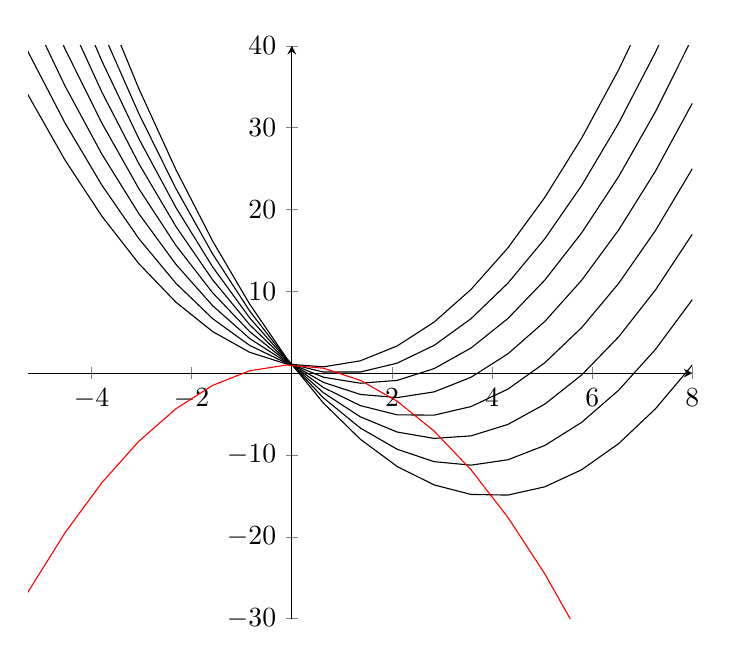
\begin{tikzpicture}
    \begin{axis}[
      scale only axis,
      axis lines=middle,
      ymin=-30,
      ymax=40,
      ]
      \addplot[
      domain=-6:8,
      samples=20
      ]{x^2 - 2 * 0.5 * x + 1};
      \addplot[
      domain=-6:8,
      samples=20
      ]{x^2 - 2 * 1 * x + 1};
      \addplot[
      domain=-6:8,
      samples=20
      ]{x^2 - 2 * 1.5 * x + 1};
      \addplot[
      domain=-6:8,
      samples=20
      ]{x^2 - 2 * 2 * x + 1};
      \addplot[
      domain=-6:8,
      samples=20
      ]{x^2 - 2 * 2.5 * x + 1};
      \addplot[
      domain=-6:8,
      samples=20
      ]{x^2 - 2 * 3 * x + 1};
      \addplot[
      domain=-6:8,
      samples=20
      ]{x^2 - 2 * 3.5 * x + 1};
      \addplot[
      domain=-6:8,
      samples=20
      ]{x^2 - 2 * 4 * x + 1};
      \addplot[
      domain=-6:8,
      samples=20,
      color=red
      ]{-x^2 + 1};
    \end{axis}
  \end{tikzpicture}
\end{gather*}
\newpage
\begin{exercise}{AB/5}
  \item [a]
  \begin{gather*}
    f_a(x) = \frac{1}{2}x^4 - ax^2 \\
    a > 0 \\
    \textbf{Symmetrie} \\
    f_a(-x) = \frac{1}{2}x^4 - ax^2 = f_a(x) \\
    \Rightarrow \text{Achsensymmetrie} \\
    -f_a(x) = -\frac{1}{2}x^4 + ax^2 \neq f_a(-x) \\
    \Rightarrow \text{keine Punktsymmetrie erkennbar} \\
    \textbf{Nullstellen} \\
    \frac{1}{2}x^4 - ax^2 = 0 \equ :x^2 \\
    \frac{1}{2}x^2 - a = 0 \\
    L = \{0; \pm\sqrt{2a}\} \\
    \textbf{Extrema} \\
    f_a'(x) = 2x^3 - 2ax = 0 \equ :x \\
    2x^2 - 2a = 0 \\
    x = \pm\sqrt{a} \\
    f_a''(x) = 6x^2 - 2a \\
    f_a''(\pm\sqrt{a}) = 4a > 0 \Rightarrow TP \\
    f_a''(0) = -2a < 0 \Rightarrow HP \\
    \textbf{Wendepunkte} \\
    f_a''(x) = 0 \gap L = \{\pm\sqrt{\frac{a}{3}}\} \\
    f_a'''(x) = 12x \\
    f_a'''(\sqrt{\frac{a}{3}}) = 12\sqrt{\frac{a}{3}} > 0 \Rightarrow RLWP \\
    f_a'''(-\sqrt{\frac{a}{3}}) = -12\sqrt{\frac{a}{3}} < 0 \Rightarrow LRWP
  \end{gather*}
  \item [b]
  \begin{gather*}
    T(\pm\sqrt{a}|-\frac{1}{2}a^2) \\
    f_T(x) = -\frac{1}{2}x^4 \\\\
    W(\pm\sqrt{\frac{a}{3}}|-\frac{5a^2}{18}) \\
    f_W(x) = -\frac{5}{2}x^4
  \end{gather*}
  \begin{gather*}
    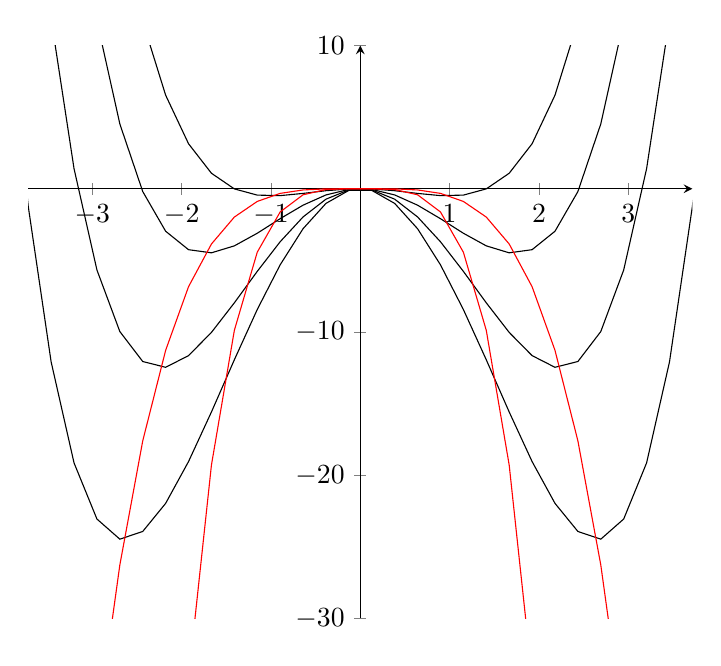
\begin{tikzpicture}
      \begin{axis}[
        scale only axis,
        axis lines=middle,
        ymin=-30,
        ymax=10
        ]
        \addplot[
        samples=40
        ]{1/2 * x^4 - 1 * x^2};
        \addplot[
        samples=40
        ]{1/2 * x^4 - 3 * x^2};
        \addplot[
        samples=40
        ]{1/2 * x^4 - 5 * x^2};
        \addplot[
        samples=40
        ]{1/2 * x^4 - 7 * x^2};
        \addplot[
        samples=40,
        color=red
        ]{-1/2 * x^4};
        \addplot[
        samples=40,
        color=red
        ]{-5/2 * x^4};
      \end{axis}
    \end{tikzpicture}
  \end{gather*}
\end{exercise}
\begin{exercise}{AB/4}
  \item [a]
  \begin{gather*}
    f_a(x) = \frac{1}{4}(x^4 - ax^2) \gap\gap\gap WP(1|f_a(1)) \\
    f_a(-x) = \frac{1}{4}(x^4 - ax^2) = f_a(x) \\
    \Rightarrow \text{Achsensymmetrie} \Rightarrow \text{zweiter Wendepunkt bei } x = -1 \\
    f_a''(\pm1) = 3 \cdot 1^2 - \frac{1}{2}a = 0 \gap\Rightarrow a = 6 \\
    f_6(\pm1) = \frac{1}{4}(1^4 - 6 \cdot 1^2) = -\frac{5}{4}
  \end{gather*}
  \item [b]
  \begin{gather*}
    f_a''(x) = 3x^2 - \frac{1}{2}a = 0 \gap L=\{\pm\sqrt{\frac{a}{6}}\} \\
    t_1(x) = -\frac{a}{3}\sqrt{\frac{a}{6}}x + \frac{a^2}{48} \\
    t_2(x) = \frac{a}{3}\sqrt{\frac{a}{6}}x + \frac{a^2}{48}
  \end{gather*}
\end{exercise}
\section{Wiederholung}
\begin{exercise}{115/9}
  \begin{gather*}
    O(a, h) = a^2 + 4ah \\
    V(a, h) = a^2 \cdot h = 40dm^3 \gap\Rightarrow h = \frac{40dm^3}{a^2} \\
    O(a) = a^2 + 160dm^3 \cdot a^{-1} \\
    O'(a) = 2a - 160dcm^3 \cdot a^{-2} \\
    a = \sqrt[3]{80dm^3} \approx 4.309dm \\
    h = \frac{40dm^3}{\sqrt[3]{80dm^3}^2} = \sqrt[3]{10} \approx 2.154dm
  \end{gather*}
\end{exercise}
\begin{exercise}{119/8}
  \begin{gather*}
    h(0) = 400m \\
    h(370) = 0
  \end{gather*}
  \item [a]
  $h'$ beschreibt das Gefälle des Flusses und gibt den Höhenverlust des Wassers pro Kilometer an
  \item [b]
  ein Stausee hat einen waagerechten Abschnitt des Graphen zur Folge, ein Wasserfall eine Sprungstelle
  \item [c]
  $h'$ ist nicht positiv, da das Wasser ausschließlich nach unten fließt; die Einheit ist $\frac{m}{km}$
\end{exercise}
\section{Sinus- und Kosinusfunktion}
\begin{gather*}
  f(\alpha) = sin(\alpha) \\
  f(x) = sin(x) \\\\
  \frac{\alpha}{360^\circ} = \frac{x}{U} \gap\gap\gap U = 2\pi r \\\\
  x = \frac{\alpha \cdot 2\pi}{360^\circ} \gap\gap\gap \alpha = \frac{x \cdot 360^\circ}{2\pi} \\\\
  \text{wichtige x-Koordinaten} \\
  x = 3.14... = \pi \gap\gap\gap x = 6.28... = 2\pi \\
  x = 1.57... = \frac{\pi}{2} \gap\gap\gap x = 4.71... = \frac{3\pi}{2} \\\\
  sin(x + \frac{\pi}{2}) = cos(x) \gap\gap\gap sin(x) = cos(x - \frac{\pi}{2}) \\\\
\end{gather*}
\subsection{Vielfachheit der Lösungen von (geniometrischen) Gleichungen}
\begin{gather*}
  sin(x) = 0.7 \\
  x = asin(0.7) \approx 0.775 \\
  x_n \approx 0.775 + n \cdot 2\pi \\
  x_m \approx \pi - 0.775 + m \cdot 2\pi \\
  n, m \in \mathbb{Z} \\\\
  cos(x) = 0.3 \\
  x = acos(0.3) \approx 1.266 \\
  x_n \approx 1.266 + n \cdot 2\pi \\
  x_m \approx -1.266 + n \cdot 2\pi \\
  n, m \in \mathbb{Z}
\end{gather*}
\begin{exercise}{128/6}
  \item [a]
  \begin{gather*}
    sin(x) = 0.9396 \\
    x = asin(0.9396) \approx 1.221 \\
    x_n \approx 1.221 + n \cdot 2\pi \\
    x_m \approx \pi - 1.221 + m \cdot 2\pi
  \end{gather*}
  \item [b]
  \begin{gather*}
    sin(x) = 0.5519 \\
    x = asin(0.5519) \approx 0.585 \\
    x_n \approx 0.585 + n \cdot 2\pi \\
    x_m \approx \pi - 0.585 + m \cdot 2\pi
  \end{gather*}
  \item [c]
  \begin{gather*}
    cos(x) = 0.6294 \\
    x = asin(0.6294) \approx 0.890 \\
    x_n \approx 0.890 + n \cdot 2\pi \\
    x_m \approx -0.890 + m \cdot 2\pi
  \end{gather*}
  \item [d]
  \begin{gather*}
    cos(x) = -0.8870 \\
    x = asin(-0.8870) \approx 2.662 \\
    x_n \approx 2.662 + n \cdot 2\pi \\
    x_m \approx -2.662 + m \cdot 2\pi
  \end{gather*}
\end{exercise}
\begin{exercise}{128/7}
  \item [a]
  \begin{gather*}
    sin(x) = 0.63 \\
    x = asin(0.63) \approx 0.682 \\
    x_n \approx 0.682 + n \cdot 2\pi \\
    x_m \approx \pi - 0.682 + m \cdot 2\pi
  \end{gather*}
  \item [b]
  \begin{gather*}
    cos(x) = -0.55 \\
    x = asin(-0.55) \approx 2.153 \\
    x_n \approx 2.153 + n \cdot 2\pi \\
    x_m \approx -2.153 + m \cdot 2\pi
  \end{gather*}
  \item [c]
  \begin{gather*}
    sin(x) = -\frac{1}{2} \\
    x = asin(-\frac{1}{2}) \approx -0.524 \\
    x_n \approx -0.524 + n \cdot 2\pi \\
    x_m \approx \pi + 0.524 + m \cdot 2\pi
  \end{gather*}
  \item [d]
  \begin{gather*}
    cos(x) = -\frac{1}{2}\sqrt{2} \\
    x = asin(-\frac{1}{2}\sqrt{2}) \approx 2.356 \\
    x_n \approx 2.356 + n \cdot 2\pi \\
    x_m \approx -2.356 + m \cdot 2\pi
  \end{gather*}
\end{exercise}
\subsection{Die allgemeine Sinusfunktion}
$$f(x) = y = a \cdot sin(b(x - c)) + d$$
\begin{itemize}
  \item [$a$] Streckung entlang der y-Achse (Amplitude)
  \item [$b$] Streckung entlang der x-Achse (Perioden pro $2\pi$, Periodenlänge $p = \frac{2\pi}{b}$)
  \item [$c$] Verschiebung in x-Richtung (für $c > 0$ nach rechts)
  \item [$d$] Verschiebung in y-Richtung
\end{itemize}
\newpage
\subsection{AB Die Funktionen $f: x \mapsto a \cdot sin(b(x - c))$ und ihre Graphen}
\begin{exercise}{AB/3}
  \item [a]
  \begin{gather*}
    f(x) = 3 \cdot sin(\frac{1}{2}(x - \pi)) \\
    p = 4\pi \\
    3 \cdot sin(\frac{1}{2}(x - \pi)) \\
    x_H = 2\pi + n \cdot p \\
    x_T = n \cdot p \\
    x_W = \pi + \frac{n}{2} \cdot p
  \end{gather*}
  \item [b]
  \begin{gather*}
    f(x) = 2 \cdot sin(\frac{2}{3}x) \\
    p = 3\pi \\
    x_H = \frac{3}{4}\pi + n \cdot p \\
    x_T = 2\frac{1}{4}\pi + n \cdot p \\
    x_W = \frac{n}{2} \cdot p
  \end{gather*}
  \item [c]
  \begin{gather*}
    f(x) = 4 \cdot sin(x - \frac{\pi}{6}) \\
    p = 2\pi \\
    x_H = \frac{2}{3}\pi + n \cdot p \\
    x_T = \frac{5}{3}\pi + n \cdot p \\
    x_W = \frac{\pi}{6} + \frac{p}{2}
  \end{gather*}
\end{exercise}
\newpage
\begin{exercise}{AB/5}
  $$f(x) = a \cdot sin(b \cdot x + e)$$
  \item [a] $$f(x) = 20 \cdot sin(\frac{\pi}{20} \cdot x - \frac{\pi}{2})$$
  \item [b] $$f(x) = 6 \cdot sin(\frac{\pi}{12} \cdot x + \frac{\pi}{4})$$
  \item [c] $$f(x) = 4 \cdot sin(\frac{\pi}{4} \cdot x - \frac{\pi}{2})$$
\end{exercise}
\begin{exercise}{AB/6}
  $$f(t) = a \cdot sin(b(t - c)) \gap\gap\gap -2 \leq t \leq 13$$
  \item [a]
  Die Sonne bewegt sich aus Sicht der Aufnahmen periodisch auf und ab. Ihr Höhenverlauf lässt sich daher über eine Sinuskurve modellieren.
  \item [b]
  $$f(x) = a \cdot sin(\frac{\pi}{12} \cdot (x - 6))$$
\end{exercise}
\subsection{Ableitung der Sinusfunktion}
\begin{gather*}
  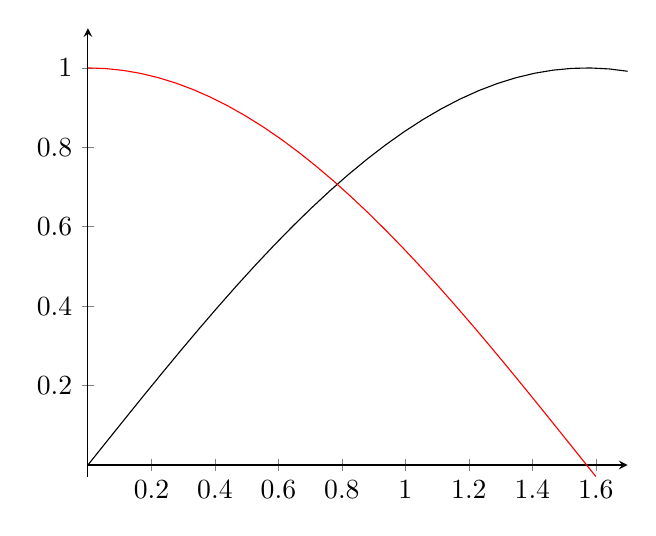
\begin{tikzpicture}
    \begin{axis}[
      axis lines=middle,
      ymax=1.1
      ]
      \addplot[
      domain=0:1.7,
      samples=30
      ]{sin(deg(x))};
      \addplot[
      domain=0:1.6,
      samples=30,
      color=red
      ]{cos(deg(x))};
    \end{axis}
  \end{tikzpicture} \\
  sin(x),\; {\color{red}cos(x)}
\end{gather*}
\subsubsection{Annäherung mit Taylorreihe}
\begin{gather*}
  f(x) = f(a) + \frac{f'(a)}{1!}(x - a)^1 + \frac{f''(a)}{2!}(x - a)^2 + \frac{f'''(a)}{3!}(x - a)^3 + ... \\
  a = x_0 = 0 \\
  f(x_0) = f(0) + \frac{f'(0)}{1!}x^1 + \frac{f''(0)}{2!}x^2 + \frac{f'''(0)}{3!}x^3 + ... \\
  sin(x) = 0 + x^1 - \frac{x^3}{3!} + \frac{x^5}{5!} - \frac{x^7}{7!} + ...\\
  (sin(x))' = 1 - \frac{x^2}{2!} + \frac{x^4}{4!} - \frac{x^6}{6!} = ... = cos(x)
\end{gather*}
\begin{gather*}
  f(x) = sin(x) \\
  f'(x) = cos(x) \\
  f''(x) = -sin(x) \\
  f'''(x) = -cos(x) \\
  f''''(x) = sin(x) \\
  ...
\end{gather*}
\begin{exercise}{130/1}
  \item[a]
  \begin{gather*}
    f(x) = 12 \cdot sin(x) \\
    f'(x) = 12 \cdot cos(x) \\
  \end{gather*}
  \item[b]
  \begin{gather*}
    f(x) = -2 \cdot cos(x) \\
    f'(x) = -2 \cdot (-sin(x)) \\
  \end{gather*}
  \item[c]
  \begin{gather*}
    f(x) = \sqrt{5} \cdot cos(x) \\
    f'(x) = \sqrt{5} \cdot (-sin(x)) \\
  \end{gather*}
  \item[d]
  \begin{gather*}
    f(x) = \frac{1}{\pi} \cdot sin(x) \\
    f'(x) = \frac{1}{\pi} \cdot cos(x) \\
  \end{gather*}
  \item[e]
  \begin{gather*}
    f(x) = 5x^3 - sin(x) \\
    f'(x) = 15x^2 - cos(x) \\
  \end{gather*}
  \item[f]
  \begin{gather*}
    f(x) = 2 \cdot cos(x) - sin(x) \\
    f'(x) = 2 \cdot (-sin(x)) - cos(x) \\
  \end{gather*}
\end{exercise}
\begin{exercise}{130/3}
  \item [b]
  \begin{gather*}
    f(x) = 3 \cdot sin(x) \\
    P(\frac{5\pi}{3}|?) \\
    y = f(\frac{5\pi}{3}) \approx -2.598 \\
    f'(x) = 3 \cdot cos(x) \\
    m_t = f'(\frac{5\pi}{3}) = 1.5 \\
    b_t = -2.598 - 1.5 \cdot \frac{5\pi}{3} \approx -10.452 \\
    t(x) = 1.5x - 10.452
  \end{gather*}
\end{exercise}
\newpage
\begin{exercise}{130/4}
  \item [c]
  \begin{gather*}
    f(x) = 2 \cdot sin(x) - cos(x); \gap x \in \left[0; 2\pi\right] \\
    f'(x) = 2 \cdot cos(x) + sin(x) \\\\
    f'(x) = 0 = 2 \cdot cos(x) + sin(x) \\
    2 = -\frac{sin(x)}{cos(x)} = -tan(x) \gap\Rightarrow\gap x = atan(-2) \\
    L = \{atan(-2) + n\pi\} \gap n \in \{1; 2\} \\\\
    f''(x) = cos(x) - 2 \cdot sin(x) \\
    f''(atan(-2) + \pi) \approx -2.23 < 0 \\
    HP(atan(-2) + \pi|f(atan(-2) + \pi)) = HP(2.034|2.236) \\
    f''(atan(-2) + 2\pi) \approx 2.23 > 0 \\
    TP(atan(-2) + 2\pi|f(atan(-2) + 2\pi)) = TP(5.176|-2.236)
  \end{gather*}
  \item [d]
  \begin{gather*}
    f(x) = 4 \cdot cos(x) + 2x; \gap x \in \left[0; 2\pi\right] \\
    f'(x) = -4 \cdot sin(x) + 2 \\\\
    f'(x) = 0 = -4 \cdot sin(x) + 2 \\
    0.5 = sin(x) \gap\Rightarrow\gap x = asin(0.5) \\
    L = \{asin(0.5); \pi - asin(0.5)\} \\\\
    f''(x) = -4 \cdot cos(x) \\
    f''(asin(0.5)) \approx -3.46 < 0 \\
    HP(asin(0.5)|f(asin(0.5))) = HP(0.524|4.51) \\
    f''(\pi - asin(0.5)) \approx 3.46 > 0 \\
    TP(\pi - asin(0.5)|f(\pi - asin(0.5))) = TP(2.618|1.772)
  \end{gather*}
\end{exercise}
\section{Neue Funktionen aus alten Funktionen}
\begin{gather*}
  \text{gegeben sind} \\
  f(x) = sin(x) \\
  g(x) = \sqrt{x} \\
  h(x) = x^2 + 5 \\\\
  \text{Produkt} \\
  i(x) = f(x) \cdot g(x) = sin(x) \cdot \sqrt{x} \\
  j(x) = h(x) \cdot f(x) = (x^2 + 5) \cdot sin(x) \\\\
  \text{Quotient} \\
  k(x) = \frac{g(x)}{f(x)} = \frac{\sqrt{x}}{sin(x)} \\
  l(x) = \frac{h(x)}{g(x)} = \frac{x^2 + 5}{\sqrt{x}} \\\\
  \text{Verkettung} \\
  m(x) = f(g(x)) = sin(\sqrt{x}) \\
  n(x) = g(f(x)) = \sqrt{sin(x)} \\
  o(x) = f(g(h(x))) = sin(\sqrt{x^2 + 5})
\end{gather*}
\subsection{Ableitungsregeln}
\subsubsection{Produktregel}
\begin{gather*}
  k(x) = f(x) \cdot g(x) \\
  k'(x) = \lim\limits_{h \to 0} \frac{f(x + h) \cdot g(x + h) - f(x) \cdot g(x)}{h} \\
  \;= \lim\limits_{h \to 0} \frac{f(x + h) \cdot g(x + h) {\color{red}- f(x \cdot g(x + h) + f(x) \cdot g(x + h)} - f(x) \cdot g(x)}{h} \\
  \;= \lim\limits_{h \to 0} \frac{{\color{blue}[f(x + h) - f(x)]} \cdot g(x + h) + f(x) \cdot {\color{violet}[g(x + h) - g(x)]}}{h} \\
  \;= \boldsymbol{{\color{blue}f'(x)} \cdot g(x) + f(x) \cdot {\color{violet}g'(x)}}
\end{gather*}
\subsubsection{Kettenregel}
\begin{gather*}
  k(x) = f(g(x)) \\
  k'(x) = \lim\limits_{h \to 0} \frac{f(g(x + h)) - f(g(x))}{h} \\
  \;= \lim\limits_{h \to 0} \frac{f(g(x + h)) - f(g(x))}{{\color{red}g(x + h) - g(x)}} \cdot \frac{{\color{red}g(x + h) - g(x)}}{h} \\
  \;= \lim\limits_{h \to 0} \frac{f(z + i) - f(z)}{i} \cdot g'(x) \\
  \;= f'(z) \cdot g'(x) \\
  \;= \boldsymbol{f'(g(x)) \cdot g'(x)} \\\\
  g(x) = z \gap\gap g(x + h) = z + i
\end{gather*}
\begin{gather*}
  \textbf{Beispiele} \\
  k(x) = (x^2 + 2x - 7) \cdot sin(x) \\
  k'(x) = (2x + 2) \cdot sin(x) + (x^2 + 2x - 7) \cdot cos(x) \\\\
  k(x) = sin(x^3 - 5x) \\
  k'(x) = cos(x^3 - 5x) \cdot (3x^2 - 5)
\end{gather*}
\begin{exercise}{135/1}
  \item [a]
  \begin{gather*}
    f(x) = (x + 2)^4 \\
    f'(x) = 4(x + 2)^3
  \end{gather*}
  \item [b]
  \begin{gather*}
    f(x) = (8x + 2)^3 \\
    f'(x) = 3(8x + 2)^2 \cdot 8 = 24(8x + 2)^2
  \end{gather*}
  \item [c]
  \begin{gather*}
    f(x) = (\frac{1}{2} - 5x)^3 \\
    f'(x) = 3(\frac{1}{2} - 5x)^2 \cdot (-5) = -15(\frac{1}{2} - 5x)^2
  \end{gather*}
  \item [d]
  \begin{gather*}
    f(x) = \frac{1}{4}(x^2 - 5)^2 \\
    f'(x) = \frac{1}{2}(x^2 - 5) \cdot 2x = x^3 - 5x
  \end{gather*}
\end{exercise}
\begin{exercise}{135/2}
  \item [a]
  \begin{gather*}
    f(x) = \frac{1}{(x - 1)^2} \\
    f'(x) = -2(x - 1)^{-3}
  \end{gather*}
  \item [b]
  \begin{gather*}
    f(x) = \frac{1}{(3x - 1)^2} \\
    f'(x) = -2(3x - 1)^{-3} \cdot 3 = -6(3x - 1)^{-3}
  \end{gather*}
  \item [e]
  \begin{gather*}
    f(x) = sin(2x) \\
    f'(x) = cos(2x) \cdot 2 = 2cos(2x)
  \end{gather*}
  \item [f]
  \begin{gather*}
    f(x) = sin(2x + \pi) \\
    f'(x) = cos(2x + \pi) \cdot 2 = 2cos(2x + \pi) = -2cos(2x)
  \end{gather*}
\end{exercise}
\begin{exercise}{138/1}
  \item [g]
  \begin{gather*}
    f(x) = \frac{2}{x} \cdot cos(x) \\
    f'(x) = -2x^{-2} \cdot cos(x) - \frac{2}{x} \cdot sin(x)
  \end{gather*}
  \item [h]
  \begin{gather*}
    f(x) = sin(x) \cdot cos(x) \\
    f'(x) = (cos(x))^2 - (sin(x))^2 = cos(2x)
  \end{gather*}
  \item [i]
  \begin{gather*}
    f(x) = x^2 \cdot sin(x) \\
    f'(x) = 2x \cdot sin(x) + x^2 \cdot cos(x)
  \end{gather*}
  \item [j]
  \begin{gather*}
    f(x) = \frac{1}{\sqrt{x}} \cdot cos(x) \\
    f'(x) = -\frac{cos(x)}{2\sqrt{x^3}} - \frac{sin(x)}{\sqrt{x}}
  \end{gather*}
  \item [k]
  \begin{gather*}
    f(x) = \frac{\pi}{4} \cdot sin(x) \cdot (2 - x) \\
    f'(x) = \frac{\pi}{4} \cdot cos(x) \cdot (2 - x) - \frac{\pi}{4} \cdot sin(x)
  \end{gather*}
  \item [l]
  \begin{gather*}
    f(x) = \sqrt{3} \cdot \sqrt{x} \\
    f'(x) = \frac{\sqrt{3}}{2\sqrt{x}}
  \end{gather*}
\end{exercise}
\begin{exercise}{135/4}
  \item [a]
  \begin{gather*}
    f(x) = 0.25 \cdot sin(2x + \pi) \\
    f'(x) = 0.25 \cdot cos(2x + \pi) \cdot 2 = -0.5 \cdot cos(2x)
  \end{gather*}
  \item [b]
  \begin{gather*}
    f(x) = \frac{2}{3} \cdot sin(\pi - 3x) \\
    f'(x) = \frac{2}{3} \cdot cos(\pi - 3x) \cdot (-3) = 2 \cdot cos(3x)
  \end{gather*}
  \item [c]
  \begin{gather*}
    f(x) = -cos(x^2 + 1) \\
    f'(x) = sin(x^2 + 1) \cdot 2x
  \end{gather*}
  \item [d]
  \begin{gather*}
    f(x) = \frac{1}{3} \cdot (cos(x))^2 \\
    f'(x) = \frac{1}{3} \cdot 2 \cdot cos(x) \cdot (-sin(x)) = -\frac{2}{3} \cdot cos(x) \cdot sin(x)
  \end{gather*}
  \item [e]
  \begin{gather*}
    f(x) = \sqrt{3x} \\
    f'(x) = \frac{1}{2} \cdot \frac{1}{\sqrt{3x}} \cdot 3 = \frac{3}{2\sqrt{3x}}
  \end{gather*}
  \item [f]
  \begin{gather*}
    f(x) = \sqrt{3 + x} \\
    f'(x) = \frac{1}{2} \cdot \frac{1}{\sqrt{3 + x}} \cdot 1 = \frac{1}{2\sqrt{3 + x}}
  \end{gather*}
  \item [g]
  \begin{gather*}
    f(x) = \sqrt{7x - 5} \\
    f'(x) = \frac{1}{2} \cdot \frac{1}{\sqrt{7x - 5}} \cdot 7 = \frac{7}{2 \cdot \sqrt{7x - 5}}
  \end{gather*}
  \item [h]
  \begin{gather*}
    f(x) = \sqrt{7x^2 - 5} \\
    f'(x) = \frac{1}{2} \cdot \frac{1}{\sqrt{7x^2 - 5}} \cdot 14x = \frac{7x}{\sqrt{7x^2 - 5}}
  \end{gather*}
  \item [i]
  \begin{gather*}
    f(x) = \frac{1}{sin(x)} \\
    f'(x) = -\frac{1}{(sin(x))^2} \cdot cos(x) = -\frac{cos(x)}{(sin(x))^2}
  \end{gather*}
\end{exercise}
\subsubsection{Ableitungen mit mehr als zwei Funktionen}
\begin{gather*}
  l = g \cdot [h \cdot k] \\
  l' = g' \cdot h \cdot k + g \cdot [h' \cdot k + h \cdot k'] \\
  \;= g' \cdot h \cdot k + g \cdot h' \cdot k + g \cdot h \cdot k' \\\\
  l = g(h(k)) \\
  l' = g'(h(k)) \cdot h'(k) \cdot k' \\\\
  l = g \cdot h(k) \\
  l' = g' \cdot h(k) + g \cdot h'(k) \cdot k' \\\\
  l = g(h \cdot k) \\
  l' = g'(h \cdot k) \cdot [h' \cdot k + h \cdot k']
\end{gather*}
\subsubsection{Quotientenregel}
\begin{gather*}
  l = \frac{g}{h} = g \cdot h^{-1} \\
  l' = g' \cdot h^{-1} + g \cdot [-h^{-2} \cdot h'] \\
  \;= g' \cdot h^{-1} - g \cdot h^{-2} \cdot h' \\
  \;= \frac{g'}{h} - \frac{g \cdot h'}{h^2} = \frac{g' \cdot h}{h \cdot h} - \frac{g \cdot h'}{h^2} \\
  \;= \boldsymbol{\frac{g' \cdot h - g \cdot h'}{h^2}}
\end{gather*}
\begin{exercise}{138/2}
  \item [e]
  \begin{gather*}
    f(x) = (5 - 4x)^3 \cdot x^{-2} \\
    f'(x) = 3(5 - 4x)^2 \cdot (-4) \cdot x^{-2} + (5 - 4x)^3 \cdot (-2x^{-3}) \\
    \;= -\frac{2 \cdot (5 - 4x)^2 \cdot (2x + 5)}{x^3}
  \end{gather*}
  \item [f]
  \begin{gather*}
    f(x) = 3x \cdot cos(2x) \\
    f'(x) = 3 \cdot cos(2x) + 3x \cdot (-sin(2x)) \cdot 2 \\
    \;= 3 \cdot (cos(2x) - 2x \cdot sin(2x))
  \end{gather*}
  \item [g]
  \begin{gather*}
    f(x) = 3x \cdot (sin(x))^2 \\
    f'(x) = 3 \cdot (sin(x))^2 + 3x \cdot 2 \cdot sin(x) \cdot cos(x) \\
    \;= 3 \cdot sin(x) \cdot (sin(x) + 2x \cdot cos(x))
  \end{gather*}
  \item [h]
  \begin{gather*}
    f(x) = (2x - 1)^2 \cdot \sqrt{x} \\
    f'(x) = 2(2x - 1) \cdot 2 \cdot \sqrt{x} + (2x - 1)^2 \cdot \frac{1}{2\sqrt{x}} \\
    \;= \frac{(2x - 1) \cdot (10x - 1)}{2\sqrt{x}}
  \end{gather*}
  \item [i]
  \begin{gather*}
    f(x) = 0.5x^2 \cdot \sqrt{4 - x} \\
    f'(x) = x \cdot \sqrt{4 - x} + 0.5x^2 \cdot \frac{1}{2\sqrt{4 - x}} \cdot (-1) \\
    \;= \frac{(4 - 1.25x) \cdot x}{\sqrt{4 - x}}
  \end{gather*}
\end{exercise}
\begin{exercise}{140/2}
  \item [a]
  \begin{gather*}
    f(x) = \frac{1 - x^2}{3x + 5} \\
    f'(x) = \frac{-2x \cdot (3x + 5) - (1 - x^2) \cdot 3}{(3x + 5)^2} \\
    \;= -\frac{(3x + 1) \cdot (x + 3)}{(3x + 5)^2}
  \end{gather*}
  \item [b]
  \begin{gather*}
    g(x) = \frac{\sqrt{x}}{x + 2} \\
    g'(x) = \frac{\frac{1}{2\sqrt{x}} \cdot (x + 2) - \sqrt{x} \cdot 1}{(x + 2)^2} \\
    \;= \frac{2 - x}{2\sqrt{x} \cdot (x + 2)^2}
  \end{gather*}
  \item [c]
  \begin{gather*}
    h(x) = \frac{3 \cdot sin(x)}{6x - 1} \\
    h'(x) = \frac{3 \cdot cos(x) \cdot (6x - 1) - 3 \cdot sin(x) \cdot 6}{(6x - 1)^2}
  \end{gather*}
  \item [d]
  \begin{gather*}
    k(x) = \frac{sin(x)}{cos(x)} \\
    k'(x) = \frac{cos(x) \cdot cos(x) - sin(x) \cdot (-sin(x))}{(cos(x))^2} \\
    \;= 1 + (tan(x))^2
  \end{gather*}
\end{exercise}
\section{Exponentialfunktionen - Ableitung}
\begin{gather*}
  {\color{blue}f(x) = 2^x} \gap\gap {\color{cyan}f'(x)} \gap\gap\gap\gap\gap {\color{red}g(x) = 4^x} \gap\gap {\color{purple}g'(x)}\\
\end{gather*}
\begin{gather*}
  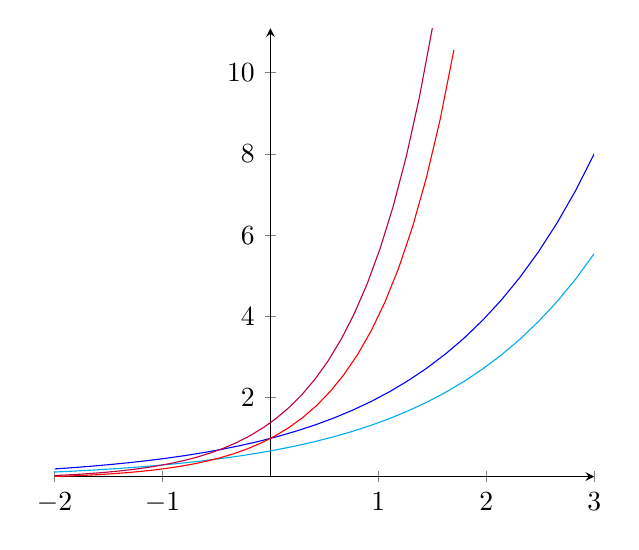
\begin{tikzpicture}
    \begin{axis}[
      axis lines=middle,
      ]
      \addplot[
      domain=-2:3,
      samples=30,
      color=blue
      ]{2^x};
      \addplot[
      domain=-2:3,
      samples=30,
      color=cyan
      ]{2^x * ln(2)};
      \addplot[
      domain=-2:1.7,
      samples=30,
      color=red
      ]{4^x};
      \addplot[
      domain=-2:1.5,
      samples=30,
      color=purple
      ]{4^x * ln(4)};
    \end{axis}
  \end{tikzpicture}
\end{gather*}
Zwischen $2^x$ und $4^x$ liegt eine Exponentialfunktion, deren Ableitungsfunktion genau der Ursprungsfunktion entspricht. Sie wird natürliche Exponentialfunktion genannt.
$$f(x) = e^x$$
$$\text{Eulersche Zahl } e = \lim\limits_{n \to \infty} (1 + \frac{1}{n})^n \approx 2.71828$$
\begin{gather*}
  f(x) = e^x \\
  f'(x) = e^x \\
  f''(x) = e^x \\
  ... \\\\
  e^x \leftrightarrow log_e(x) = ln(x) \\
  \Rightarrow e^{ln(x)} = ln(e^x) = x \\\\
  2^x = 5^{x \cdot \frac{log(2)}{log(5)}} = 5^{x \cdot log_5(2)} \\
  2^x = e^{x \cdot ln(2)} \\
  10^x = e^{x \cdot ln(10)} \\\\
  f(x) = e^{x \cdot ln(2)} = 2^x \\
  f'(x) = e^{x \cdot ln(2)} \cdot ln(2) = 2^x \cdot ln(2) \approx 2^x \cdot 0.7 \\\\
  f(x) = e^{x \cdot ln(4)} = 4^x \\
  f'(x) = e^{x \cdot ln(4)} \cdot ln(4) = 4^x \cdot ln(4) \approx 4^x \cdot 1.4
\end{gather*}
\begin{exercise}{142/3}
  \item [a]
  \begin{gather*}
    f(x) = x \cdot e^x \\
    f'(x) = 1 \cdot e^x + xe^x = e^x \cdot (x + 1)
  \end{gather*}
  \item [b]
  \begin{gather*}
    f(x) = \frac{e^x}{x} \\
    f'(x) = \frac{e^x \cdot x - e^x \cdot 1}{x^2} = \frac{e^x \cdot (x - 1)}{x^2}
  \end{gather*}
  \item [c]
  \begin{gather*}
    f(x) = \frac{x}{e^x} \\
    f'(x) = \frac{1 \cdot e^x - x \cdot e^x}{(e^x)^2} = \frac{1 - x}{e^x}
  \end{gather*}
  \item [d]
  \begin{gather*}
    f(x) = (x + 1) \cdot e^x \\
    f'(x) = 1 \cdot e^x + (x + 1) \cdot e^x = e^x \cdot (x + 2)
  \end{gather*}
  \item [e]
  \begin{gather*}
    f(x) = \frac{x}{e^{-0.5x}} \\
    f(x) = \frac{1 \cdot e^{-0.5x} - x \cdot (-0.5) \cdot e^{-0.5x}}{(e^{-0.5x})^2} = e^{0.5x} \cdot (1 + 0.5x)
  \end{gather*}
  \item [f]
  \begin{gather*}
    f(x) = \frac{e^x + 1}{x} \\
    f'(x) = \frac{e^x \cdot x - (e^x + 1) \cdot 1}{x^2} = \frac{e^x \cdot (x - 1) - 1}{x^2}
  \end{gather*}
  \item [g]
  \begin{gather*}
    f(x) = \frac{e^x}{x - 1} \\
    f'(x) = \frac{e^x \cdot (x - 1) - e^x \cdot 1}{(x - 1)^2} = \frac{e^x \cdot (x - 2)}{(x - 1)^2}
  \end{gather*}
  \item [h]
  \begin{gather*}
    f(x) = \frac{e^{3x}}{x + 2} \\
    f'(x) = \frac{3 \cdot e^{3x} \cdot (x + 2) - e^{3x} \cdot 1}{(x + 2)^2} = \frac{e^{3x} \cdot (3x + 5)}{(x + 2)^2}
  \end{gather*}
  \item [i]
  \begin{gather*}
    f(x) = x^2 + x \cdot e^{0.1x} = x^2 \cdot (1 + \frac{e^{0.1x}}{x}) \\
    f'(x) = 2x \cdot (1 + \frac{e^{0.1x}}{x}) + x^2 \cdot \frac{e^{0.1x} \cdot (0.1x - 1)}{x^2} = e^{0.1x} \cdot (0.1x + 1) + 2x
  \end{gather*}
  \item [j]
  \begin{gather*}
    f(x) = x \cdot e^{-2x + 1} \\
    f'(x) = 1 \cdot e^{-2x + 1} + x \cdot (-2e^{-2x + 1}) = e^{1 - 2x} \cdot (1 - 2x)
  \end{gather*}
  \item [k]
  \begin{gather*}
    f(x) = x^2 \cdot e^{ax} \\
    f'(x) = 2x \cdot e^{ax} + x^2 \cdot a \cdot e^{ax} = x \cdot e^{ax} \cdot (2 + ax)
  \end{gather*}
  \item [l]
  \begin{gather*}
    f(x) = x \cdot e^{2x^2 + 1} \\
    f'(x) = 1 \cdot e^{2x^2 + 1} + x \cdot e^{2x^2 + 1} \cdot 4x = e^{2x^2 + 1} \cdot (4x^2 + 1)
  \end{gather*}
\end{exercise}
\subsection{Basis $\neq e$}
\begin{gather*}
  f(x) = 10^x = (e^z)^x = e^{ln(10) \cdot x} \\
  e^z = 10 \gap\Rightarrow\gap z = ln(10) \\
  \Rightarrow\gap b^x = e^{ln(b) \cdot x} \\\\
  f'(x) = e^{ln(10) \cdot x} \cdot ln(10) \\
  \;= 10^x \cdot ln(10) \\
  \Rightarrow\gap b^x \cdot ln(b)
\end{gather*}
\begin{exercise}{145/8}
  \item [f]
  \begin{gather*}
    e^{2x} + 10 = 6.5 \cdot e^x \equ \text{subst. } e^x = z \\
    z^2 + 10 = 6.5z \equ - 6.5z \\
    z^2 - 6.5z + 10 = 0 \\
    z_{1/2} = \frac{6.5 \pm \sqrt{42.25 - 40}}{2} \\
    z_1 = 4 \gap z_2 = 2.5 \equ \text{resubst.} \\\\
    z_1 = 4 = e^x \equ ln \\
    x_1 = ln(4) \approx 1.386 \\\\
    z_2 = 2.5 = e^x \equ ln \\
    x_2 = ln(2.5) \approx 0.916
  \end{gather*}
  \item [a]
  \begin{gather*}
    e^{2x} - 6 \cdot e^x + 8 = 0 \equ \text{subst. } e^x = z \\
    z^2 - 6z + 8 = 0 \\
    z_{1/2} = \frac{6 \pm \sqrt{36 - 32}}{2} \\
    z_1 = 4 \gap z_2 = 2 \equ \text{resubst.} \\\\
    z_1 = 4 = e^x \equ ln \\
    x_1 = ln(4) \approx 1.386 \\\\
    z_2 = 2 \equ ln \\
    x_2 = ln(2) \approx 0.693
  \end{gather*}
  \item [b]
  \begin{gather*}
    e^x - 2 - \frac{15}{e^x} = 0 \equ \text{subst. } e^x = z \\
    z - 2 - \frac{15}{z} = 0 \equ \cdot z \\
    z^2 - 2z - 15 = 0 \\
    z_{1/2} = \frac{2 \pm \sqrt{4 + 60}}{2} \\
    z_1 = 5 \gap (z_2 = -3) \equ \text{resubst.} \\\\
    z_1 = 5 = e^x \equ ln \\
    x_1 = ln(5) \approx 1.609
  \end{gather*}
  \item [g]
  \begin{gather*}
    (e^{2x} - 6) \cdot (5 - e^{3x}) = 0 \equ \text{subst. } e^x = z \\
    (z^2 - 6) \cdot (5 - z^3) = 0 \\\\
    z^2 - 6 = 0 \equ \sqrt{} \\
    z_1 = \sqrt{6} \approx 2.449 \equ \text{resubst.} \\
    z_1 = \sqrt{6} = e^x \equ ln \\
    x_1 = ln(\sqrt{6}) \approx 0.896 \\\\
    5 - z^3 = 0 \equ \sqrt[3]{} \\
    z_2 = \sqrt[3]{5} \approx 1.710 \equ \text{resubst.} \\
    z_2 = \sqrt[3]{5} = e^x \equ ln \\
    x_2 = ln(\sqrt[3]{5}) \approx 0.536
  \end{gather*}
  \item [h]
  \begin{gather*}
    2 \cdot e^x + 15 = 8 \cdot e^{-x} \equ \text{subst. } e^x = z \\
    2z + 15 = \frac{8}{z} \equ -\frac{8}{z} \\
    2z + 15 - \frac{8}{z} = 0 \equ \cdot z \\
    2z^2 + 15z - 8 = 0 \\
    z_{1/2} = \frac{-15 \pm \sqrt{225 + 64}}{4} \\
    z_1 = 0.5 \gap (z_2 = -8) \equ \text{resubst.} \\\\
    z_1 = 0.5 = e^x \equ ln \\
    x = ln(0.5) \approx -0.693
  \end{gather*}
\end{exercise}
\begin{exercise}{146/9}
  \begin{gather*}
    h(t) = 0.02 \cdot e^{kt}
  \end{gather*}
  \item [a]
  \begin{gather*}
    h(0) = 0.02
  \end{gather*}
  \item [b]
  \begin{gather*}
    h(6) = 0.02 \cdot e^{6k} = 0.4 \\
    e^{6k} = 20 \\
    6k = ln(20) \\
    k = \frac{ln(20)}{6} \approx 0.499
  \end{gather*}
  \item [c]
  \begin{gather*}
    h(9) = 0.02 \cdot e^{0.499 \cdot 9} \approx 1.784
  \end{gather*}
  \item [d]
  \begin{gather*}
    h(t) = 0.02 \cdot e^{0.499t} = 3 \\
    e^{0.499t} = 150 \\
    0.499t = ln(150) \\
    t = \frac{ln(150)}{0.499} \approx 10.041
  \end{gather*}
  \item [e]
  \begin{gather*}
    h(t + 1) - h(t) = 1.5 \\
    0.02 \cdot e^{k \cdot (t + 1)} - 0.02 \cdot e^{k \cdot t} = 1.5 \\
    0.02e^{kt} \cdot (e^k - 1) = 1.5 \\
    e^{kt} \cdot (e^k - 1) = 75 \\
    0.647e^{0.499t} = 75 \\
    e^{0.499t} = 115.92 \\
    0.499t = ln(115.92) \\
    t = \frac{ln(115.92)}{0.499} \approx 9.525
  \end{gather*}
  \item [f]
  \begin{gather*}
    h'(t) = 0.02k \cdot e^{kt} = 1 \\
    0.02 \cdot 0.499 \cdot e^{0.499t} = 1 \\
    e^{0.499t} = 100.2 \\
    0.499t = ln(100.2) \\
    t = \frac{ln(100.2)}{0.499} \approx 9.233
  \end{gather*}
  \item [g]
  \begin{gather*}
    t \geq 9 \\
    k(t) = 3.5 - 8.2 \cdot e^{-0.175t} \\\\
    k(t) = 3.5 - 8.2 \cdot e^{-0.175t} = 3 \\
    e^{-0.175t} \approx 0.061 \\
    -0.175t \approx ln(0.061) \\
    t \approx \frac{ln(0.061)}{-0.175} \approx 15.982 \\\\
    k(t + 1) - k(t) = 0.2 \\
    3.5 - 8.2 \cdot e^{-0.175 \cdot (t + 1)} - 3.5 + 8.2 \cdot e^{-0.175t} = 0.2 \\
    -8.2 \cdot e^{-0.175 \cdot (t + 1)} + 8.2 \cdot e^{-0.175t} = 0.2 \\
    -8.2 \cdot e^{-0.175t} \cdot (e^{-0.175} - 1) = 0.2 \\
    1.316 \cdot e^{-0.175t} \approx 0.2 \\
    e^{-0.175t} \approx 0.152 \\
    -0.175t \approx ln(0.152) \\
    t \approx \frac{ln(0.152)}{-0.175} \approx 10.765
  \end{gather*}
\end{exercise}
\newpage
\section{Wiederholung}
\subsection{Sinusfunktionen und Newton-Verfahren}
\begin{exercise}{130/8}
  \begin{gather*}
    P(x_0|f(x_0)) \gap\gap Q(x_0|g(x_0)) \gap\gap 0 \leq x \leq 2\pi
  \end{gather*}
  \item [a]
  \begin{gather*}
    f(x) = 2 \cdot sin(x) \gap\gap g(x) = x^2 \\
    f'(x) = 2 \cdot cos(x) \gap\gap g'(x) = 2x \\
    h(x) = f'(x) - g'(x) = 2 \cdot cos(x) - 2x = 0 \\
    h'(x) = -2 \cdot sin(x) - 2 \\\\
    x_0 = 0 \\
    x_1 = x_0 - \frac{h(x_0)}{h'(x_0)} = 1 \\
    x_2 = x_1 - \frac{h(x_1)}{h'(x_1)} \approx 0.75036 \\
    x_3 = x_2 - \frac{h(x_2)}{h'(x_2)} \approx 0.73911 \\
    x_4 = x_3 - \frac{h(x_3)}{h'(x_3)} \approx 0.73908 \\
    x_5 = x_4 - \frac{h(x_4)}{h'(x_4)} \approx 0.73909 \\
    x^\ast \approx 0.7391 \\\\
    P(x^\ast|f(x^\ast)) \approx P(0.7391|1.3472) \\
    Q(x^\ast|g(x^\ast)) \approx Q(0.7391|0.5463)
  \end{gather*}
  \item [b]
  \begin{gather*}
    f(x) = sin(x) + 2 \cdot cos(x) \gap\gap g(x) = x^3 \\
    f'(x) = cos(x) - 2 \cdot sin(x) \gap\gap g'(x) = 3x^2 \\
    h(x) = f'(x) - g'(x) = cos(x) - 2 \cdot sin(x) - 3x^2 = 0 \\
    h'(x) = -sin(x) - 2 \cdot cos(x) - 6x \\\\
    x_0 = 0 \\
    x_1 = x_0 - \frac{h(x_0)}{h'(x_0)} = 0.5 \\
    x_2 = x_1 - \frac{h(x_1)}{h'(x_1)} \approx 0.34120 \\
    x_3 = x_2 - \frac{h(x_2)}{h'(x_2)} \approx 0.32336 \\
    x_4 = x_3 - \frac{h(x_3)}{h'(x_3)} \approx 0.32311 \\
    x_5 = x_4 - \frac{h(x_4)}{h'(x_4)} \approx 0.32311 \\
    x^\ast \approx 0.3231 \\\\
    P(x^\ast|f(x^\ast)) \approx P(0.3231|2.2140) \\
    Q(x^\ast|g(x^\ast)) \approx Q(0.3231|0.0337)
  \end{gather*}
\end{exercise}
\subsection{Produktregel}
\begin{exercise}{138/3}
  \item [a]
  \begin{gather*}
    f(x) = (2x - 8) \cdot sin(x) \gap\gap f'(x) = 2 \cdot cos(x) \\
    f(x) = a \cdot b \gap\gap f'(x) = a' \cdot b + a \cdot b' \neq a' \cdot b' \\
    \Rightarrow \gap f'(x) = 2 \cdot sin(x) + (2x - 8) \cdot cos(x)
  \end{gather*}
  \item [b]
  \begin{gather*}
    g(x) = (2x - 3) \cdot (8 - x)^2 \\
    g'(x) = \textbf{2} \cdot (8 - x)^2 + (2x - 3) \cdot \textbf{(16 - 2x)}
  \end{gather*}
\end{exercise}
\subsection{Quotientenregel}
\begin{exercise}{140/11}
  \item [a]
  \begin{gather*}
    f(x) = sin(x) + tan(x) = sin(x) + \frac{sin(x)}{cos(x)} \\
    f'(x) = cos(x) + (cos(x))^{-2}
  \end{gather*}
  \item [b]
  \begin{gather*}
    f(x) = sin(x) \cdot tan(x) = \frac{(sin(x))^2}{cos(x)} \\
    f'(x) = sin(x) + \frac{sin(x)}{(cos(x))^2}
  \end{gather*}
  \item [c]
  \begin{gather*}
    f(x) = \frac{cos(x)}{tan(x)} = \frac{(cos(x))^2}{sin(x)} \\
    f'(x) = -2 \cdot cos(x) - \frac{(cos(x))^3}{(sin(x))^2}
  \end{gather*}
  \item [d]
  \begin{gather*}
    f(x) = \frac{tan(x)}{2} = \frac{sin(x)}{2 \cdot cos(x)} \\
    f'(x) = \frac{1}{2 \cdot (cos(x))^2}
  \end{gather*}
  \item [e]
  \begin{gather*}
    f(x) = tan(2x) = \frac{sin(2x)}{cos(2x)} \\
    f'(x) = \frac{2}{(cos(2x))^2}
  \end{gather*}
  \item [f]
  \begin{gather*}
    f(x) = tan(x^2) = \frac{sin(x^2)}{cos(x^2)} \\
    f'(x) = \frac{2x}{(cos(x^2))^2}
  \end{gather*}
  \item [g]
  \begin{gather*}
    f(x) = (tan(x))^2 = \frac{(sin(x))^2}{(cos(x))^2} \\
    f'(x) = \frac{2 \cdot sin(x)}{(cos(x))^3}
  \end{gather*}
  \item [h]
  \begin{gather*}
    f(x) = \frac{2}{tan(x)} = \frac{2 \cdot cos(x)}{sin(x)} \\
    f'(x) = -\frac{2}{(sin(x))^2}
  \end{gather*}
\end{exercise}
\subsection{Kurvendiskussion}
\begin{exercise}{146/13}
  \begin{gather*}
    f(x) = 80000 \cdot e^{0.002x} \\
    0 \estim 01.10.2002
  \end{gather*}
  \item [a]
  \begin{gather*}
    92 \estim 01.01.2003 \\
    f(92) = 80000 \cdot e^{0.002 \cdot 92} \approx 96161.27 \\
    457 \estim 01.01.2004 \\
    f(457) = 80000 \cdot e^{0.002 \cdot 457} \approx 199542.38 \\
  \end{gather*}
  \item [b]
  \begin{gather*}
    f(x) = 80000 \cdot e^{0.002x} = 1000000 \\
    e^{0.002x} = 12.5 \\
    x = \frac{ln(12.5)}{0.002} \approx 1262.86 \estim 17.03.2006 \\\\
    f(x) = 80000 \cdot e^{0.002x} = 1000000000 \\
    e^{0.002x} = 12500 \\
    x = \frac{ln(12500)}{0.002} \approx 4716.74 \estim 31.08.2015
  \end{gather*}
  \item [c]
  \begin{gather*}
    2 \cdot f(x_1) = f(x_2) \\
    2 \cdot 80000 \cdot e^{0.002x_1} = 80000 \cdot e^{0.002x_2} \\
    2 \cdot e^{0.002x_1} = e^{0.002x_2} \\
    ln(2) + 0.002x_1 = 0.002x_2 \\
    x_2 - x_1 = \frac{ln(2)}{0.002} \approx 346.57
  \end{gather*}
  \item [d]
  \begin{gather*}
    p \cdot f(x_1) = f(x_1 + 365) \\
    p \cdot 80000 \cdot e^{0.002x_1} = 80000 \cdot e^{0.002 \cdot (x_1 + 365)} \\
    p \cdot e^{0.002x_1} = e^{0.002x_1} \cdot e^{0.002 \cdot 365} \\
    p = e^{0.002 \cdot 365} \approx 2.08 = 208\%
  \end{gather*}
  \item [e]
  \begin{gather*}
    365 \estim 01.10.2003 \\
    f(365) - f(364) = 80000 \cdot e^{0.002 \cdot 365} - 80000 \cdot e^{0.002 \cdot 364} \approx 331.68 \\\\
    f'(x) = 80000 \cdot 0.002 \cdot e^{0.002x} = 160 \cdot e^{0.002x} \\
    f(364.5) \approx 331.68
  \end{gather*}
  \item [f]
  \begin{gather*}
    f(x + 1) - f(x) = 400 \\
    80000 \cdot e^{0.002 \cdot (x + 1)} - 80000 \cdot e^{0.002x} = 400 \\
    80000 \cdot e^{0.002x} \cdot (e^{0.002} - 1) = 400 \\
    x = ln(\frac{400}{80000 \cdot (e^{0.002} - 1)}) \cdot \frac{1}{0.002} \approx 457.65 \estim 02.01.2004 \\\\
    f'(x) = 160 \cdot e^{0.002x} = 400 \\
    x = ln(\frac{400}{160}) \cdot \frac{1}{0.002} \approx 458.15 \estim 03.01.2004
  \end{gather*}
\end{exercise}
\newpage
\begin{exercise}{146/10}
  \begin{gather*}
    v(t) = 2.5 \cdot (1 - e^{-0.1t})
  \end{gather*}
  \item [a]
  \begin{gather*}
    v(0) = 0 \\
    v(10) \approx 1.58
  \end{gather*}
  \item [b]
  \begin{gather*}
    \begin{tikzpicture}
      \begin{axis}[
        axis lines=middle
        ]
        \addplot[
        domain=0:20,
        samples=100
        ]{2.5 * (1 - e^(-0.1 * x))};
      \end{axis}
    \end{tikzpicture}
  \end{gather*}
  \item [c]
  \begin{gather*}
    v(t) = 2 \\
    t = -\frac{ln(0.2)}{0.1} \approx 16.09
  \end{gather*}
  \item [d]
  \begin{gather*}
    \lim\limits_{t \to \infty} v(t) = 2.5
  \end{gather*}
  \item [e]
  \begin{gather*}
    v(t) = 2.5 \cdot (1 - e^{-0.1t}) \\
    v(t + 1) = 2.5 \cdot (1 - e^{-0.1 \cdot (t + 1)}) \\\\
    v(t) < v(t + 1) \\
    2.5 \cdot (1 - e^{-0.1t}) < 2.5 \cdot (1 - e^{-0.1 \cdot (t + 1)}) \equ : 2.5 \\
    1 - e^{-0.1t} < 1 - e^{-0.1 \cdot (t + 1)} \equ - 1; \cdot (-1) \\
    e^{-0.1t} > e^{-0.1 \cdot (t + 1)} \equ ln() \\
    -0.1t > -0.1 \cdot (t + 1) \equ \cdot (-10) \\
    t < t + 1
  \end{gather*}
  \item [f]
  \begin{gather*}
    \Delta v = v(t_2) - v(t_1) \\
    \;= v(5) - v(2) \approx 0.98 - 0.45 = 0.53
  \end{gather*}
  \item [g]
  \begin{gather*}
    v'(t) = 0.25 \cdot e^{-0.1t} \\
    v'(2) = 0.20
  \end{gather*}
  \item [h]
  Die Beschleunigung ist bei $t = 0$ am größten, da sie ständig kleiner wird.
\end{exercise}
\section{Lineare Gleichungssysteme (LGS)}
\begin{gather*}
  \text{z. B.} \gap
  \begin{vmatrix}
    3x_1 & + & 2x_2 & - & 3x_3 & = & 5 \\
    -x_1 & - & x_2 & + & 5x_3 & = & 15
  \end{vmatrix}
  \gap \text{2x3 LGS}
\end{gather*}
\subsubsection{LGS in Stufenform}
\begin{gather*}
  \begin{vmatrix}
    -x_2 & + & 4x_1 & + & 3x_3 & = 2 \\
    3x_2 & + & x_1 &&&  = 5 \\
    4x_2 &&&&& = 8
  \end{vmatrix} \\
  \Rightarrow \text{ einfach zu lösen} \\
  \text{\Rmnum{3}} \gap 4x_2 = 8 \rightarrow x_2 = 2 \\
  \text{eingesetzt in \Rmnum{2}} \\
  x_1 + 3 \cdot 2 = 5 \rightarrow x_1 = -1 \\
  \text{eingesetzt in \Rmnum{1}} \\
  4 \cdot (-1) -2 + 3x_3 = 2 \rightarrow x_3 = \frac{8}{3} \\
  L = \{(-1|2|\frac{8}{3})\}
\end{gather*}
\subsection{Gauß-Verfahren}
Das Gauß-Verfahren dient dazu, ein LGS in Stufenform zu überführen und dann zu lösen.
\newpage
\begin{exercise}{256/4}
  \item [a]
  \begin{gather*}
    \begin{vmatrix}
      2x_1 & - & 4x_2 & + & 5x_3 & = & 3 \\
      3x_1 & + & 3x_2 & + & 7x_3 & = & 13 \\
      4x_1 & - & 2x_2 & - & 3x_3 & = & -1
    \end{vmatrix}
  \end{gather*}
  Eliminiere $x_1$ aus 2 der 3 Gleichungen
  \begin{gather*}
    \begin{vmatrix}
      2x_1 & - & 4x_2 & + & 5x_3 & = & 3 \\
      3x_1 & + & 3x_2 & + & 7x_3 & = & 13 \\
      {\color{red}0}x_1 & + & 6x_2 & - & 13x_3 & = & -7
    \end{vmatrix}
    \gap\gap \Rmnum{3} - 2 \cdot \Rmnum{1} \\
    \begin{vmatrix}
      2x_1 & - & 4x_2 & + & 5x_3 & = & 3 \\
      {\color{red}0}x_1 & + & 18x_2 & - & 1x_3 & = & 17 \\
      {\color{red}0}x_1 & + & 6x_2 & - & 13x_3 & = & -7
    \end{vmatrix}
    \gap\gap 2 \cdot \Rmnum{2} - 3 \cdot \Rmnum{1}
  \end{gather*}
  Eliminiere $x_2$ aus 1 der 2 Gleichungen
  \begin{gather*}
    \begin{vmatrix}
      2x_1 & - & 4x_2 & + & 5x_3 & = & 3 \\
      {\color{red}0}x_1 & + & {\color{red}0}x_2 & + & 38x_3 & = & 38 \\
      {\color{red}0}x_1 & + & 6x_2 & - & 13x_3 & = & -7
    \end{vmatrix}
    \gap\gap \Rmnum{2} - 3 \cdot \Rmnum{3}
  \end{gather*}
  Löse LGS in Stufenform
  \begin{gather*}
    \begin{vmatrix}
      2x_1 & - & 4x_2 & + & 5x_3 & = & 3 \\
      &&&& 38x_3 & = & 38 \\
      && 6x_2 & - & 13x_3 & = & -7
    \end{vmatrix} \\
    \text{\Rmnum{2}} \gap 38x_3 = 38 \rightarrow x_3 = 1 \\
    \text{eingesetzt in \Rmnum{3}} \\
    6x_2 - 13 \cdot 1 = -7 \rightarrow x_2 = 1 \\
    \text{eingesetzt in \Rmnum{1}} \\
    2x_1 - 4 \cdot 1 + 5 \cdot 1 = 3 \rightarrow x_1 = 1 \\
    L = \{(1|1|1)\}
  \end{gather*}
\end{exercise}
\newpage
\subsection{Matrix-Schreibweise}
\begin{exercise}{256/4}
  \item [b]
  \begin{gather*}
    \begin{vmatrix}
      -x_1 & + & 7x_2 & - & x_3 & = & 5 \\
      4x_1 & - & x_2 & + & x_3 & = & 1 \\
      5x_1 & - & 3x_2 & + & x_3 & = & -1
    \end{vmatrix} \gap\longrightarrow\gap
    \begin{vmatrix}
      -1 & 7 & -1 & \vdots & 5 \\
      4 & -1 & 1 & \vdots & 1 \\
      5 & -3 & 1 & \vdots & -1
    \end{vmatrix} \\\\
    \begin{vmatrix}
      -1 & 7 & -1 & \vdots & 5 \\
      3 & 6 & 0 & \vdots & 6 \\
      1 & -2 & 0 & \vdots & -2
    \end{vmatrix} \gap\gap \Rmnum{2} + \Rmnum{1}; \gap \Rmnum{3} - \Rmnum{2} \\
    \begin{vmatrix}
      -1 & 7 & -1 & \vdots & 5 \\
      3 & 6 & 0 & \vdots & 6 \\
      0 & 12 & 0 & \vdots & 12
    \end{vmatrix} \gap\gap \Rmnum{2} - 3 \cdot \Rmnum{3} \\\\
    ... \\
    L = \{0|1|2\}
  \end{gather*}
  \item [c]
  \begin{gather*}
    \begin{vmatrix}
      0 & 0.6 & 1.8 & 3 \\
      0.3 & 1.2 & 0 & 0 \\
      0.5 & 0 & 1 & 1
    \end{vmatrix} \\
    \begin{vmatrix}
      0 & 0.6 & 1.8 & 3 \\
      0.3 & 0 & -3.6 & -6 \\
      0.5 & 0 & 1 & 1 \\
    \end{vmatrix} \Rmnum{2} - 2 \cdot \Rmnum{1} \\
    \begin{vmatrix}
      0 & 0.6 & 1.8 & 3 \\
      2.1 & 0 & 0 & -2.4 \\
      0.5 & 0 & 1 & 1 \\
    \end{vmatrix} \Rmnum{2} + 3.6 \cdot \Rmnum{3} \\
    2.1x_1 = -2.4 \rightarrow x_1 = -\frac{8}{7} \\
    0.5 \cdot (-\frac{8}{7}) + x_3 = 1 \rightarrow x_3 = \frac{11}{7} \\
    0.6x_2 + 1.8 \cdot \frac{11}{7} = 3 \rightarrow x_2 = \frac{2}{7} \\
    L = \{-\frac{8}{7}|\frac{2}{7}|\frac{11}{7}\}
  \end{gather*}
\end{exercise}
\subsubsection{Beispiel einer Sonderfall-Lösung}
\begin{gather*}
  \begin{vmatrix}
    3x_1 & + & 2x_2 & - & 3x_3 & = & 5 \\
    -x_1 & - & x_2 & + & 5x_3 & = & 15
  \end{vmatrix} \\
  \begin{vmatrix}
    3x_1 & + & 2x_2 & - & 3x_3 & = 5 \\
    & - & x_2 & + & 12x_3 & = 50
  \end{vmatrix} \Rmnum{1} + 3 \cdot \Rmnum{2} \\
  \text{Eine Variable ist frei wählbar und wird $a$ bezeichnet} \\
  x_3 = a \\
  \Rmnum{2} \gap -x_2 + 12a = 50 \rightarrow x_2 = 12a - 50 \\
  \Rmnum{1} \gap 3x_1 + 2(12a - 50) - 3a = 5 \rightarrow x_1 = -7a + 35 \\
  \begin{pmatrix}
    x_1 \\ x_2 \\ x_3
  \end{pmatrix} =
  \begin{pmatrix}
    -7a + 35 \\ 12a - 50 \\ a
  \end{pmatrix} =
  \begin{pmatrix}
    -7a \\ 12a \\ a
  \end{pmatrix} +
  \begin{pmatrix}
    35 \\ -50 \\ 0
  \end{pmatrix} =
  \begin{pmatrix}
    35 \\ -50 \\ 0
  \end{pmatrix} + a \cdot
  \begin{pmatrix}
    7 \\ 12 \\ 1
  \end{pmatrix} \\
  \text{Geradengleichung im $\mathbb{R}^3$}
\end{gather*}
\subsection{Steckbriefaufgaben}
\textbf{Beispiel} Gesucht ist die Funktionsgleichung einer Funktion zweiten Grades \\
$y = ax^2 + bx + c$ \\
Merkmale:
\begin{enumerate}
  \item verläuft durch $P(2|5)$
  \begin{gather*}
    f(2) = 5 \\
    5 = a \cdot 2^2 + b \cdot 2 + c
    5 = 4a + 2b + c
  \end{gather*}
  \item hat bei $x=3$ die Steigung $10$
  \begin{gather*}
    f'(x) = 2ax + b = 10 \\
    10 = 6a + b
  \end{gather*}
  \item schneidet die y-Achse bei $5$
  \begin{gather*}
    f(0) = 5 \\
    5 = a \cdot 0^2 + b \cdot 0 + c \\
    5 = c
  \end{gather*}
\end{enumerate}
\begin{gather*}
  c = 5 \\
  10 = 6a + b \gap\Rightarrow\gap b = 10 - 6a \\
  5 = 4a + 2(10 - 6a) + 5 \gap\Rightarrow\gap a = 2.5 \\
  b = 10 - 6 \cdot 2.5 = -5
\end{gather*}
Die gesuchte Funktion heißt $f(x) = 2.5x^2 -5x + 5$ \\\\
\subsubsection{Beispiele für Bedingungen}
\begin{itemize}
  \item hat bei $P(1|3)$ einen Wendepunkt
  \begin{gather*}
    f(1) = 3 \\
    f''(1) = 0
  \end{gather*}
  \item verläuft bei $P(-2|3)$ parallel zur Geraden $g(x) = 4x - 1$
  \begin{gather*}
    f'(-2) = 4
  \end{gather*}
  \item hat an der Stelle $x = 3$ einen Sattelpunkt
  \begin{gather*}
    f'(3) = 0 \\
    f''(3) = 0
  \end{gather*}
  \item ist eine achsensymmetrische Funktion 4. Grades / punktsymmetrische Funktion 5. Grades
  \begin{gather*}
    f(x) = ax^4 + bx^3 + cx^2 + dx + e \\
    \Rightarrow\gap b = d = 0 \\
    g(x) = ax^5 + bx^4 + cx^3 + dx^2 + ex + f \\
    \Rightarrow\gap b = d = f = 0
  \end{gather*}
\end{itemize}
\begin{exercise}{262/1}
  \item [c]
  \begin{gather*}
    A(1|3) \gap\gap B(-1|2) \gap\gap C(3|2) \\
    y = ax^2 + bx + c \\
    3 = a + b + c \\
    2 = a - b + c \\
    2 = 9a + 3b + c \\\\
    a - b + c = 9a + 3b + c \gap\Rightarrow\gap a = -\frac{1}{2}b \\
    \frac{1}{2}b + c = -\frac{3}{2} + c + 1 \gap\Rightarrow\gap b = \frac{1}{2} \gap\Rightarrow\gap a = -\frac{1}{4} \\
    3 = -\frac{1}{4} + \frac{1}{2} + c \gap\Rightarrow\gap c = 2\frac{3}{4} \\\\
    y = -\frac{x}{4} + \frac{x}{2} + 2\frac{3}{4}x
  \end{gather*}
\end{exercise}
\newpage
\begin{exercise}{262/4}
  \item [a]
  \begin{gather*}
    A(0|1) \gap\gap B(1|0) \gap\gap C(-1|4) \gap\gap D(2|-5) \\
    y = ax^3 + bx^2 + cx + d \\
    1 = d \\
    0 = a + b + c + d \\
    4 = -a + b - c + d \\
    -5 = 8a + 4b + 2c + d \\\\
    a + b + c = a + b - c + d + 8a + 4b + 2c + d \gap\Rightarrow\gap c = 2a + b \\
    4 = -a + b - 2a - b + d \gap\Rightarrow\gap a = -1 \gap\Rightarrow\gap b + c = 0 \\
    c = 2a + b \gap\Rightarrow\gap c = -1 \gap\Rightarrow\gap b = 1 \\\\
    y = -x^3 + x^2 - x + 1
  \end{gather*}
\end{exercise}
\subsection{Funktionenschar}
\begin{exercise}{262/3}
  \item [b]
  \begin{gather*}
    f(x) = ax^2 + bx + c \\
    A(2|0) \gap\gap B(-2|0) \\
    \begin{vmatrix}
      4a & + & 2b & + & c & = & 0 \\
      4a & - & 2b & + & c & = & 0
    \end{vmatrix} \\
    \text{2x3 LGS unterbestimmt $\Rightarrow$ eine Variable ist frei wählbar} \\
    \begin{vmatrix}
      4a & + & 2b & + & c & = & 0 \\
      4b &&&&& = & 0
    \end{vmatrix}
    \gap\gap \Rmnum{1} - \Rmnum{2} \\
    \Rightarrow\gap b = 0 \\
    4a + c = 0 \\\\
    \text{setze } a = k \\
    4k + c = 0 \gap\Rightarrow\gap c = -4k \\\\
    f_k(x) = kx^2 - 4k \gap\gap \text{Funktionenschar, Parameterfunktion}
  \end{gather*}
  \item [c]
  \begin{gather*}
    f(x) = ax^2 + bx + c \\
    A(-4|0) \gap\gap B(0|-4) \\
    \begin{vmatrix}
      16a & - & 4b & + & c & = & 0 \\
      &&&& c & = & -4
    \end{vmatrix} \\
    \Rightarrow\gap c = -4 \\
    16a - 4b - 4 = 0 \\\\
    a = k \\
    16k - 4b = 4 \gap\Rightarrow\gap b = 4k - 1 \\\\
    f_k(x) = kx^2 + 4kx - x - 4
  \end{gather*}
\end{exercise}
\begin{exercise}{262/8}
  \begin{gather*}
    f(x) = ax^4 + bx^3 + cx^2 + dx + e \\\\
    f(x) = -f(x) \gap\Rightarrow\gap b = d = 0 \\
    f(0) = -1 \gap\Rightarrow\gap e = -1 \\
    f(1) = -3 \gap\gap f'(1) = 0 \gap\gap f''(1) < 0 \\\\
    f(x) = ax^4 + bx^2 - 1 \\
    f(1) = a + b - 1 = -3 \gap\Rightarrow\gap a + b = -2 \\
    f'(x) = 4ax^3 + 2bx \\
    f'(1) = 4a + 2b = 2a - 4 = 0 \gap\Rightarrow\gap a = 2 \gap\Rightarrow\gap b = -4 \\\\
    f(x) = 2x^4 - 4x^2 - 1 \\\\
    f''(x) = 24x^2 - 8 \\
    f''(1) = 16 > 0 \\\\
    \Rightarrow\text{ keine Lösung}
  \end{gather*}
\end{exercise}
\newpage
\begin{exercise}{263/10}
  \item [c]
  \begin{gather*}
    f(x) = a_2x^2 + a_1x + a_0 \\
    P(-3|3) \gap\gap Q(3|0) \\\\
    f(-3) = 9a_2 - 3a_1 + a_0 = 3 \\
    f(3) = 9a_2 + 3a_1 + a_0 = 0 \\\\
    9a_2 - 3a_1 + a_0 = 9a_2 + 3a_1 + a_0 + 3 \\
    -a_1 = a_1 + 1 \gap\Rightarrow\gap a_1 = -\frac{1}{2} \\
    9a_2 + 1.5 + a_0 = 3 \gap\Rightarrow\gap a_0 = 1.5 - 9a_2 \\\\
    a_2 = k \\
    f_k(x) = kx^2 - 0.5x + 1.5 - 9k \\\\
    \text{schwarz} \\
    f_k(1) = k - 0.5 + 1.5 - 9k = 2 \gap\Rightarrow\gap k = -\frac{1}{8} \\
    f(x) = -\frac{1}{8}x^2 - \frac{1}{2}x^2 + 2.625 \\\\
    \text{rot} \\
    f_k(1) = k - 0.5 + 1.5 - 9k = 3 \gap\Rightarrow\gap k = -\frac{1}{4} \\
    f(x) = -\frac{1}{4}x^2 - \frac{1}{2}x + 3.75 \\\\
    \text{blau} \\
    f_k(1) = k - 0.5 + 1.5 - 9k = -1 \gap\Rightarrow\gap k = \frac{1}{4} \\
    f(x) = \frac{1}{4}x^2 - \frac{1}{2}x - 0.75
  \end{gather*}
\end{exercise}
\begin{exercise}{263/11}
  \begin{gather*}
    f(\pm\frac{1624}{2}) = f(\pm812) = 254 - 65 = 189 \\
    f(x) = ax^2 + bx + c \\
    f(x) = -f(x) \gap\Rightarrow\gap b = 0 \\
    f(0) = 0 \gap\Rightarrow\gap c = 0 \\
    f(812) = ax^2 = 659344a = 189 \gap\Rightarrow\gap a \approx 2.8665 \cdot 10^{-4} \\
    f(x) = 2.8665 \cdot 10^{-4} \cdot x^2
  \end{gather*}
\end{exercise}
\begin{exercise}{263/12}
  \begin{gather*}
    SP(-1|-1) \gap\gap SP(1|1) \gap\Rightarrow\gap f'(\pm1) = f''(\pm1) = 0 \\
    WP(0|0) \gap\Rightarrow\gap f''(0) = 0 \\
    f(x) = ax^5 + bx^3 + cx \\\\
    f(1) = a + b + c = 1 \\
    f'(1) = 5a + 3b + c = 0 \\
    f''(1) = 20a + 6b = 0 \\\\
    \begin{vmatrix}
      1 & 1 & 1 & 1 \\
      5 & 3 & 1 & 0 \\
      20 & 6 & 0 & 0
    \end{vmatrix} \\
    \begin{vmatrix}
      1 & 1 & 1 & 1 \\
      4 & 2 & 0 & -1 \\
      20 & 6 & 0 & 0
    \end{vmatrix} \gap \Rmnum{2} - \Rmnum{1} \\
    \begin{vmatrix}
      1 & 1 & 1 & 1 \\
      4 & 2 & 0 & -1 \\
      8 & 0 & 0 & 3
    \end{vmatrix} \gap \Rmnum{3} - 3 \cdot \Rmnum{2} \\\\
    8a = 3 \gap\Rightarrow\gap a = \frac{3}{8} \\
    \frac{3}{2} + 2b = -1 \gap\Rightarrow\gap b = -\frac{5}{4} \\
    \frac{3}{8} - \frac{5}{4} + c = 1 \gap\Rightarrow\gap \frac{15}{8} \\\\
    f(x) = \frac{3}{8}x^5 - \frac{5}{4}x^3 + \frac{15}{8}x
  \end{gather*}
\end{exercise}

\chapter{Integralrechnung}
\begin{gather*}
  s = v \cdot t \gap\gap\text{fuer } v = const. \\
  \text{Rechtecksfläche } A = 5s \cdot 15\frac{m}{s} = 75m \\
  \text{Es gilt } A = s = \text{ zurückgelegter Weg}
\end{gather*}
\begin{figure}[H]
  \centering
  \includegraphics[width=0.5\textwidth]{/fakepath/integral_tv1.png}
\end{figure}
\newpage
\begin{gather*}
  s(t) = v(t) \cdot t \\
  s = \text{ Summe von Rechtecksstreifen als Näherung für den Flächeninhalt}
\end{gather*}
\begin{figure}[H]
  \centering
  \includegraphics[width=0.5\textwidth]{/fakepath/integral_tv2.png}
\end{figure}
Durch Grenzwertbildung erhält man
\begin{gather*}
  s = \int_0^5 v(t) \cdot dt
\end{gather*}
\section{Untersumme - Obersumme}
\begin{gather*}
  \text{Beispiel } f(x) = y = x^2 \gap\gap x \in \left[0; 1\right]
\end{gather*}
\begin{figure}[H]
  \centering
  \includegraphics[width=0.9\textwidth]{/fakepath/untersumme_obersumme.png}
\end{figure}
\subsubsection{Untersumme}
\begin{gather*}
  U_5 = 0.2 \cdot (0 + 0.04 + 0.16 + 0.36 + 0.64) = 0.24FE \\
  \text{Der wahre Flächeninhalt ist sicher größer als } 0.24FE
\end{gather*}
\subsubsection{Obersumme}
\begin{gather*}
  O_5 = 0.2 \cdot (0.04 + 0.16 + 0.36 + 0.64 + 1) = 0.44FE \\
  \text{Der wahre Flächeninhalt ist sicher kleiner als } 0.44FE
\end{gather*} \\
\begin{gather*}
  5 \rightarrow \text{ Intervall in $5$ gleiche Abschnitte: } \\
  \gap\gap\gap I = \left[0; 1\right] \Rightarrow \text{ Intervallbreite } 0.2 \rightarrow \text{ Breite der Rechtecke} \\
  (0 + ... + 0.64) \text{ bzw. } (0.04 + ... + 1) \rightarrow \text{ Höhen der Rechtecke} \\
  FE \rightarrow \text{ Flächeneinheiten}
\end{gather*} \\
\begin{gather*}
  U_{10} = 0.1 \cdot (0 + 0.01 + 0.04 + 0.09 + 0.16 + 0.25 + 0.36 + 0.49 + 0.64 + 0.81) \\
  \;= 0.285FE \\
  O_{10} = 0.1 \cdot (0.01 + 0.04 + 0.09 + 0.16 + 0.25 + 0.36 + 0.49 + 0.64 + 0.81 + 1) \\
  \;= 0.385FE
\end{gather*}
\newpage
\subsection{Obersumme/Untersumme $\rightarrow$ $lim$ $\rightarrow$ Integral}
$$f(x) = x^2$$
Teile das Intervall in $n$ Teile \\
\gap $\rightarrow$ Jeder Teil ist $\frac{b}{n}$ (da $b = 1 \rightarrow \frac{1}{n}$) Längeneinheiten breit
\begin{gather*}
  U_n = \frac{1}{n} \cdot (0 + (\frac{1}{n})^2 + (\frac{2}{n})^2 + (\frac{3}{n})^2 + ... + (\frac{n-1}{n})^2) \\
  \;= \frac{1}{n^3} \cdot (0 + 1^2 + 2^2 + 3^2 + ... + (n-1)^2) \\
  \;= \frac{1}{n^3} \cdot \frac{1}{6} \cdot (n - 1) \cdot n \cdot (2n - 1) \\
  \;= \frac{1}{6} \cdot \frac{n - 1}{n} \cdot \frac{n}{n} \cdot \frac{2n - 1}{n} \\
  \lim\limits_{n \to \infty} U_n = \lim\limits_{n \to \infty} (\frac{1}{6} \cdot \frac{n - 1}{n} \cdot \frac{n}{n} \cdot \frac{2n - 1}{n}) = \frac{1}{6} \cdot 1 \cdot 1 \cdot 2 = \frac{1}{3} \\\\
  O_n = \frac{1}{n} \cdot ((\frac{1}{n})^2 + (\frac{2}{n})^2 + (\frac{3}{n})^2 + ... + (\frac{n-1}{n})^2 + (\frac{n}{n})^2) \\
  \;= \frac{1}{n^3} \cdot (1^2 + 2^2 + 3^2 + ... + (n-1)^2 + n^2) \\
  \;= \frac{1}{n^3} \cdot \frac{1}{6} \cdot n \cdot (n + 1) \cdot (2(n + 1) - 1) \\
  \;= \frac{1}{6} \cdot \frac{n}{n} \cdot \frac{n + 1}{n} \cdot \frac{2(n + 1) - 1}{n} \\
  \lim\limits_{n \to \infty} O_n = \lim\limits_{n \to \infty} (\frac{1}{6} \cdot \frac{n}{n} \cdot \frac{n + 1}{n} \cdot \frac{2(n + 1) - 1}{n}) = \frac{1}{6} \cdot 1 \cdot 1 \cdot 2 = \frac{1}{3} \\\\
  \lim\limits_{n \to \infty} U_n = \lim\limits_{n \to \infty} O_n = \frac{1}{3} \\
  \text{Der wahre Flächeninhalt ist $A = \frac{1}{3}FE$}
\end{gather*}
\begin{gather*}
  \text{Wenn gilt, dass } \lim\limits_{n \to \infty} U_n = \lim\limits_{n \to \infty} O_n = \text{Zahl} = \int_a^b f(x) \cdot dx
\end{gather*}
Existiert ein gemeinsamer Grenzwert ($n \to \infty$) von Untersumme und Obersumme, so nennt man den Grenzwert Integralwert des bestimmten Integrals.
\begin{exercise}{160/3}
  \item [a]
  $1FE \estim 1000000m^3 \text{ Wasser}$
  \item [b]
  Am schnellsten zwischen $2h$ und $4h$. \\
  Am langsamsten zwischen $8h$ und $10h$. \\
  Nach $12h$ wiederholt sich der Graph periodisch.
  \item [c]
  Der Graph wird um $25\%$ gestreckt, die Fläche wächst also um $25\%$.
\end{exercise}
\section{Das bestimmte Integral}
\begin{gather*}
  \int_a^b f(x) \cdot dx
\end{gather*}
$a, b$ ... linke bzw. rechte Intervallgrenze \\
$f(x)$ ... Integrand, zu integrierende Funktion \\
$x$ ... Integrationsvariable \\
$dx$ ... Differenzial \gap $\lim\limits_{x \to 0} \Delta x = dx$ \\
$f(x) \cdot dx$ ... Fläche eines infinitesimal schmalen Rechteckstreifens mit Breite $dx$ und Höhe $f(x)$ \\
$\int$ ... Integralzeichen meint eine Summation \\\\
liegt $f(x)$ unterhalb der $x$-Achse ($<0$) im Intervall $\left[a; b\right]$, so gilt $\int_a^b f(x) \cdot dx < 0$ \\\\
Das Integral ist die Differenz oberhalb der $x$-Achse und unterhalb der $x$-Achse liegender Flächenstücke
\section{Berechnung von Integralen, Hauptsatz}
Gesucht: Flächeninhalt unter dem Graphen von $f(x) = y = \frac{2}{5}x^3$ im Intervall $\left[0; b\right]$ \\
\begin{gather*}
  \int_0^b \frac{1}{5}x^3 \cdot dx \\\\
  O_n = \frac{b}{n} \cdot (\frac{1}{5}(\frac{b}{n})^3 + \frac{1}{5}(\frac{2b}{n})^3 + ... + \frac{1}{5}(\frac{(n - 1) \cdot b}{n})^3 + \frac{1}{5}b^3) \\
  \;= \frac{1}{5} \cdot \frac{b^4}{n^4} \cdot (1^3 + 2^3 + ... + (n - 1)^3 + n^3) \\
  \;= \frac{1}{5} \cdot \frac{b^4}{n^4} \cdot \frac{1}{4}n^2 \cdot (n + 1)^2 \\
  \;= \frac{1}{4} \cdot \frac{1}{5} \cdot b^4 \cdot \frac{n}{n} \cdot \frac{n}{n} \cdot \frac{n + 1}{n} \cdot \frac{n + 1}{n} \\\\
  \int_0^b \frac{1}{5}x^3 \cdot dx = \lim\limits_{n \to \infty} O_n = \lim\limits_{n \to \infty} (\frac{1}{4} \cdot \frac{1}{5} \cdot b^4 \cdot \frac{n}{n} \cdot \frac{n}{n} \cdot \frac{n + 1}{n} \cdot \frac{n + 1}{n}) = \frac{1}{20}b^4
\end{gather*}
Betrachte den Flächeninhalt zu linker Grenze $a$ und rechter Grenze $b$.
\begin{gather*}
  \lim\limits_{n \to \infty} O_n = \frac{1}{20}a^4 \gap\gap fuer\gap \left[0; a\right] \\
  \lim\limits_{n \to \infty} O_n = \frac{1}{20}b^4 \gap\gap fuer\gap \left[0; b\right] \\
  A = \frac{1}{20}b^4 - \frac{1}{20}a^4 \gap\gap fuer\gap \left[a; b\right] \\\\
  A = \frac{1}{20}b^4 - \frac{1}{20}a^4 = \int_a^b \frac{1}{5}x^3 \cdot dx = \left[\frac{1}{20}x^4\right]_a^b
\end{gather*}
\subsection{Verallgemeinerung (Hauptsatz der Differenzial- und Integralrechnung)}
\begin{gather*}
  A = \int_a^b f(x) \cdot dx = \left[F(x)\right]_a^b = F(b) - F(a)
\end{gather*} \\
dabei gilt $F'(x) = f(x)$ \\
$F(x)$ heißt Aufleitungsfunktion oder Stammfunktion von $f(x)$.
\begin{gather*}
  \text{im Beispiel: } F(x) = \frac{1}{20}x^4 \gap\rightarrow\gap (\frac{1}{20}x^4)' = \frac{d}{dx}(\frac{1}{20}x^4) = \frac{1}{5}x^3
\end{gather*}
\begin{exercise}{167/3}
  \item [a]
  \begin{gather*}
    f(x) = x^2 \gap\gap F(x) = \frac{1}{3}x^3 \\
    \int_0^4 x^2 \cdot dx = F(4) - F(0) = \frac{64}{3}
  \end{gather*}
  \item [i]
  \begin{gather*}
    f(x) = \frac{1}{8}x^4 \gap\gap F(x) = \frac{1}{40}x^5 \\
    \int_{-2}^{-1} \frac{1}{8}x^4 \cdot dx = F(-1) - F(-2) = 0.775
  \end{gather*}
  \item [j]
  \begin{gather*}
    f(x) = 0.5x^2 \gap\gap F(x) = \frac{1}{6}x^3 \\
    \int_{-4}^4 0.5x^2 \cdot dx = F(4) - F(-4) = \frac{64}{3}
  \end{gather*}
  \item [k]
  \begin{gather*}
    f(x) = x^5 \gap\gap F(x) = \frac{1}{6}x^6 \\
    \int_{-1}^1 x^5 \cdot dx = F(1) - F(-1) = 0
  \end{gather*}
\end{exercise}
\section{Integrale lösen - Anwendung}
\begin{exercise}{168/11}
  \begin{gather*}
    v(t) = 9.81 \cdot t \gap\gap V(t) = s(t) = 4.905 \cdot t^2 \\
    \int_0^3 v(t) \cdot dt = V(3) - V(0) = 44.145
  \end{gather*}
\end{exercise}
\begin{exercise}{168/13}
  \item [a]
  \begin{gather*}
    f(x) = x \gap\gap F(x) = 0.5x^2 \\
    \int_0^z x \cdot dx = 18 = F(z) - F(0) = F(z) - 0 \\
    F(z) = 18 \gap\Rightarrow\gap z = 6
  \end{gather*}
  \item [b]
  \begin{gather*}
    f(x) = 4x \gap\gap F(x) = 2x^2 \\
    \int_1^z 4x \cdot dx = 30 = F(z) - F(1) = F(z) - 2 \\
    F(z) = 32 \gap\Rightarrow\gap z = 4
  \end{gather*}
  \item [c]
  \begin{gather*}
    f(x) = 2x \gap\gap F(x) = x^2 \\
    \int_z^{10} 2x \cdot dx = 19 = F(10) - F(z) = 100 - F(z) \\
    F(z) = 81 \gap\Rightarrow\gap z = 9
  \end{gather*}
  \item [d]
  \begin{gather*}
    f(x) = 0.4 \gap\gap F(x) = 0.4x \\
    \int_0^{2z} 0.4 \cdot dx = 8 = F(2z) - F(0) = F(2z) - 0 \\
    F(2z) = 8 \gap\Rightarrow\gap 2z = 20 \gap\Rightarrow\gap z = 10
  \end{gather*}
\end{exercise}
\begin{exercise}{168/15}
  \item [a]
  \begin{gather*}
    f(x) = -2x^2 + 8x + 1 = 0 \\
    x_{1/2} = \frac{-8 \pm \sqrt{8^2 - 4 \cdot (-2) \cdot 1}}{2 \cdot (-2)} = \frac{-8 \pm \sqrt{72}}{-4} \\
    x_1 \approx -0.1213 \gap\gap x_2 \approx 4.1213
  \end{gather*}
  \item [b]
  \begin{gather*}
    f(x) = (x + 3)^2 \cdot (x + 1) = 0 \\
    (x + 3)^2 = 0 \gap\Rightarrow\gap x_1 = -3 \\
    (x + 1) = 0 \gap\Rightarrow\gap x_2 = -1
  \end{gather*}
  \item [c]
  \begin{gather*}
    f(x) = 4x^2 \cdot (x^2 - 10) + 4x^2 = 8x^4 - 40x^2 = 0 \\
    x_1 = 0 \\
    (x^2 - 10) = -1 \gap\Rightarrow\gap x_{2/3} = \pm 3
  \end{gather*}
  \item [d]
  \begin{gather*}
    f(x) = 4 \cdot (x - 0.5)^4 - 4 = 0 \\
    (x - 0.5)^4 = 1 \gap\Rightarrow\gap x_1 = 1.5 \gap\gap x_2 = -0.5
  \end{gather*}
  \item [e]
  \begin{gather*}
    f(x) = e^x - e^2 = 0 \\
    x = 2
  \end{gather*}
  \item [f]
  \begin{gather*}
    f(x) = 0.2e^{2x} - 1 = 0 \\
    e^{2x} = 5 \gap\Rightarrow\gap x = \frac{log(5)}{2} \approx 0.8047
  \end{gather*}
\end{exercise}

\part{12/1}

\section{Stammfunktion bilden, integrieren}
\begin{gather*}
  \int_a^b x^7 \cdot dx = \left[\frac{1}{8}x^8\right]_a^b \\\\
  \int \frac{1}{(x + 4)^3} \cdot dx = -\frac{1}{2} \cdot (x + 4)^{-2} + c \\\\
  \int \frac{5}{(3x - 2)^5} \cdot dx = -\frac{5}{4 \cdot 3} \cdot (3x - 2)^{-4} + c \\\\
  \int \frac{1}{5} \cdot e^{2x} \cdot dx = \frac{1}{5 \cdot 2} \cdot e^{2x} + c
\end{gather*}
\section{bestimmtes Integral, Integralfunktion, unbestimmtes Integral}
\begin{gather*}
  \int_a^b \frac{1}{x} \cdot dx = \left[ln(|x|)\right]_a^b \\\\
  \text{sofern } a, b > 0 \text{ oder } a, b < 0 \text{ kein Problem} \\
  \text{wenn eines größer und eines kleiner $0$ ist, dann muss man genauer untersuchen (Polstelle!)} \\\\
  a = -1 \gap\gap b = 2 \\
  \int_a^b \frac{1}{2x - 5} \cdot dx = \left[\frac{1}{2} \cdot ln(|2x - 5|)\right]_a^b
\end{gather*}
\begin{exercise}{171/3}
  \item [a]
  \begin{gather*}
    \int_0^2 (2 + x)^3 \cdot dx = \left[\frac{1}{4} \cdot (2 + x)^4\right]_0^2 = \frac{1}{4} \cdot ((2 + 2)^4 - (2 + 0)^4) = 60
  \end{gather*}
  \item [b]
  \begin{gather*}
    \int_2^3 (1 + \frac{1}{x^2}) \cdot dx = \left[x - \frac{1}{x}\right]_2^3 = (3 - \frac{1}{3}) - (2 - \frac{1}{2}) = \frac{7}{6}
  \end{gather*}
  \item [c]
  \begin{gather*}
    \int_0^2 \frac{1}{(x + 1)^2} \cdot dx = \left[-(x + 1)^{-1}\right]_0^2 = -(2 + 1)^{-1} + (0 + 1)^{-1} = \frac{2}{3}
  \end{gather*}
  \item [d]
  \begin{gather*}
    \int_0^9 \frac{2}{5} \cdot \sqrt{x} \cdot dx = [\frac{4}{15} \cdot x^{\frac{3}{2}}]_0^9 = \frac{4}{15} \cdot 9^{\frac{3}{2}} - \frac{4}{15} \cdot 0^{\frac{3}{2}} = 7.2
  \end{gather*}
  \item [e]
  \begin{gather*}
    \int_{-0.5}^0 e^{2x + 1} \cdot dx = \left[\frac{1}{2}e^{2x + 1}\right]_{-0.5}^0 = \frac{1}{2}e^{2 \cdot 0 + 1} - \frac{1}{2}e^{2 \cdot (-0.5) + 1} \approx 0.8591
  \end{gather*}
  \item [f]
  \begin{gather*}
    \int_0^\pi sin(3x - \pi) \cdot dx = \left[-\frac{1}{3} \cdot cos(3x - \pi)\right]_0^\pi = \\ -\frac{1}{3} \cdot cos(3\pi - \pi) + \frac{1}{3} \cdot cos(3 \cdot 0 - \pi) = -\frac{2}{3}
  \end{gather*}
  \item [g]
  \begin{gather*}
    \int_{-1}^1 \frac{1}{5} \cdot e^{\frac{1}{2}x} \cdot dx = \left[\frac{2}{5}e^{\frac{1}{2}x}\right]_{-1}^1 = \frac{2}{5}e^{\frac{1}{2} \cdot 1} - \frac{2}{5}e^{\frac{1}{2} \cdot (-1)} = \frac{2e - 2}{5 \cdot \sqrt{e}} \approx 0.4169
  \end{gather*}
  \item [h]
  \begin{gather*}
    \int_{-\pi}^\pi cos(3x) \cdot dx = \left[-3 \cdot sin(3x)\right]_{-\pi}^\pi = -3 \cdot sin(3\pi) + 3 \cdot sin(3 \cdot (-\pi)) = 0
  \end{gather*}
\end{exercise}
\begin{exercise}{171/4}
  \item [c]
  \begin{gather*}
    \int_3^4 \frac{1}{2(x + 1)} \cdot dx = \left[\frac{ln(x + 1)}{2}\right]_3^4 = \frac{ln(4 + 1)}{2} - \frac{ln(3 + 1)}{2} \approx 0.1116
  \end{gather*}
\end{exercise}
\subsection{Integralfunktion}
\begin{gather*}
  \gap\gap\gap\gap \int_a^b f(x) \cdot dx = \left[F(x)\right]_a^b = F(b) - F(a) = J \\
  J_a(x) = \int_a^x f(x) \cdot dx = \left[F(x)\right]_a^x = F(x) - F(a)
\end{gather*}
Integralfunktion zur unteren (linken) Grenze $a$. Sie gibt zu jedem später eingesetzten Wert $x$ ($= b$) den bestimmten Integralwert an.
\begin{gather*}
  \int f(x) \cdot dx = \left[F(x)\right]^x = F(x) + c
\end{gather*}
unbestimmtes Integral
\begin{exercise}{175/2}
  \begin{gather*}
    f(x) = \frac{1}{2}x \gap\gap\gap J_a(x) = \int_a^x \frac{1}{2}t \cdot dt
  \end{gather*} \\
  \begin{tabular}{l|cccccc}
    $x$ & $-4$ & $-2$ & $0$ & $2$ & $4$ & $6$ \\
    $J_{-4}(x)$ & $0$ & $-3$ & $-4$ & $-3$ & $0$ & $5$
  \end{tabular} \\\\\\
  \begin{tabular}{l|cccccc}
    $x$ & $-4$ & $-2$ & $0$ & $2$ & $4$ & $6$ \\
    $J_0(x)$ & $4$ & $1$ & $0$ & $1$ & $4$ & $9$
  \end{tabular} \\\\\\
  \begin{tabular}{l|cccccc}
    $x$ & $-4$ & $-2$ & $0$ & $2$ & $4$ & $6$ \\
    $J_2(x)$ & $3$ & $0$ & $-1$ & $0$ & $3$ & $8$
  \end{tabular}
\end{exercise}
\section{Rechenregeln für Integrale}
\begin{gather*}
  \int_a^a f(x) \cdot dx = 0 \\
  \int_a^b c \cdot f(x) \cdot dx = c \cdot \int_a^b f(x) \cdot dx \\
  \int_a^b f(x) \cdot dx + \int_b^c f(x) \cdot dx = \int_a^c f(x) \cdot dx \\
  \int_a^b f(x) \cdot dx = -\int_b^a f(x) \cdot dx \\
  \int_a^b f(x) \cdot dx \pm \int_a^b g(x) \cdot dx = \int_a^b (f(x) \pm g(x)) \cdot dx \\
\end{gather*}
\begin{exercise}{172/15}
  \item [a]
    \begin{gather*}
      \int_{-1}^{3.3} 5x^2 \cdot dx - 10 \cdot \int_{-1}^{3.3} \frac{1}{2}x^2 \cdot dx = 0
    \end{gather*}
  \item [b]
    \begin{gather*}
      \int_0^1 (x - 2\sqrt{x^2 + 4}) \cdot dx + 2 \cdot \int_0^1 \sqrt{x^2 + 4} \cdot dx = \int_0^1 x \cdot dx = 0.5
    \end{gather*}
  \item [c]
    \begin{gather*}
      \int_3^{3.7} \frac{1}{x} \cdot dx + \int_{3.7}^{4} \frac{1}{x} \cdot dx = \int_3^4 \frac{1}{x} \cdot dx = ln(4) - ln(3) \approx 0.2877
    \end{gather*}
\end{exercise}
\begin{exercise}{176/10}
  \begin{gather*}
    f(t) = 50t^4 \cdot e^{-t}
  \end{gather*}
  \item [a]
  Die Integralfunktion gibt die Anzahl der Telefonanrufe bis zum Zeitpunkt $x$ an.
  \begin{gather*}
    J_0(x) = \int_0^x f(t) \cdot dt \\
    J_0(4) = \int_0^4 f(t) \approx 445
  \end{gather*}
  \item [b]
  \begin{gather*}
    J_4(8) = J_0(8) - J_0(4) \approx 1080 - 445 = 635
  \end{gather*}
  Die Anzahl der Anrufer in der Warteschleife ist zu dem Zeitpunkt am höchsten, an dem die Anrufer pro Minute wieder unter $200$ sinken (bei $t \approx 5$).
\end{exercise}
\begin{exercise}{176/9}
  \begin{gather*}
    f(t) = cos(\frac{2\pi}{24}(t - 12)) \\
    g(t) = cos(\frac{2\pi}{24}(t - 6))
  \end{gather*}
  \item [a]
  Zunahme ($f(t) > 0$) zwischen $6$ und $18$ Uhr \\
  Abnahme ($f(t) < 0$) zwischen $18$ und $6$ Uhr \\\\
  Zunahme ($g(t) > 0$) zwischen $0$ und $12$ Uhr \\
  Abnahme ($g(t) < 0$) zwischen $12$ und $24$ Uhr
  \item [b]
  Am schnellsten um $12$ Uhr (Hochpunkt) \\
  Am langsamsten um $0$/$24$ Uhr (Tiefpunkt) \\\\
  Am schnellsten um $6$ Uhr (Hochpunkt) \\
  Am langsamsten um $18$ Uhr (Tiefpunkt)
  \item [c]
  Maximal um $18$ Uhr (Rechts-Links-Wendepunkt) \\
  Minimal um $6$ Uhr (Links-Rechts-Wendepunkt) \\\\
  Maximal um $12$ Uhr (Rechts-Links-Wendepunkt) \\
  Minimal um $0/24$ Uhr (Links-Rechts-Wendepunkt)
  \item [d]
  \begin{gather*}
    F(t) = -\frac{12}{\pi} \cdot sin(\frac{\pi}{12}t) + c \\
    c = 20 - F_{c=0}(12) = 20 \\
    F(18) \approx 23.82 \gap\gap F(6) \approx 16.18 \\\\
    G(t) = -\frac{12}{\pi} \cdot cos(\frac{\pi}{12}t) + c \\
    c = 20 - G_{c=0}(12) \approx 16.1803 \\
    G(12) = 20 \gap\gap G(0) = G(24) \approx 12.36
  \end{gather*}
\end{exercise}
\section{Ableitung der Umkehrfunktion}
\begin{gather*}
  \begin{tikzpicture}
    \begin{axis}[
      axis lines=middle,
      axis equal,
      xtick=\empty,
      ytick=\empty
      ]
      \addplot[
      domain=0:7,
      samples=20,
      dashed
      ]{x};
      \node[label={180:{$P$}},circle,fill,inner sep=2pt] at (axis cs:4,2) {};
      \node[label={270:{$\overline{P}$}},circle,fill,inner sep=2pt] at (axis cs:2,4) {};
      \draw[color=red] (axis cs:4,2) -- node[right]{$m=2$} (axis cs:4.5,3);
      \draw[color=red] (axis cs:2,4) -- node[above,xshift=16pt]{$m=\frac{1}{2}$} (axis cs:3,4.5);
      \draw[color=blue] (axis cs:4,2) -- node[below]{$m=-\frac{1}{3}$} (axis cs:5,1.67);
      \draw[color=blue] (axis cs:2,4) -- node[above,yshift=10pt]{$m=-3$} (axis cs:1.67,5);
    \end{axis}
  \end{tikzpicture}
\end{gather*}
\begin{gather*}
  f(x) = y = x^2 \Leftrightarrow \overline{f(y)} = x = \sqrt{y} \\
  \overline{f'(y)} = \frac{1}{f'(x)} \\\\
  \textbf{Beispiele} \\\\
  f(x) = y = x^2 \Leftrightarrow \overline{f(y)} = x = y^{\frac{1}{3}} \\
  \overline{f'(y)} = \frac{1}{3x^2} = \frac{1}{3(y^\frac{1}{3})^2} = \frac{1}{3}y^{-\frac{1}{3}} \\
  \text{umbenennen} \\
  \overline{f'(x)} = \frac{1}{3}x^{-\frac{1}{3}} \\\\
  f(x) = y = e^x \Leftrightarrow \overline{f(y)} = x = ln(y) \\
  \overline{f'(y)} = \frac{1}{e^x} = \frac{1}{e^{ln(x)}} = \frac{1}{y} \\
  \text{umbenennen} \\
  \overline{f'(x)} = \frac{1}{x}
\end{gather*}
\begin{gather*}
  f(x) = y = sin(x) \Leftrightarrow \overline{f(y)} = x = asin(y) \\
  \overline{f'(y)} = \frac{1}{cos(x)} = \frac{1}{cos(asin(y))} \\
  \;= \frac{1}{\sqrt{1 - sin^2(x)}} = \frac{1}{\sqrt{1 - sin^2(asin(y))}} = \frac{1}{\sqrt{1 - y^2}} \\
  \text{umbenennen} \\
  \overline{f'(x)} = \frac{1}{\sqrt{1 - x^2}}
\end{gather*}
\begin{gather*}
  f(x) = y = cos(x) \Leftrightarrow f(y) = x = acos(y) \\
  \overline{f'(y)} = \frac{1}{-sin(x)} = \frac{1}{-sin(acos(y))} \\
  \;= -\frac{1}{\sqrt{1 - cos^2(x)}} = -\frac{1}{\sqrt{1 - cos^2(acos(y))}} = -\frac{1}{\sqrt{1 - y^2}} \\
  \text{umbenennen} \\
  \overline{f'(x)} = -\frac{1}{\sqrt{1 - x^2}} \\\\
  f(x) = y = tan(x) \Leftrightarrow f(y) = x = atan(y) \\
  \overline{f'(y)} = cos^2(x) = cos^2(atan(y)) \\
  \;= 1 - sin^2(x) = 1 - sin^2(atan(y)) = 1 - \frac{y^2}{y^2 + 1} = \frac{1}{y^2 + 1} \\
  \text{umbenennen} \\
  \overline{f'(x)} = \frac{1}{x^2 + 1}
\end{gather*}
\section{Integral und Flächeninhalt}
\begin{figure}[H]
  \centering
  \includegraphics[width=0.8\textwidth]{/fakepath/integral_flaecheninhalt_1.png}
\end{figure}
\begin{gather*}
  A = A_1 + A_2 \\
  A \neq \int_a^b f(x) \cdot dx = I \\
  A = |\int_a^c f(x) \cdot dx| + |\int_c^b f(x) \cdot dx|
\end{gather*}
\begin{figure}[H]
  \centering
  \includegraphics[width=0.8\textwidth]{/fakepath/integral_flaecheninhalt_2.png}
\end{figure}
\begin{gather*}
  A = A_1 + A_2 \\
  \text{1. Berechne die Schnittstellen $a$, $b$, $c$} \\
  \text{2. } A = |\int_a^b (g(x) - f(x)) \cdot dx| + |\int_b^c (g(x) - f(x)) \cdot dx|
\end{gather*}
Wie die Flächen zur $x$-Achse liegen ist unwichtig, weil ich gedanklich beide Graphen gemeinsam soweit nach oben schieben kann dass die Flächen komplett oberhalb der $x$-Achse liegen.
\begin{gather*}
  f(x) \gap\longrightarrow\gap f(x) + d \\
  g(x) \gap\longrightarrow\gap g(x) + d
\end{gather*}
Durch Differenzialbildung fallen die gedanklich eingeführten Verschiebungen wieder weg.
\begin{gather*}
  \int_a^b ((f(x) + d) - (g(x) + d)) \cdot dx = \int_a^b (f(x) - g(x)) \cdot dx
\end{gather*}
\begin{exercise}{179/2}
  \item [a]
  \begin{gather*}
    f(x) = -0.5x^2 + 0.5 \gap\gap g(x) = -1.5 \\
    F(x) = -\frac{1}{6}x^3 + 0.5x \gap\gap G(x) = -1.5x
  \end{gather*}
  \begin{enumerate}[I]
    \item $A_2 + A_3$
    \begin{gather*}
      A = |\int_{-1}^1 f(x) \cdot dx| \\
      \;= |F(1) - F(-1)| = \frac{2}{3}FE
    \end{gather*}
    \item $A_2 + A_3 + A_4 + A_5$
    \begin{gather*}
      A = |\int_{-2}^2 (f(x) - g(x)) \cdot dx| \\
      \;= |(F(2) - F(-2)) - (G(2) - G(-2))| = 5\frac{1}{3}FE
    \end{gather*}
    \item $A_3$
    \begin{gather*}
      A = |\int_0^1 f(x) \cdot dx| \\
      \;= |F(1) - F(0)| = \frac{1}{3}FE
    \end{gather*}
    \item $A_1$
    \begin{gather*}
      A = |\int_{-2}^{-1} f(x) \cdot dx| \\
      \;= |F(-1) - F(-2)| = \frac{2}{3}FE
    \end{gather*}
  \end{enumerate}
\end{exercise}
\begin{exercise}{180/5}
  \item [a]
  \begin{gather*}
    f(x) = x^2 \gap\gap g(x) = -x^2 + 4x \\
    f(x) = g(x) \gap\gap L = \{0; 2\} \\
    f(x) - g(x) = 2x^2 - 4x \\
    A = |\int_0^2 (2x^2 - 4x) \cdot dx| = |[\frac{2}{3}x^3 - 2x^2]_0^2| = 2\frac{2}{3}FE
  \end{gather*}
  \item [b]
  \begin{gather*}
    f(x) = -\frac{1}{x^2} \gap\gap g(x) = 2.5x - 5.25 \\
    f(x) = g(x) \gap\gap L = \{2; \sim -0.4; \sim 0.5\} \\
    f(x) - g(x) = -2.5x + 5.25 - \frac{1}{x^2} \\
    A \approx |\int_{0.5}^2 (-2.5x + 5.25 - \frac{1}{x^2}) \cdot dx| \\
    \;= |[-1.25x^2 + 5.25x + \frac{1}{x}]_{0.5}^2| \approx 1.7FE
  \end{gather*}
\end{exercise}
\subsection{Flächeninhalt, uneigentliche Integrale}
\begin{exercise}{180/8}
  \begin{gather*}
    f_t(x) = \frac{t}{x^2} \gap\gap \left[1; 2\right] \\
    F_t(x) = -\frac{t}{x} \\
    A(t) = \int_1^2 -\frac{t}{x} \cdot dx = \frac{t}{2} \\
    A(16) = 8
  \end{gather*}
\end{exercise}
\begin{exercise}{180/10}
  \begin{gather*}
    f_a(x) = a \cdot sin(x) \gap\gap g_a(x) = -\frac{1}{a} \cdot sin(x) \gap\gap x \in \left[0; \pi\right] \\
    f_a(x) - g_a(x) = sin(x) \cdot (a + \frac{1}{a}) \\
    A(a) = \int_0^\pi sin(x) \cdot (a + \frac{1}{a}) \cdot dx = (a + \frac{1}{a}) \cdot \left[-cos(x)\right]_0^\pi = (a + \frac{1}{a}) \cdot 2 \\\\
    A'(a) = -\frac{2}{a^2} + 2 \\
    A''(a) = \frac{4}{a^3} \\
    A'(a) = 0 \gap\gap L = \{\pm1\} \\
    A''(1) = 4 > 0 \gap\Rightarrow\gap TP \\
    \text{Minimaler Flächeninhalt: } A(1) = 4FE
  \end{gather*}
\end{exercise}
\begin{gather*}
  \text{Beispiel } f(x) = \frac{1}{x^2} \gap\gap \left[3; \infty\right[ \\
  A = \lim\limits_{z \to \infty} \int_3^z \frac{1}{x^2} \cdot dx = \lim\limits_{z \to \infty} \left[-x^{-1}\right]_3^z \\
  \;= \lim\limits_{z \to \infty} (-\frac{1}{z} + \frac{1}{3}) = \frac{1}{3}FE
\end{gather*}
\begin{exercise}{183/1}
  \item [Fig. 1]
  \begin{gather*}
    y = \frac{1}{(x + 1)^2} \gap\gap \left[1; z\right] \\
    A(z) = \int_1^z \frac{1}{(x + 1)^2} \cdot dx = \left[-\frac{1}{x + 1}\right]_1^z = -\frac{1}{z + 1} + \frac{1}{2} \\
    A = \lim\limits_{z \to \infty} A(z) = \frac{1}{2}
  \end{gather*}
  \item [Fig. 2]
  \begin{gather*}
    y = e^{-\frac{1}{2}x} \gap\gap \left[2; z\right] \\
    A(z) = \int_2^z e^{-\frac{1}{2}x} \cdot dx = \left[-2 \cdot e^{-\frac{1}{2}x}\right]_2^z = -2 \cdot e^{-\frac{1}{2}z} + \frac{2}{e} \\
    A = \lim\limits_{z \to \infty} A(z) = \frac{2}{e} \approx 0.736
  \end{gather*}
  \item [Fig. 3]
  \begin{gather*}
    y = \frac{2}{x^3} \gap\gap \left[z; 1\right] \\
    A(z) = \int_z^1 \frac{2}{x^3} \cdot dx = \left[-\frac{1}{x^2}\right] = -1 + \frac{1}{z^2} \\
    A = \lim\limits_{z \to 0} A(z) = \infty
  \end{gather*}
  \item [Fig. 4]
  \begin{gather*}
    y = \frac{4}{\sqrt{x}} \gap\gap \left[z; 4\right] \\
    A(z) = \int_z^4 \frac{4}{\sqrt{x}} \cdot dx = \left[8 \cdot \sqrt{x}\right] = 16 - 8 \cdot \sqrt{z} \\
    A = \lim\limits_{z \to 0} A(z) = 16
  \end{gather*}
\end{exercise}
\begin{exercise}{183/7}
 \begin{gather*}
   W = \int_{h_1}^{h_2} F(s) \cdot ds \\
   F(s) = \gamma \frac{m \cdot M}{s^2} \\
   c = \gamma \cdot m \cdot M \approx 3.982 \cdot 10^{17} \cdot \frac{m \cdot kg}{s^2} \\
   F(s) = c \cdot s^{-2} \\
   W = \int_{h_1}^{h_2} c \cdot s^{-2} \cdot ds = \left[-c \cdot s^{-1}\right]_{h_1}^{h_2}
 \end{gather*}
 \item [a]
 \begin{gather*}
   h_1 = 6.37 \cdot 10^6m \gap\gap h_2 = 4.22 \cdot 10^7m \\
   W = \left[-c \cdot s^{-1}\right]_{6.37 \cdot 10^6m}^{4.22 \cdot 10^7m} \approx 1.333 \cdot 10^{-7} \cdot c \approx 5.308 \cdot 10^{10}Nm
 \end{gather*}
 \item [b]
 \begin{gather*}
   h_1 = 6.37 \cdot 10^6m \gap\gap h_2 \rightarrow \infty \\
   W = \lim\limits_{h_2 \to \infty} \left[-c \cdot s^{-1}\right]_{6.37 \cdot 10^6m}^{h_2} \approx 1.570 \cdot 10^{-7} \cdot c \approx 6.252 \cdot 10^{10}Nm
 \end{gather*}
\end{exercise}
\newpage
\begin{exercise}{183/5}
  \begin{enumerate}[I]
    \item $f(x) = \frac{1}{x^3} \gap\gap F(x) = -\frac{1}{2 \cdot x^2}$
    \item $f(x) = \frac{1}{x^2} \gap\gap F(x) = -\frac{1}{x}$
    \item $f(x) = \frac{1}{\sqrt{x}} \gap\gap F(x) = 2 \cdot \sqrt{x}$
  \end{enumerate}
  \item [a]
  \begin{gather*}
    \lim\limits_{z \to \infty} \int_1^z f(x) \cdot dx = \left[F(x)\right]_1^z
  \end{gather*}
  \begin{enumerate}[I]
    \item $= \frac{1}{2}$
    \item $= 1$
    \item $= \infty$
  \end{enumerate}
  \item [b]
  \begin{gather*}
    \lim\limits_{z \to 1} \int_z^0 f(x) \cdot dx = \left[F(x)\right]_z^1
  \end{gather*}
  \begin{enumerate}[I]
    \item $= \infty$
    \item $= \infty$
    \item $= 2$
  \end{enumerate}
\end{exercise}
\begin{exercise}{180/11}
  \begin{gather*}
    f(x) = x^2 \\
    t(x) = m \cdot x + b \\
    f'(x) = 2x \gap\Rightarrow\gap m = f'(a) = 2a \\
    f(a) = a^2 \gap\Rightarrow\gap b = a^2 - 2a \cdot a = -a^2 \\
    \Rightarrow t(x) = 2a \cdot x - a^2 \\\\
    \int_0^a (f(x) - t(x)) \cdot dx = \int_0^a (x^2 - 2ax + a^2) \cdot dx = \left[\frac{1}{3}x^3 - ax^2 + a^2x\right]_0^a \\
    \;= \frac{1}{3}a^3
  \end{gather*}
\end{exercise}
\section{Integration von Produkten: partielle Integration}
Ableitungs-Produktregel: $(u \cdot v)' = u' \cdot v + u \cdot v'$
\begin{gather*}
  (u \cdot v)' = u' \cdot v + u \cdot v' \equ - u \cdot v' \\
  u' \cdot v = (u \cdot v)' - u \cdot v' \equ \int \\
  \int u' \cdot v = \int (u \cdot v)' - \int u \cdot v' \\
  \int u' \cdot v = u \cdot v - \int u \cdot v' \\\\
  \textbf{Beispiel} \\
  \int sin(x) \cdot x \cdot dx = -cos(x) \cdot x - \int -cos(x) \cdot 1 \cdot dx \\
  \;= -cos(x) \cdot x + sin(x) + c \\
  (-cos(x)) \cdot x + sin(x))' = sin(x) \cdot x
\end{gather*}
\begin{gather*}
  \int e^{2x} \cdot x^2 \cdot dx = \frac{1}{2}e^{2x} \cdot x^2 - \int \frac{1}{2}e^{2x} \cdot 2x \cdot dx \\
  \;= \frac{1}{2}e^{2x} \cdot x^2 - (\frac{1}{2}e^{2x} \cdot x - \int \frac{1}{2}e^{2x} \cdot 1 \cdot dx) \\
  \;= \frac{1}{2}e^{2x} \cdot x^2 - \frac{1}{2}e^{2x} \cdot x + \int \frac{1}{2}e^{2x} \cdot dx \\
  \;= \frac{1}{2}e^{2x} \cdot x^2 - \frac{1}{2}e^{2x} \cdot x + \frac{1}{4}e^{2x} \\
  \;= e^{2x} \cdot (\frac{1}{2}x^2 - \frac{1}{2}x + \frac{1}{4})
\end{gather*}
Spezialfälle
\begin{gather*}
  \int 1 \cdot ln(x) \cdot dx = x \cdot ln(x) - \int x \cdot \frac{1}{x} \cdot dx \\
  \;= x \cdot ln(x) - x \\
  \text{(Stammfunktion von $ln(x)$)}
\end{gather*}
\begin{gather*}
  \int sin(x) \cdot cos(x) \cdot dx = -cos(x) \cdot cos(x) - \int cos(x) \cdot (-sin(x)) \cdot dx \\
  \;= -cos^2(x) - \int sin(x) \cdot cos(x) \cdot dx \equ + \int sin(x) \cdot cos(x) \cdot dx \\
  2 \cdot \int sin(x) \cdot cos(x) \cdot dx = -cos^2(x) \equ : 2 \\
  \int sin(x) \cdot cos(x) \cdot dx = -\frac{cos^2(x)}{2}
\end{gather*}
\begin{exercise}{188/1}
  \item [a]
  \begin{gather*}
    \int_{-1}^{1} e^x \cdot x \cdot dx = \left[e^x \cdot x\right]_{-1}^{1} - \int e^x \cdot 1 \cdot dx = \left[e^x \cdot x - e^x\right]_{-1}^{1} = \frac{2}{e}
  \end{gather*}
  \item [d]
  \begin{gather*}
    \int_{0}^{0.5} e^{2x + 2} \cdot 4x \cdot dx = \left[\frac{1}{2}e^{2x + 2} \cdot 4x\right]_{0}^{0.5} - \int \frac{1}{2}e^{2x + 2} \cdot 4 \cdot dx \\
    \;= \left[2e^{2x + 2} \cdot x - e^{2x + 2}\right]_{0}^{0.5} = e^2
  \end{gather*}
\end{exercise}
\begin{exercise}{188/2}
  \item [b]
  \begin{gather*}
    \int_0^\pi cos(x) \cdot x \cdot dx = \left[sin(x) \cdot x\right]_0^\pi - \int sin(x) \cdot 1 \cdot dx \\
    \;= \left[sin(x) \cdot x + cos(x)\right]_0^\pi = -2
  \end{gather*}
  \item [d]
  \begin{gather*}
    \int_0^{2\pi} sin(0.5x) \cdot 2x \cdot dx = \left[-2cos(0.5x) \cdot 2x\right]_0^{2\pi} - \int -2cos(0.5x) \cdot 2 \cdot dx \\
    \;= \left[-2cos(0.5x) \cdot 2x + 8sin(0.5x)\right]_0^{2\pi} = 8\pi
  \end{gather*}
\end{exercise}
\newpage
\begin{exercise}{188/8}
  \item [a]
  \begin{gather*}
    \int_0^\pi (sin(x))^2 \cdot dx = \left[-cos(x) \cdot sin(x)\right]_0^\pi - \int -cos(x) \cdot cos(x) \cdot dx \\
    \;= \left[-cos(x) \cdot sin(x)\right]_0^\pi - \int (-sin^2(x) - 1) \cdot dx \\
    \;= \left[-cos(x) \cdot sin(x) + x\right]_0^\pi - \int sin^2(x) \cdot dx \equ + \int_0^\pi sin^2(x) \cdot dx; \gap : 2 \\
    \;= \left[\frac{-cos(x) \cdot sin(x) + x}{2}\right]_0^\pi = \frac{\pi}{2}
  \end{gather*}
  \item [c]
  \begin{gather*}
    \int_{-2}^2 e^x \cdot cos(x) \cdot dx = \left[sin(x) \cdot e^x\right]_{-2}^2 - \int sin(x) \cdot e^x \cdot dx \\
    \;= \left[sin(x) \cdot e^x\right]_{-2}^2 - (\left[-cos(x) \cdot e^x\right]_{-2}^2 - \int -cos(x) \cdot e^x \cdot dx) \\
    \;= \left[sin(x) \cdot e^x + cos(x) \cdot e^x\right]_{-2}^2 - \int cos(x) \cdot e^x \cdot dx \\
    \;= \left[\frac{(sin(x) + cos(x)) \cdot e^x}{2}\right]_{-2}^2 \approx 1.912
  \end{gather*}
  \item [d]
  \begin{gather*}
    \int_0^2 sin(\pi x) \cdot e^{2x} \cdot dx = \left[\frac{1}{2}e^{2x} \cdot sin(\pi x)\right]_0^2 - \int \frac{1}{2}e^{2x} \cdot \pi \cdot cos(\pi x) \cdot dx \\
    \;= \left[\frac{1}{2}e^{2x} \cdot sin(\pi x)\right]_0^2 - (\left[\frac{1}{4}e^{2x} \cdot \pi \cdot cos(\pi x)\right]_0^2 - \int -\frac{1}{4}e^{2x} \cdot \pi^2 \cdot sin(\pi x) \cdot dx) \\
    \;= \left[\frac{1}{2}e^{2x} \cdot sin(\pi x)\right]_0^2 - (\left[\frac{1}{4}e^{2x} \cdot \pi \cdot cos(\pi x) + \frac{1}{4}\pi^2\right]_0^2 - \int e^{2x} \cdot sin(\pi x) \cdot dx) \\
    \;= \left[\frac{2e^{2x} \cdot sin(\pi x) - \pi \cdot e^{2x} \cdot cos(\pi x)}{\pi^2 + 4}\right]_0^2 = \frac{\pi}{\pi^2 + 4} - \frac{e^4 \cdot \pi}{\pi^2 + 4} \approx -12.140
  \end{gather*}
\end{exercise}
\section{Integration durch Substitution}
Kettenregel: $(f(g(x)))' = f'(g(x)) \cdot g'(x)$ \\
\begin{gather*}
  \int f'(g(x)) \cdot g'(x) \cdot dx = \int (f(g(x)))' \cdot dx \\
  \;= f(g(x)) \gap\gap \text{Dabei ist $f$ die Stammfunktion von $f'$} \\
  \Rightarrow \text{ Benenne um $f' \rightarrow f \gap\gap f \rightarrow F$} \\\\
  \int f(g(x)) \cdot g'(x) \cdot dx = F(g(x)) \\\\
  \text{Substitution 1} \\
  \int_a^b f(g(x)) \cdot g'(x) \cdot dx \gap\gap \text{ersetze $z = g(x) \gap\gap \frac{dz}{dx} = g'(x) \Rightarrow dz = g'(x) \cdot dx$} \\
  \;= \int_{g(a)}^{g(b)} f(z) \cdot dz = \left[F(z)\right]_{g(a)}^{g(b)} \\
  \text{Resubstitution} \\
  \;= \left[F(g(x))\right]_a^b
\end{gather*}
Beispiel
\begin{gather*}
  \int_1^2 \frac{5x}{\sqrt{1 + 3x^2}} \cdot dx \\\\
  \text{subst. } z = 1 + 3x^2 \gap\gap \frac{dz}{dx} = (1 + 3x^2)' = 6x \gap\gap dz = 6x \cdot dx \\
  \;= {\color{red}\frac{5}{6}} \int_1^2 \frac{{\color{red}6}x}{\sqrt{1 + 3x^2}} \cdot dx = \frac{5}{6} \int_4^{13} z^{-\frac{1}{2}} \cdot dz \\
  \;= \frac{5}{6} \left[2z^\frac{1}{2}\right]_4^{13} = \frac{5}{6} \left[2 \cdot (1 + 3x^2)^\frac{1}{2}\right]_1^2 \approx 2.676
\end{gather*}
\newpage
\begin{exercise}{191/1}
  \item [a]
  \begin{gather*}
    \int_0^2 \frac{4x}{\sqrt{1 + 2x^2}} \cdot dx; \gap\gap g(x) = 1 + 2x^2 \\
    \text{subst. } z = g(x) \gap\gap dz = g'(x) \cdot dx \\
    \;= \int_{g(0)}^{g(2)} \frac{1}{\sqrt{z}} \cdot dz = \left[2 \cdot \sqrt{z}\right]_1^9 = 4
  \end{gather*}
  \item [b]
  \begin{gather*}
    \int_{-1}^1 \frac{-2x}{(4 - 3x^2)^2} \cdot dx; \gap\gap g(x) = 4 - 3x^2 \\
    \text{subst. } z = g(x) \gap\gap dz = g'(x) \cdot dx \\
    \;= \int_{g(-1)}^{g(1)} \frac{1}{3z^2} \cdot dz = \left[-\frac{1}{3z}\right]_1^1 = 0
  \end{gather*}
\end{exercise}
\begin{exercise}{191/3}
  \item [e]
  \begin{gather*}
    \int_0^3 \frac{2x}{1 + x^2} \cdot dx \\
    \text{subst. } z = 1 + x^2 \gap\gap dz = 2x \cdot dx \\
    \;= \int_1^{10} \frac{1}{z} \cdot dz = \left[ln(z)\right]_1^{10} \\
    \text{resubst.} \\
    \;= \left[ln(1 + x^2)\right]_0^3 = ln(10) \approx 2.3026
  \end{gather*}
  \item [f]
  \begin{gather*}
    \int_{-1}^2 \frac{e^x}{2 + e^x} \cdot dx \\
    \text{subst. } z = 2 + e^x \gap\gap dz = e^x \cdot dx \\
    \;= \int_{2 + e^{-1}}^{2 + e^2} \frac{1}{z} \cdot dz = \left[ln(z)\right]_{2 + e^{-1}}^{2 + e^2} \\
    \text{resubst.} \\
    \;= \left[ln(2 + e^x)\right]_{-1}^2 \approx 1.3775
  \end{gather*}
  \item [g]
  \begin{gather*}
    \int_e^{e^2} \frac{4}{x \cdot ln(x)} \cdot dx \\
    \text{subst. } z = ln(x) \gap\gap dz = \frac{1}{x} \cdot dx \\
    \;= \int_1^2 \frac{4}{z} \cdot dz = \left[4 \cdot ln(z)\right]_1^2 \\
    \text{resubst.} \\
    \;= \left[4 \cdot ln(ln(x))\right]_e^{e^2} = 4 \cdot ln(2) \approx 2.7726
  \end{gather*}
  \item [h]
  \begin{gather*}
    \int_\frac{1}{3}^\frac{1}{2} \frac{\pi \cdot cos(\pi x)}{sin(\pi x)} \cdot dx \\
    \text{subst. } z = sin(\pi x) \gap\gap dz = \pi \cdot cos(\pi x) \cdot dx \\
    \;= \int_{sin(\frac{\pi}{3})}^{sin(\frac{\pi}{2})} \frac{1}{z} \cdot dz = \left[ln(z)\right]_{sin(\frac{\pi}{3})}^{sin(\frac{\pi}{2})} \\
    \text{resubst.} \\
    \;= \left[ln(sin(\pi x))\right]_\frac{1}{3}^\frac{1}{2} \approx 0.1438
  \end{gather*}
\end{exercise}
\begin{exercise}{191/8}
  \item [a]
  \begin{gather*}
    \int_0^{ln(2)} \frac{e^{2x}}{e^{2x} + 3} \cdot dx \gap\gap\gap\gap t = e^{2x} + 3 \gap\gap t' = \frac{dt}{dx} = 2e^{2x} \gap\gap dx = \frac{1}{2 \cdot e^{2x}} \cdot dt \\
    \;= \int_{t(0)}^{t(ln(2))} \frac{e^{4x}}{t} \cdot \frac{1}{2 \cdot e^{2x}} \cdot dt = \int_{t(0)}^{t(ln(2))} \frac{e^{2x}}{2t} \cdot dt = \int_{t(0)}^{t(ln(2))} \frac{t - 3}{2t} \cdot dt \\
    \;= \left[\frac{t}{2} - \frac{3}{2} \cdot ln(t)\right]_4^7 \approx 0.6606
  \end{gather*}
  \item [b]
  \begin{gather*}
    \int_1^2 \frac{2x + 3}{(x + 2)^2} \cdot dx \gap\gap\gap\gap t = x + 2 \gap\gap t' = \frac{dt}{dx} = 1 \gap\gap dx = dt \\
    \;= \int_{t(1)}^{t(2)} \frac{2x + 3}{t^2} \cdot dt = \int_{t(1)}^{t(2)} \frac{2t - 1}{t^2} \cdot dt = \int_{t(1)}^{t(2)} (\frac{2}{t} - \frac{1}{t^2}) \cdot dt \\
    \;= \left[2 \cdot ln(t) + \frac{1}{t}\right]_3^4 \approx 0.4920
  \end{gather*}
  \item [c]
  \begin{gather*}
    \int_{0.5}^7 \frac{x}{\sqrt{4x - 1}} \cdot dx \gap\gap\gap\gap t = 4x - 1 \gap\gap t' = \frac{dt}{dx} = 4 \gap\gap dx = \frac{dt}{4} \\
    \;= \int_{t(0.5)}^{t(7)} \frac{x}{\sqrt{t}} \cdot \frac{1}{4} \cdot dt = \int_{t(0.5)}^{t(7)} \frac{\frac{1}{4}t + \frac{1}{4}}{4 \cdot \sqrt{t}} \cdot dt = \int_{t(0.5)}^{t(7)} \frac{t + 1}{16 \cdot \sqrt{t}} \cdot dt \\
    \;= \left[(\frac{1}{16}t + \frac{1}{16}) \cdot 2 \cdot \sqrt{t}\right]_{t(0.5)}^{t(7)} - \int_{t(0.5)}^{t(7)} \frac{1}{8} \cdot \sqrt{t} \cdot dt \\
    \;= \left[(\frac{1}{8}t + \frac{1}{8}) \cdot \sqrt{t}\right]_{t(0.5)}^{t(7)} - \left[\frac{1}{8} \cdot \frac{2}{3} \cdot \sqrt{t^3}\right]_{t(0.5)}^{t(7)} \\
    \;= \left[\frac{1}{8} \cdot (t \cdot \sqrt{t} + \sqrt{t} - \frac{2}{3} \cdot \sqrt{t^3})\right]_1^{27} \approx 6.3285
  \end{gather*}
  \item [d]
  \begin{gather*}
    \int_0^4 \frac{4}{1 + 2 \cdot \sqrt{x}} \cdot dx \gap\gap\gap\gap t = 1 + 2 \cdot \sqrt{x} \gap\gap t' = \frac{dt}{dx} = \frac{1}{\sqrt{x}} \gap\gap dx = \sqrt{x} \cdot dt \\
    \;= \int_{t(0)}^{t(4)} \frac{4}{t} \cdot \sqrt{x} \cdot dt = \int_{t(0)}^{t(4)} \frac{4}{t} \cdot \frac{t - 1}{2} \cdot dt = \int_{t(0)}^{t(4)} \frac{4t - 4}{2t} \cdot dt \\
    \;= \left[\frac{1}{2t} \cdot (2t^2 - 4t)\right]_{t(0)}^{t(4)} - \int_{t(0)}^{t(4)} - \frac{1}{2t^2} \cdot (2t^2 - 4t) \cdot dt \\
    \;= \left[t - 2\right]_{t(0)}^{t(4)} - \int_{t(0)}^{t(4)} (\frac{2}{t} - 1) \cdot dt \\
    \;= \left[t - 2 - (2 \cdot ln(t) - t)\right]_{t(0)}^{t(4)} = \left[2 \cdot (t - 1 - ln(t))\right]_1^5 \approx 4.7811
  \end{gather*}
\end{exercise}
\begin{gather*}
  \text{Substitution 2} \\
  \int_a^b f(x) \cdot dx \gap\gap \text{ersetze } x = g(z) \\
  \;= \int_a^b f(g(z)) \cdot dx = \int_{\overline{g}(a)}^{\overline{g}(b)} f(g(z)) \cdot g'(z) \cdot dz \\\\
  \gap\gap\gap x = g(z) \gap\gap z = \overline{g}(x) \\
  \gap\gap\gap \frac{dx}{dz} = g'(z) \gap\gap dx = g'(z) \cdot dz \\\\
  \;= \left[F(g(z))\right]_{\overline{g}(a)}^{\overline{g}(b)} = \left[F(x)\right]_a^b
\end{gather*}
Beispiel
\begin{gather*}
  \int_0^\frac{1}{2} \frac{1}{\sqrt{1 - x^2}} \cdot dx \gap\gap x = sin(z) \gap\gap dx = cos(z) \cdot dz \\
  \;= \int_0^\frac{\pi}{6} \frac{cos(z)}{\sqrt{1 - sin^2(z)}} \cdot dz = \int_0^\frac{\pi}{6} 1 \cdot dz = \left[z\right]_0^\frac{\pi}{6} = \frac{\pi}{6} \approx 0.524
\end{gather*}
\begin{exercise}{AB/23}
  \item [a]
  \begin{gather*}
    \int_0^1 e^x \cdot \sqrt{e^x + 1} \cdot dx \\
    x(t) = ln(t) \gap\gap t = e^x \gap\gap dx = \frac{1}{t} \cdot dt \\
    \;= \int_{e^0}^{e^1} e^{ln(t)} \cdot \sqrt{e^{ln(t)} + 1} \cdot \frac{1}{t} \cdot dz = \int_1^e \sqrt{t + 1} \cdot dz \\
    \;= \left[\frac{2}{3} \cdot \sqrt{(t + 1)^3}\right]_1^e \approx 2.8943
  \end{gather*}
  \item [c]
  \begin{gather*}
    \int_1^3 \frac{1}{x} \cdot ln(x^2) \cdot dx \\
    x(t) = e^t \gap\gap t = ln(x) \gap\gap dx = e^t \cdot dt \\
    \;= \int_{ln(1)}^{ln(3)} \frac{1}{e^t} \cdot ln(e^{t^2}) \cdot e^t \cdot dt = \int_0^{ln(3)} ln(e^{2t}) \cdot dt = \int_0^{ln(3)} 2t \cdot dt \\
    \;= \left[t^2\right]_0^{ln(3)} = (ln(3))^2 \approx 1.2069
  \end{gather*}
\end{exercise}
\subsection{Wiederholung}
\begin{enumerate}
  \item Ersetze $g(x)$ durch $z$
  \begin{gather*}
    \int_a^b = f(g(x)) \cdot g'(x) \cdot dx = \int_{g(a)}^{g(b)} f(z) \cdot dz \\
    \;= \left[F(z)\right]_{g(a)}^{g(b)} = \left[F(g(x))\right]_a^b \\
    z = g(x) \\\\
    \frac{dz}{dx} = g'(x) \\
    dz = g'(x) \cdot dx
  \end{gather*}
  \item Ersetze $x$ durch $g(z)$
  \begin{gather*}
    \int_a^b f(x) \cdot dx = \int_{\overline{g}(a)}^{\overline{g}(b)} f(g(z)) \cdot g'(z) \cdot dz \\
    \;= \left[F(g(z))\right]_{\overline{g}(a)}^{\overline{g}(b)} = \left[F(x)\right]_a^b \\\\
    x = g(z) \gap\Leftrightarrow\gap z = \overline{g}(x) \\
    \frac{dx}{dz} = g'(z) \\
    dx = g'(z) \cdot dz
  \end{gather*}
\end{enumerate}
\begin{exercise}{AB/23}
  \item [d]
  \begin{gather*}
    \int_1^2 \frac{1 + ln(x)}{x \cdot (1 - ln(x))} \cdot dx \\
    x(t) = e^t \gap\gap t = ln(x) \gap\gap dx = e^t \cdot dt \\\\
    \;= \int_{ln(1)}^{ln(2)} \frac{1 + ln(e^t)}{e^t \cdot (1 - ln(e^t))} \cdot e^t \cdot dt = \int_0^{ln(2)} \frac{1 + t}{1 - t} \cdot dt \\
    z = 1 - t \gap\gap \frac{dz}{dt} = -1 \gap\gap dz = -dt \\\\
    \;= -\int_{1 - 0}^{1 - ln(2)} \frac{2 - z}{z} \cdot dz = -\int_{1 - 0}^{1 - ln(2)} (\frac{2}{z} - 1) \cdot dz \\
    \;= -\left[2 \cdot ln(z) - z\right]_1^{1 - ln(2)} \approx 1.6696
  \end{gather*}
  \item [g]
  \begin{gather*}
    \int_0^1 \frac{1}{\sqrt{4 - x^2}} \cdot dx \\
    x(t) = 2 \cdot sin(t) \gap\gap t = asin(\frac{x}{2}) \gap\gap dx = 2 \cdot cos(t) \cdot dt \\\\
    \;= \int_{asin(\frac{0}{2})}^{asin(\frac{1}{2})} \frac{2 \cdot cos(t)}{\sqrt{4 - (2 \cdot sin(t))^2}} \cdot dt = \int_0^{asin(\frac{1}{2})} \frac{2 \cdot cos(t)}{2 \cdot \sqrt{1 - (sin(t))^2}} \cdot dt \\
    \;= \int_0^{asin(\frac{1}{2})} \frac{2 \cdot cos(t)}{2 \cdot \sqrt{(cos(t))^2}} \cdot dt = \int_0^{asin(\frac{1}{2})} 1 \cdot dt = \left[t\right]_0^{asin(\frac{1}{2})} = \frac{\pi}{6}
  \end{gather*}
\end{exercise}
\section{Rotationskörper}
Rotationssymetrische Körper, die man sich dadurch entstanden vorstellen kann, dass eine Fläche um eine Achse ($x$-Achse) rotiert.
\subsection{Bestimmung des Volumens von Rotationskörpern}
\begin{gather*}
  f(x) = \frac{1}{2}x^2 + 1
\end{gather*}
\begin{figure}[H]
  \centering
  \includegraphics[width=1.1\textwidth]{/fakepath/rotationskoerper.png}
\end{figure}
\begin{gather*}
  A = \int_a^b f(x) \cdot dx \\
  \;= \int_1^2 (\frac{1}{2}x^2 + 1) \cdot dx = \left[\frac{1}{6}x^3 + x\right]_1^2 = \frac{13}{6} FE \approx 2.17FE \\
  V = \int_a^b \pi \cdot (f(x))^2 \cdot dx \\
  \;= \pi \cdot \int_1^2 (\frac{1}{2}x^2 + 1)^2 \cdot dx = \pi \cdot \left[\frac{1}{20}x^5 + \frac{1}{3}x^3 + x\right]_1^2 = \frac{293\pi}{60}VE \approx 15.34VE
\end{gather*}
\newpage
\begin{exercise}{196/1}
  \item [a]
  \begin{gather*}
    y = \sqrt{x + 1} \\
    V = \pi \cdot \int_{-1}^2 (\sqrt{x + 1})^2 \cdot dx = \pi \cdot \int_{-1}^2 (x + 1) \cdot dx \\
    \;= \pi \cdot \left[\frac{1}{2}x^2 + x\right]_{-1}^2 = \pi \cdot 4.5VE \approx 14.1372VE
  \end{gather*}
  \item [b]
  \begin{gather*}
    y = \frac{1}{x} \\
    V = \pi \cdot \int_1^3 (\frac{1}{x})^2 \cdot dx = \pi \cdot \int_1^3 x^{-2} \cdot dx \\
    \;= \pi \cdot \left[-x^{-1}\right]_1^3 = \pi \cdot \frac{2}{3}VE \approx 2.0944VE
  \end{gather*}
  \item [c]
  \begin{gather*}
    y = x^2 - 6x + 8 \\
    y = 0 \gap\gap L = \{2; 4\} \\
    V = \pi \cdot \int_2^4 (x^2 - 6x + 8)^2 \cdot dx = \pi \cdot \int_2^4 (x^4 - 12x^3 + 52x^2 - 96x + 64) \cdot dx \\
    \;= \pi \cdot \left[\frac{1}{5}x^5 - 3x^4 + \frac{52}{3}x^3 - 48x^2 + 64x\right]_2^4 = \pi \cdot \frac{16}{15}VE \approx 3.3510VE
  \end{gather*}
\end{exercise}
\begin{exercise}{197/8}
  \begin{gather*}
    f(x) = 0.5x + 1 \gap\gap g(x) = 1.5 \cdot \sqrt{x - 1} \gap\gap \left[0; 4\right]
  \end{gather*}
  \item [a]
  \begin{gather*}
    V_W = \pi \cdot \int_1^4 (1.5 \cdot \sqrt{x - 1})^2 \cdot dx = \pi \cdot \int_1^4 (2.25x - 2.25) \cdot dx \\
    \;= \pi \cdot \left[1.125x^2 - 2.25x\right]_1^4 = 10.125\pi \approx 31.8086 \\
    [V_W] = cm^3
  \end{gather*}
  \item [b]
  \begin{gather*}
    V = \pi \cdot \int_0^4 (0.5x + 1)^2 \cdot dx = \pi \cdot \int_0^4 (0.25x^2 + x + 1) \cdot dx \\
    \;= \pi \cdot \left[\frac{1}{12}x^3 + \frac{1}{2}x^2 + x\right]_0^4 = \frac{52\pi}{3} \approx 54.4543 \\
    V_G = V - V_W = 10.125\pi - \frac{52\pi}{3} = 22.6456 \\
    [V] = [V_G] = cm^3
  \end{gather*}
\end{exercise}
\begin{exercise}{197/9}
  \item [b]
  \begin{gather*}
    f(x) = 3x^2 - x^3 \gap\gap g(x) = x^2 \\
    f(x) = g(x) \gap\gap L = \{0; 2\} \\\\
    V = \pi \cdot ((3x^2 - x^3)^2 - (x^2)^2) \cdot dx = \pi \cdot (9x^4 - 6x^5 + x^6 - x^4) \cdot dx \\
    \;= \pi \left[\frac{8}{5}x^5 - x^6 + \frac{1}{7}x^7\right]_0^2 = \frac{192\pi}{35} \approx 17.2339
  \end{gather*}
\end{exercise}
\begin{exercise}{188/4}
  \item [b]
  \begin{gather*}
    f(x) = 2x \cdot sin(x) \\
    \int f(x) \cdot dx = -cos(x) \cdot 2x - \int -cos(x) \cdot 2 \cdot dx = -cos(x) \cdot 2x + sin(x) \cdot 2
  \end{gather*}
\end{exercise}
\begin{exercise}{188/9}
  \item [b]
  \begin{gather*}
    \int_1^e x \cdot ln(2x) \cdot dx \\
    \;= \left[\frac{1}{2}x^2 \cdot ln(2x)\right]_1^e - \int_1^e \frac{1}{2}x^2 \cdot \frac{1}{x} \cdot dx = \left[\frac{1}{2}x^2 \cdot ln(2x)\right]_1^e - \int_1^e \frac{1}{2}x \cdot dx \\
    \;= \left[\frac{1}{2}x^2 \cdot ln(2x) - \frac{1}{4}x^2\right]_1^e \approx 4.3115
  \end{gather*}
  \item [c]
  \begin{gather*}
    \int_1^{e^2} x^2 \cdot ln(x) \cdot dx \\
    \;= \left[\frac{1}{3}x^3 \cdot ln(x)\right]_1^{e^2} - \int_1^{e^2} \frac{1}{3}x^3 \cdot \frac{1}{x} \cdot dx \\
    \;= \left[\frac{1}{3}x^3 \cdot ln(x) - \frac{1}{9}x^3\right]_1^{e^2} \approx 224.2382
  \end{gather*}
\end{exercise}

\chapter{Analytische Geometrie}
\section{Punkte und Vektoren}
Jeder Punkt im Raum $\mathbb{R}^3$ ist durch 3 Koordinaten $(x|y|z)$ oder $(x_1|x_2|x_3)$ festgelegt, sofern zuvor der Ursprung $O$ des Koordinatensystems festgelegt wird. \\
Den Vektor, der vom Ursprung $O$ zum Punkt $A(x|y|z)$ führt, nennt man Ortsvektor von $A$ und notiert man \\
$\vv{OA} = \begin{pmatrix} x \\ y \\ z \end{pmatrix}$ \\
Ein Vektor ist eine Stecke (mit Länge) mit Orientierung (Pfeil).
\begin{gather*}
  \begin{tikzpicture}[scale=0.5]
    \draw[|->] (0,0) -- (5,1);
    \node[below left] at (0,0) {$O$};
    \node[above right] at (5,1) {$A$};
    \node at (2.5,1.3) {$\vv{OA}$};
  \end{tikzpicture}
\end{gather*}
\subsection{Darstellung im 3-dimensionalen Koordinatensystem}
$A(2|3|4) \gap\gap B(-3|1|-2) \gap\gap C(3|0|2)$ \\
Alle Punkte mit $(-2|1|z)$ liegen auf einer Geraden parallel zur $z$-Achse.
\begin{gather*}
  \begin{tikzpicture}[scale=0.5,tdplot_main_coords]
    \coordinate (O) at (0,0,0);
    \draw[thick,->] (O) -- (5,0,0) node[anchor=north east]{$x$};
    \draw[thick,->] (O) -- (0,5,0) node[anchor=north west]{$y$};
    \draw[thick,->] (O) -- (0,0,5) node[anchor=south]{$z$};
    \foreach \coo in {1,...,4}
    {
      \draw (\coo,0,0.1pt) -- (\coo,0,-0.1pt) node[above=4pt] {\coo};
      \draw (0,\coo,0.1pt) -- (0,\coo,-0.1pt) node[below] {\coo};
      \draw (0.08pt,-0.08pt,\coo) -- (-0.08pt,0.08pt,\coo) node[right=-1pt] {\coo};
    }
    \coordinate[fill,circle,inner sep=1.5pt,label=above right:$A$] (A) at (2,3,4);
    \coordinate[fill,circle,inner sep=1.5pt,label=above right:$B$] (B) at (-3,1,-2);
    \coordinate[fill,circle,inner sep=1.5pt,label=above right:$C$] (C) at (3,0,2);
    \draw[color=red] (-2,1,-3) -- (-2,1,5);
  \end{tikzpicture}
\end{gather*}
\begin{exercise}{275/2}
  \item [a+c]
  \begin{gather*}
    \begin{tikzpicture}[scale=2,tdplot_main_coords]
      \draw[thick,->] (-3,0,0) -- (2,0,0) node[anchor=north east]{$x_1$};
      \draw[thick,->] (0,-2,0) -- (0,1,0) node[anchor=north west]{$x_2$};
      \draw[thick,->] (0,0,-1) -- (0,0,4.5) node[anchor=south]{$x_3$};
      \foreach \coo in {-2,-1,1}
      {
        \draw (\coo,0,0.1pt) -- (\coo,0,-0.1pt);
      }
      \foreach \coo in {-1,0}
      {
        \draw (0,\coo,0.1pt) -- (0,\coo,-0.1pt);
      }
      \foreach \coo in {1,2,3}
      {
        \draw (0.08pt,-0.08pt,\coo) -- (-0.08pt,0.08pt,\coo);
      }
      \coordinate[label=below right:$A$] (A) at (-2,0,0);
      \coordinate[label=below right:$B$] (B) at (1,0,0);
      \coordinate[label=below left:$C$] (C) at (1,-1,0);
      \coordinate[label=above:$G$] (G) at (1,-1,3);
      \coordinate[label=above right:$D$] (D) at (-2,-1,0);
      \coordinate[label=above right:$E$] (E) at (-2,0,3);
      \coordinate[label=above:$F$] (F) at (1,0,3);
      \coordinate[label=above right:$H$] (H) at (-2,-1,3);
      \draw[color=blue] (A) -- (B) -- (F) -- (E) -- (A);
      \draw[color=blue] (B) -- (C) -- (G) -- (F) -- (B);
      \draw[color=blue] (E) -- (F) -- (G) -- (H) -- (E);
      \draw[dashed,color=blue] (C) -- (D) -- (A);
      \draw[dashed,color=blue] (H) -- (D);
      \draw[color=red] (-1,-0.5,0) -- (-1,-0.5,3);
    \end{tikzpicture}
  \end{gather*}
  \item [b]
  \begin{gather*}
    D(-2|-1|0) \gap\gap E(-2|0|3) \gap\gap F(1|0|3) \gap\gap H(-2|-1|3)
  \end{gather*}
\end{exercise}
\begin{exercise}{276/3}
  \begin{gather*}
    P(2|3|0) \gap\gap Q(4|4|0) \\
    R(0|3|1) \gap\gap S(0|-2|-1) \\
    T(2|0|2) \gap\gap U(3|0|-1)
  \end{gather*}
\end{exercise}
\begin{exercise}{276/10}
  \begin{gather*}
    A(2|0|0) \gap\gap B(-1|2|-1) \gap\gap C(-2|3|4) \gap\gap D(3|4|-2)
  \end{gather*}
  \item [a]
  \begin{gather*}
    A'(2|0|0) \gap\gap B'(-1|2|{\color{red}1}) \gap\gap C'(-2|3|{\color{red}-4}) \gap\gap D'(3|4|{\color{red}2})
  \end{gather*}
  \item [b]
  \begin{gather*}
    A'({\color{red}-2}|0|0) \gap\gap B'({\color{red}1}|2|-1) \gap\gap C'({\color{red}2}|3|4) \gap\gap D'({\color{red}-3}|4|-2)
  \end{gather*}
  \item [c]
  \begin{gather*}
    A'(2|0|0) \gap\gap B'(-1|{\color{red}-2}|-1) \gap\gap C'(-2|{\color{red}-3}|4) \gap\gap D'(3|{\color{red}-4}|-2)
  \end{gather*}
\end{exercise}
\section{Ortsvektoren und Verschiebungsvektoren}
$\vv{OA}$ ist der Ortsvektor des Punktes $A$. Der Vektor führt vom Ursprung $O$ zum Punkt $A$. $\vv{BC}$ ist ein Verschiebungsvektor, der Punkt $B$ auf Punkt $C$ verschiet, bzw. $B$ mit $C$ verbindet und auf $C$ zeigt. Mit Hilfe des Vektors $\vv{BC}$ lassen sich auch andere Punkte in gleicher Weise verschieben wie Punkt $B$ auf Punkt $C$.
\begin{gather*}
  \vv{BC} = \begin{pmatrix} 3 \\ 2 \end{pmatrix} \gap\gap P(0|1) \gap Q(4|3) \gap R(1.5|0.5) \\
  \vv{OP} + \vv{BC} = \vv{OP'} \gap\gap \begin{pmatrix} 0 \\ 1 \end{pmatrix} + \begin{pmatrix} 3 \\ 2 \end{pmatrix} = \begin{pmatrix} 3 \\ 3 \end{pmatrix}
\end{gather*}
\begin{tikzpicture}
  \coordinate[label=below left:$P$] (P) at (0,1);
  \coordinate[label=below left:$Q$] (Q) at (4,3);
  \coordinate[label=below left:$R$] (R) at (1.5,0.5);
  \draw[->] (P) -- node[anchor=south east]{$\vv{PP'}$} (3,3);
  \draw[->] (Q) -- node[anchor=south east]{$\vv{QQ'}$} (7,5);
  \draw[->] (R) -- node[anchor=south east]{$\vv{RR'}$} (4.5,2.5);
\end{tikzpicture}
\subsection{Addition, Subtraktion und Multiplikation mit einer Zahl}
\begin{gather*}
  \vv{a} = \begin{pmatrix}1 \\ 0 \\ 5\end{pmatrix} \gap\gap \vv{b} = \begin{pmatrix}2 \\ -3 \\ 1\end{pmatrix} \gap\gap \vv{c} = \begin{pmatrix}4 \\ 0 \\ -1\end{pmatrix}
\end{gather*}
\begin{itemize}
  \item
  \begin{gather*}
    \vv{d} = \vv{a} + \vv{b} + \vv{c} \\
    \vv{d} = \begin{pmatrix}1 \\ 0 \\ 5\end{pmatrix} + \begin{pmatrix}2 \\ -3 \\ 1\end{pmatrix} + \begin{pmatrix}4 \\ 0 \\ -1\end{pmatrix} = \begin{pmatrix}7 \\ -3 \\ 5\end{pmatrix}
  \end{gather*}
  \begin{gather*}
    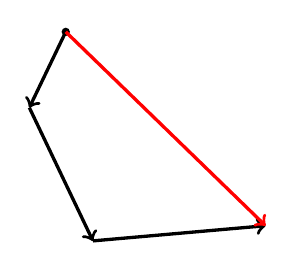
\begin{tikzpicture}[scale=0.5]
      \fill (0,0,0) circle[radius=3pt];
      \draw[->,very thick] (0,0,0) -- (1,0,5);
      \draw[->,very thick] (1,0,5) -- (3,-3,6);
      \draw[->,very thick] (3,-3,6) -- (7,-3,5);
      \draw[->,very thick,color=red] (0,0,0) -- (7,-3,5);
    \end{tikzpicture}
  \end{gather*}
  \item
  \begin{gather*}
    \vv{e} = \vv{a} - \vv{b} = \vv{a} + (-\vv{b}) \text{ (Gegenvektor von $\vv{b}$)} \\
    \vv{e} = \begin{pmatrix}1 \\ 0 \\ 5\end{pmatrix} - \begin{pmatrix}2 \\ -3 \\ 1\end{pmatrix} = \begin{pmatrix}1 \\ 0 \\ 5\end{pmatrix} + \begin{pmatrix}-2 \\ 3 \\ -1\end{pmatrix} = \begin{pmatrix}-1 \\ 3 \\ 4\end{pmatrix}
  \end{gather*}
  \begin{gather*}
    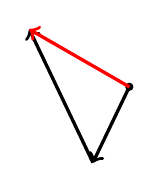
\begin{tikzpicture}[scale=0.5]
      \fill (0,0,0) circle[radius=3pt];
      \draw[->,very thick] (0,0,0) -- (1,0,5);
      \draw[->,very thick] (1,0,5) -- (-1,3,4);
      \draw[->,very thick,color=red] (0,0,0) -- (-1,3,4);
    \end{tikzpicture}
  \end{gather*}
  \item
  \begin{gather*}
    \vv{f} = 3 \cdot \vv{a} \\
    \vv{f} = 3 \cdot \begin{pmatrix}1 \\ 0 \\ 5\end{pmatrix} = \begin{pmatrix}3 \\ 0 \\ 15\end{pmatrix}
  \end{gather*}
\end{itemize}
\subsubsection{Darstellung eines Vektors durch andere Vektoren (Bsp. Verbindungsvektor)}
\begin{gather*}
  \vv{a} = \vv{OA} = \begin{pmatrix}4 \\ 4 \\ 1\end{pmatrix} \gap\gap \vv{b} = \vv{OB} = \begin{pmatrix}-1 \\ 0 \\ 3\end{pmatrix} \\
  \vv{AB} = -\vv{a} + \vv{b} = -\vv{OA} + \vv{OB} = \vv{OB} - \vv{OA} = \begin{pmatrix}-1 \\ 0 \\ 3\end{pmatrix} - \begin{pmatrix}4 \\ 4 \\ 1\end{pmatrix} = \begin{pmatrix}-5 \\ -4 \\ 2\end{pmatrix}
\end{gather*}
\begin{exercise}{279/6}
  \item [a]
  \begin{gather*}
    A(-2|2|3) \gap\gap B(5|5|5) \gap\gap C(9|6|5) \gap\gap D(2|3|3) \\
    \vv{AB} = \begin{pmatrix}7 \\ 3 \\ 2\end{pmatrix} \gap\gap \vv{DC} = \begin{pmatrix}7 \\ 3 \\ 2\end{pmatrix} \\
    \vv{AB} = \vv{DC} \gap\Rightarrow\gap \text{Parallelogramm}
  \end{gather*}
  \item [b]
  \begin{gather*}
    A(2|0|3) \gap\gap B(4|4|4) \gap\gap C(11|7|9) \gap\gap D(9|3|8) \\
    \vv{AB} = \begin{pmatrix}2 \\ 4 \\ 1\end{pmatrix} \gap\gap \vv{DC} = \begin{pmatrix}2 \\ 4 \\ 1\end{pmatrix} \\
    \vv{AB} = \vv{DC} \gap\Rightarrow\gap \text{Parallelogramm}
  \end{gather*}
  \item [c]
  \begin{gather*}
    A(2|-2|7) \gap\gap B(6|5|1) \gap\gap C(1|-1|1) \gap\gap D(8|0|8) \\
    \vv{AB} = \begin{pmatrix}4 \\ 7 \\ -6\end{pmatrix} \gap\gap \vv{DC} = \begin{pmatrix}-7 \\ -1 \\ -7\end{pmatrix} \\
    \vv{AB} \neq \vv{DC} \gap\Rightarrow\gap \text{kein Parallelogramm}
  \end{gather*}
\end{exercise}
\newpage
\begin{exercise}{279/7}
  \item [a]
  \begin{gather*}
    A(21|-11|43) \gap\gap B(3|7|-8) \gap\gap C(0|4|5) \\
  \vv{AB} = \begin{pmatrix}-18 \\ 18 \\ -51\end{pmatrix} \gap\gap \vv{BC} = \begin{pmatrix}-3 \\ -3 \\ 13\end{pmatrix} \\
  \vv{OD_1} = \vv{OA} + \vv{BC} = \begin{pmatrix}18 \\ -14 \\ 56\end{pmatrix} \\
  \vv{OD_2} = \vv{OC} + \vv{AB} = \begin{pmatrix}-18 \\ 22 \\ -46\end{pmatrix} \\
  \vv{OD_3} = \vv{OA} - \vv{BC} = \begin{pmatrix}24 \\ -8 \\ 30\end{pmatrix}
  \end{gather*}
  \begin{gather*}
    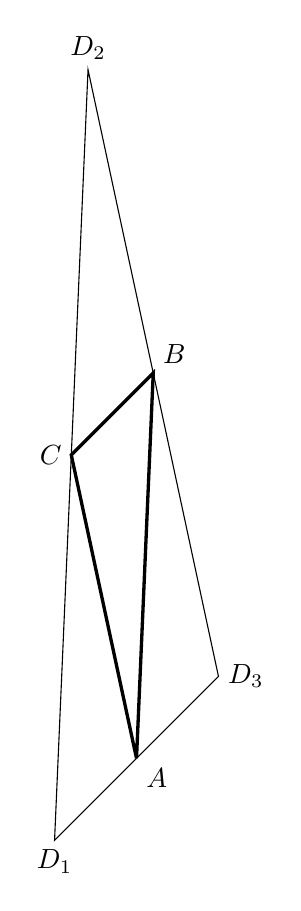
\begin{tikzpicture}[scale=0.13]
      \coordinate (A) at (21,-11,43);
      \coordinate (B) at (3,7,-8);
      \coordinate (C) at (0,4,5);
      \coordinate (D1) at (18,-14,56);
      \coordinate (D2) at (-18,22,-46);
      \coordinate (D3) at (24,-8,30);
      \node[below right] at (A) {$A$};
      \node[above right] at (B) {$B$};
      \node[left] at (C) {$C$};
      \node[below] at (D1) {$D_1$};
      \node[above] at (D2) {$D_2$};
      \node[right] at (D3) {$D_3$};
      \draw[very thick] (A) -- (B) -- (C) -- (A);
      \draw (A) -- (D1) -- (C);
      \draw (B) -- (D2) -- (C);
      \draw (A) -- (D3) -- (B);
    \end{tikzpicture}
  \end{gather*}
  \item [b]
  \begin{gather*}
    A(-75|199|-67) \gap\gap B(35|0|-81) \gap\gap C(1|2|3) \\
    \vv{AB} = \begin{pmatrix}110 \\ -199 \\ 14\end{pmatrix} \gap\gap \vv{BC} = \begin{pmatrix}-34 \\ 2 \\ 84\end{pmatrix} \\
    \vv{OD_1} = \vv{OA} + \vv{BC} = \begin{pmatrix}-109 \\ 201 \\ 17\end{pmatrix} \\
    \vv{OD_2} = \vv{OC} + \vv{AB} = \begin{pmatrix}111 \\ -197 \\ 17\end{pmatrix} \\
    \vv{OD_3} = \vv{OA} - \vv{BC} = \begin{pmatrix}-41 \\ 197 \\ -151\end{pmatrix}
  \end{gather*}
  \begin{gather*}
    \begin{tikzpicture}[scale=0.024]
      \coordinate (A) at (-75,199,-67);
      \coordinate (B) at (35,0,-81);
      \coordinate (C) at (1,2,3);
      \coordinate (D1) at (-109,201,17);
      \coordinate (D2) at (111,-197,17);
      \coordinate (D3) at (-41,197,-151);
      \node[above left] at (A) {$A$};
      \node[right] at (B) {$B$};
      \node[below left] at (C) {$C$};
      \node[left] at (D1) {$D_1$};
      \node[below right] at (D2) {$D_2$};
      \node[above right] at (D3) {$D_3$};
      \draw[very thick] (A) -- (B) -- (C) -- (A);
      \draw (A) -- (D1) -- (C);
      \draw (B) -- (D2) -- (C);
      \draw (A) -- (D3) -- (B);
    \end{tikzpicture}
  \end{gather*}
\end{exercise}
\subsection{Vektorzüge und Linearkombinationen}
(zu 279/6) \\\\
$M_1$ ... Mittelpunkt von $\overline{AB}$ \\
$M_2$ ... Mittelpunkt des Parallelogramms (mit $D_1$)
\begin{gather*}
  \vv{OM_1} = \vv{OA} + \frac{1}{2} \cdot \vv{AB} = \vv{OB} - \frac{1}{2}\vv{AB} \\
  \vv{OM_2} = \vv{OA} + \frac{1}{2} \cdot \vv{AC} = \vv{OC} - \frac{1}{2}\vv{AC}
\end{gather*}
\begin{itemize}
  \item [zu 6a]
  \begin{gather*}
    \vv{OA} = \begin{pmatrix}-2 \\ 2 \\ 3\end{pmatrix} \gap\gap \vv{OB} = \begin{pmatrix}5 \\ 5 \\ 5\end{pmatrix} \gap\gap \vv{OC} = \begin{pmatrix}9 \\ 6 \\ 5\end{pmatrix} \\
    \vv{OM_1} = \begin{pmatrix}-2 \\ 2 \\ 3\end{pmatrix} + \frac{1}{2} \cdot \begin{pmatrix}7 \\ 3 \\ 2\end{pmatrix} = \begin{pmatrix}1.5 \\ 3.5 \\ 4\end{pmatrix} \\
    \vv{OM_2} = \begin{pmatrix}-2 \\ 2 \\ 3\end{pmatrix} + \frac{1}{2} \cdot \begin{pmatrix}11 \\ 4 \\ 2\end{pmatrix} = \begin{pmatrix}3.5 \\ 4 \\ 4\end{pmatrix}
  \end{gather*}
  \item [zu 6b]
  \begin{gather*}
    \vv{OA} = \begin{pmatrix}2 \\ 0 \\ 3\end{pmatrix} \gap\gap \vv{OB} = \begin{pmatrix}4 \\ 4 \\ 4\end{pmatrix} \gap\gap \vv{OC} = \begin{pmatrix}11 \\ 7 \\ 9\end{pmatrix} \\
    \vv{OM_1} = \begin{pmatrix}2 \\ 0 \\ 3\end{pmatrix} + \frac{1}{2} \cdot \begin{pmatrix}2 \\ 4 \\ 1\end{pmatrix} = \begin{pmatrix}3 \\ 2 \\ 3.5\end{pmatrix} \\
    \vv{OM_2} = \begin{pmatrix}2 \\ 0 \\ 3\end{pmatrix} + \frac{1}{2} \cdot \begin{pmatrix}9 \\ 7 \\ 6\end{pmatrix} = \begin{pmatrix}6.5 \\ 3.5 \\ 6\end{pmatrix}
  \end{gather*}
\end{itemize}
Setze ich mehrere Vektorpfeile, mit Koeffizienten multipliziert, aneinander, so nennt man das einen Vektorzug. Die rechnerische Summe solcher Vektoren heißt Linearkombination.
\newpage
\begin{exercise}{283/5}
  \item [a]
  \begin{gather*}
    2 \cdot \begin{pmatrix}1 \\ 2\end{pmatrix} + 3 \cdot \begin{pmatrix}2 \\ 0\end{pmatrix} = \begin{pmatrix}8 \\ 4\end{pmatrix}
  \end{gather*}
  \begin{gather*}
    \begin{tikzpicture}
      \draw[->] (0,0) -- (1,2);
      \draw[->] (1,2) -- (2,4);
      \draw[->] (2,4) -- (4,4);
      \draw[->] (4,4) -- (6,4);
      \draw[->] (6,4) -- (8,4);
      \draw[->] (0,0) -- (2,0);
      \draw[->] (2,0) -- (4,0);
      \draw[->] (4,0) -- (6,0);
      \draw[->] (6,0) -- (7,2);
      \draw[->] (7,2) -- (8,4);
      \draw[->,color=red] (0,0) -- (8,4);
    \end{tikzpicture}
  \end{gather*}
  \item [b]
  \begin{gather*}
    4 \cdot \begin{pmatrix}1 \\ 1\end{pmatrix} - 2 \cdot \begin{pmatrix}1 \\ 3\end{pmatrix} = \begin{pmatrix}2 \\ -2\end{pmatrix}
  \end{gather*}
  \begin{gather*}
    \begin{tikzpicture}
      \draw[->] (0,0) -- (1,1);
      \draw[->] (1,1) -- (2,2);
      \draw[->] (2,2) -- (3,3);
      \draw[->] (3,3) -- (4,4);
      \draw[->] (4,4) -- (3,1);
      \draw[->] (3,1) -- (2,-2);
      \draw[->] (0,0) -- (-1,-3);
      \draw[->] (-1,-3) -- (-2,-6);
      \draw[->] (-2,-6) -- (-1,-5);
      \draw[->] (-1,-5) -- (0,-4);
      \draw[->] (0,-4) -- (1,-3);
      \draw[->] (1,-3) -- (2,-2);
      \draw[->,color=red] (0,0) -- (2,-2);
    \end{tikzpicture}
  \end{gather*}
  \item [c]
  \begin{gather*}
  3 \cdot \begin{pmatrix}-1 \\ -2\end{pmatrix} + 2 \cdot \begin{pmatrix}1 \\ -3\end{pmatrix} = \begin{pmatrix}-1 \\ -12\end{pmatrix}
  \end{gather*}
  \begin{gather*}
    \begin{tikzpicture}
      \draw[->] (0,0) -- (-1,-2);
      \draw[->] (-1,-2) -- (-2,-4);
      \draw[->] (-2,-4) -- (-3,-6);
      \draw[->] (-3,-6) -- (-2,-9);
      \draw[->] (-2,-9) -- (-1,-12);
      \draw[->] (0,0) -- (1,-3);
      \draw[->] (1,-3) -- (2,-6);
      \draw[->] (2,-6) -- (1,-8);
      \draw[->] (1,-8) -- (0,-10);
      \draw[->] (0,-10) -- (-1,-12);
      \draw[->,color=red] (0,0) -- (-1,-12);
    \end{tikzpicture}
  \end{gather*}
\end{exercise}
\begin{exercise}{283/7}
  \item [d]
  \begin{gather*}
    \begin{pmatrix}5 \\ 6 \\ 7\end{pmatrix} + (-1) \cdot \begin{pmatrix}0 \\ 2 \\ 4\end{pmatrix} = \begin{pmatrix}5 \\ 4 \\ 3\end{pmatrix}
  \end{gather*}
  \item [e]
  \begin{gather*}
    3 \cdot \begin{pmatrix}-1 \\ 4 \\ 2\end{pmatrix} - 2 \cdot \begin{pmatrix}-2 \\ 4 \\ 1\end{pmatrix} + 3 \cdot \begin{pmatrix}-1 \\ 4 \\ 2\end{pmatrix} = \begin{pmatrix}-2 \\ 16 \\ 10\end{pmatrix}
  \end{gather*}
  \item [f]
  \begin{gather*}
    4 \cdot \begin{pmatrix}0.5 \\ 3 \\ 1\end{pmatrix} + 2 \cdot \begin{pmatrix}1 \\ 6 \\ 2\end{pmatrix} + 3 \cdot \begin{pmatrix}0.8 \\ 2 \\ 3\end{pmatrix} = \begin{pmatrix}6.4 \\ 30 \\ 17\end{pmatrix}
  \end{gather*}
\end{exercise}
\begin{exercise}{284/11}
  \item [f] $-(\vv{u} - \vv{v}) = \vv{v} - \vv{u}$
  \item [g] $2(2\vv{a} + 4\vv{b}) = 4\vv{a} + 8\vv{b}$
  \item [h] $-4(\vv{a} - \vv{b}) - \vv{b} + \vv{a} = 3\vv{a} - 3\vv{b}$
  \item [i] $3(\vv{a} + 2(\vv{a} + \vv{b})) = 9\vv{a} + 6\vv{b}$
  \item [j] $6(\vv{a} - \vv{b}) + 4(\vv{a} + \vv{b}) = 10\vv{a} - 2\vv{b}$
  \item [k] $7\vv{u} + 5(\vv{u} - 2(\vv{u} + \vv{v})) = 2\vv{u} - 10\vv{v}$
\end{exercise}
\begin{exercise}{284/12}
  \item [a] $\vv{AG} = \vv{a} + \vv{b} + \vv{c}$
  \item [b] $\vv{BH} = -\vv{a} + \vv{b} + \vv{c}$
  \item [c] $\vv{EC} = \vv{a} + \vv{b} - \vv{c}$
  \item [d] $\vv{ME} = -\frac{1}{2}\vv{a} - \frac{1}{2}\vv{b} + \vv{c}$
\end{exercise}
\section{Geraden in $\mathbb{R}^3$}
\begin{gather*}
  \begin{tikzpicture}
    \coordinate (O) at (0,0,0);
    \coordinate (A) at (-1,0,3);
    \coordinate (B) at (3,0,3);
    \coordinate (S1) at (1,0,3);
    \coordinate (S2) at (0,0,3);
    \coordinate (S3) at (2,0,3);
    \coordinate (S4) at (5,0,3);
    \coordinate (S5) at (-2,0,3);
    \node[above] at (O) {$O$};
    \node[above] at (A) {$A$};
    \node[above] at (B) {$B$};
    \node[above] at (S1) {$S_1$};
    \node[above] at (S2) {$S_2$};
    \node[above] at (S3) {$S_3$};
    \node[above] at (S4) {$S_4$};
    \node[above] at (S5) {$S_5$};
    \fill (O) circle[radius=1pt];
    \fill (A) circle[radius=1pt];
    \fill (B) circle[radius=1pt];
    \fill (S1) circle[radius=1pt];
    \fill (S2) circle[radius=1pt];
    \fill (S3) circle[radius=1pt];
    \fill (S4) circle[radius=1pt];
    \fill (S5) circle[radius=1pt];
    \draw (A) -- (B);
  \end{tikzpicture}
\end{gather*}
\begin{gather*}
  \vv{OS_1} = \vv{OA} + \frac{1}{2}\vv{AB} \\
  \vv{OS_2} = \vv{OA} + \frac{1}{4}\vv{AB} \\
  \vv{OS_3} = \vv{OA} + \frac{3}{4}\vv{AB} \\
  \vv{OS_4} = \vv{OA} + \frac{3}{2}\vv{AB} = \vv{OB} + \frac{1}{2}\vv{AB} \\
  \vv{OS_5} = \vv{OA} - \frac{1}{4}\vv{AB}
\end{gather*}
Gerade durch die Punkte $A$ und $B$:
\begin{gather*}
  g: \vv{x} = \vv{OA} + s \cdot \vv{AB} \gap\gap s \in \mathbb{R}
\end{gather*}
Parametergleichung einer Geraden $g$:
\begin{itemize}
  \item [$g$] Name der Geraden
  \item [$\vv{x}$] Ortsvektor eines unbestimmten Punktes
  \item [$\vv{OA}$] Ortsvektor eines bestimmten Punktes $A$ (heißt auch Stützvektor)
  \item [$s$] Parameter $s \in \mathbb{R}$ \\
  Beim Durchlaufen aller Zahlen von $\mathbb{R}$ werden nacheinander alle Punkte der Geraden $g$ dargestellt
  \item [$\vv{AB}$] Richtungsvektor von $g$ gibt die Richtung von $g$ an
\end{itemize}
\begin{gather*}
  h: \vv{x} = \vv{a} + r \cdot \vv{b} \\
  h: \vv{x} = \begin{pmatrix}1 \\ 0 \\ 2\end{pmatrix} + r \cdot \begin{pmatrix}-3 \\ 5 \\ 2\end{pmatrix} \\\\
  \text{Beispiele für Punkte auf $h$} \\
  \vv{OP_1} = \begin{pmatrix}1 \\ 0 \\ 2\end{pmatrix} \gap\gap r = 0 \\
  \vv{OP_2} = \begin{pmatrix}-2 \\ 5 \\ 4\end{pmatrix} \gap\gap r = 1 \\
  \vv{OP_3} = \begin{pmatrix}-5 \\ 10 \\ 6\end{pmatrix} \gap\gap r = 2 \\
  \vv{OP_4} = \begin{pmatrix}4 \\ -5 \\ 0\end{pmatrix} \gap\gap r = -1
\end{gather*}
\begin{gather*}
  \vv{OQ} = \begin{pmatrix}3 \\ 7 \\ -1\end{pmatrix} \in h \\
  \begin{pmatrix}3 \\ 7 \\ -1\end{pmatrix} = \begin{pmatrix}1 \\ 0 \\ 2\end{pmatrix} + r \cdot \begin{pmatrix}-3 \\ 5 \\ 2\end{pmatrix} \\
  \text{gibt es ein $r$, das alle 3 Gleichungen löst?} \\
  3 = 1 - 3r \gap\Rightarrow\gap r = -\frac{2}{3} \\
  7 = 5r \gap\Rightarrow\gap r = \frac{7}{5} \\
  -1 = 2 + 2r \gap\Rightarrow\gap r = -\frac{3}{2} \\
  \Rightarrow\gap Q \notin h
\end{gather*}
\begin{exercise}{287/2}
  \item [a]
  \begin{gather*}
    A(1|2|2) \gap\gap B(5|-4|7) \\
    g: \vv{x} = \vv{OA} + s \cdot \vv{AB} = \begin{pmatrix}1 \\ 2 \\ 2\end{pmatrix} + s \cdot \begin{pmatrix}4 \\ -6 \\ 5\end{pmatrix} \\
    g: \vv{x} = \vv{OB} + s \cdot \vv{AB} = \begin{pmatrix}5 \\ -4 \\ 7\end{pmatrix} + s \cdot \begin{pmatrix}4 \\ -6 \\ 5\end{pmatrix}
  \end{gather*}
  \item [b]
  \begin{gather*}
    A(-3|-2|9) \gap\gap B(0|0|3) \\
    g: \vv{x} = \vv{OA} + s \cdot \vv{AB} = \begin{pmatrix}-3 \\ -2 \\ 9\end{pmatrix} + s \cdot \begin{pmatrix}3 \\ 2 \\ -6\end{pmatrix} \\
    g: \vv{x} = \vv{OB} + s \cdot \vv{AB} = \begin{pmatrix}0 \\ 0 \\ 3\end{pmatrix} + s \cdot \begin{pmatrix}3 \\ 2 \\ -6\end{pmatrix}
  \end{gather*}
  \item [c]
  \begin{gather*}
    A(7|-2|7) \gap\gap B(1|1|1) \\
    g: \vv{x} = \vv{OA} + s \cdot \vv{AB} = \begin{pmatrix}7 \\ -2 \\ 7\end{pmatrix} + s \cdot \begin{pmatrix}-6 \\ 3 \\ -6\end{pmatrix} \\
    g: \vv{x} = \vv{OB} + s \cdot \vv{AB} = \begin{pmatrix}1 \\ 1 \\ 1\end{pmatrix} + s \cdot \begin{pmatrix}-6 \\ 3 \\ -6\end{pmatrix}
  \end{gather*}
\end{exercise}
\begin{exercise}{287/3}
  \item [c]
  \begin{gather*}
    X(2|3|-1) \gap\gap g: \vv{x} = \begin{pmatrix}7 \\ 0 \\ 4\end{pmatrix} + t \cdot \begin{pmatrix}5 \\ -3 \\ 5\end{pmatrix} \\
    2 = 7 + t \cdot 5 \gap\Rightarrow\gap t = -1 \\
    3 = t \cdot -3 \gap\Rightarrow\gap t = -1 \\
    -1 = 4 + t \cdot 5 \gap\Rightarrow\gap t = -1 \\
    \Rightarrow\gap X \in g
  \end{gather*}
  \item [d]
  \begin{gather*}
    X(2|-1|-1) \gap\gap g: \vv{x} = \begin{pmatrix}1 \\ 0 \\ 1\end{pmatrix} + t \cdot \begin{pmatrix}1 \\ 3 \\ 3\end{pmatrix} \\
    2 = 1 + t \gap\Rightarrow\gap t = 1 \\
    -1 = t \cdot 3 \gap\Rightarrow\gap t = -\frac{1}{3} \\
    \Rightarrow\gap X \notin g
  \end{gather*}
\end{exercise}
\begin{exercise}{288/12}
  \item [a]
  \begin{itemize}
    \item [$g$]
    \begin{gather*}
      P_1(2|9|0) \gap\gap P_2(-4|1|0) \gap\gap g: \vv{x} = \begin{pmatrix}2 \\ 9 \\ 0\end{pmatrix} + t \cdot \begin{pmatrix}3 \\ 4 \\ 0\end{pmatrix}
    \end{gather*}
    \item [$h$]
    \begin{gather*}
      H(-4|1|3) \gap\gap P(2|5|-3) \gap\gap h: \vv{x} = \begin{pmatrix}-4 \\ 1 \\ 3\end{pmatrix} + t \cdot \begin{pmatrix}3 \\ 2 \\ -3\end{pmatrix}
    \end{gather*}
    \item [$i$]
    \begin{gather*}
      P_1(-4|5|3) \gap\gap P_2(-4|9|0) \gap\gap i: \vv{x} = \begin{pmatrix}-4 \\ 5 \\ 3\end{pmatrix} + t \cdot \begin{pmatrix}0 \\ 4 \\ -3\end{pmatrix}
    \end{gather*}
    \item [$j$]
    \begin{gather*}
      P_1(-1|1|0) \gap\gap P_2(-1|5|3) \gap\gap j: \vv{x} = \begin{pmatrix}-1 \\ 1 \\ 0\end{pmatrix} + t \cdot \begin{pmatrix}0 \\ 4 \\ 3\end{pmatrix}
    \end{gather*}
  \end{itemize}
  \item [b]
  \begin{itemize}
    \item [$g$]
    \begin{gather*}
      C(-8|11|0) \gap\gap P(-2|5|3) \gap\gap g: \vv{x} = \begin{pmatrix}-8 \\ 11 \\ 0\end{pmatrix} + t \cdot \begin{pmatrix}2 \\ -2 \\ 1\end{pmatrix}
    \end{gather*}
    \item [$h$]
    \begin{gather*}
      P_1(-2|5|3) \gap\gap P_2(-6|9|3) \gap\gap h: \vv{x} = \begin{pmatrix}-2 \\ 5 \\ 3\end{pmatrix} + t \cdot \begin{pmatrix}-2 \\ 2 \\ 0\end{pmatrix}
    \end{gather*}
    \item [$i$]
    \begin{gather*}
      B(0|11|0) \gap\gap P(-6|5|3) \gap\gap i: \vv{x} = \begin{pmatrix}0 \\ 11 \\ 0\end{pmatrix} + t \cdot \begin{pmatrix}-2 \\ -2 \\ 1\end{pmatrix}
    \end{gather*}
    \item [$j$]
    \begin{gather*}
      M(-4|7|0) \gap\gap P(-6|5|3) \gap\gap j: \vv{x} = \begin{pmatrix}-4 \\ 7 \\ 0\end{pmatrix} + t \cdot \begin{pmatrix}-2 \\ -2 \\ 3\end{pmatrix}
    \end{gather*}
  \end{itemize}
\end{exercise}
\subsection{Kollinearität}
\begin{gather*}
  g: \vv{x} = \vv{a} + t \cdot \vv{b} \gap\gap t \in \mathbb{R} \\
  \text{für $\vv{b}$ gilt: $\vv{b}$ kann durch $\vv{b}' = s \cdot \vv{b}$ ersetzt werden} \gap\gap s \in \mathbb{R} \gap s \neq 0 \\
  \vv{b}' \parallel \vv{b} \gap\gap \text{$\vv{b}'$ und $\vv{b}$ sind kollinear}
\end{gather*}
Sonderfall: Gerade durch $O$
\begin{gather*}
  \text{z. B. } g: \vv{x} = t \cdot \begin{pmatrix}1 \\ 3 \\ 5\end{pmatrix} = \begin{pmatrix}-2 \\ -6 \\ -10\end{pmatrix} + s \cdot \begin{pmatrix}1 \\ 3 \\ 5\end{pmatrix} \\
  \text{hier ist $\vv{a} \parallel \vv{b}$, d. h. $\vv{a}$ und $\vv{b}$ sind kollinear ($\vv{a} = -2 \cdot \vv{b}$)}
\end{gather*}
\subsection{Lage zweier Geraden}
4 Möglichkeiten unterschiedlicher Lage:
\begin{itemize}
  \item Schnitt (Schnittpunkt)
  \item parallel
  \item identisch
  \item windschief
\end{itemize}
\subsubsection{Verfahren um festzustellen, welche Lage zwei Geraden $g$ und $h$ haben}
\begin{gather*}
  g: \vv{x} = \vv{a} + s \cdot \vv{b} \\
  h: \vv{x} = \vv{c} + t \cdot \vv{d}
\end{gather*}
\begin{gather*}
  \vv{b} \stackrel{?}{=} r \cdot \vv{d}
\end{gather*}
\begin{itemize}
  \item wahr:
  \begin{gather*}
    \vv{a} \stackrel{?}{=} \vv{c} + t \cdot \vv{d} \text{ oder } \vv{c} \stackrel{?}{=} \vv{a} + s \cdot \vv{b}
  \end{gather*}
  \begin{itemize}
    \item wenn wahr, dann sind $g$ und $h$ identisch
    \item wenn nicht wahr, dann sind $g$ und $h$ parallel
  \end{itemize}
  \newpage
  \item nicht wahr:
  \begin{gather*}
    \vv{a} + s \cdot \vv{b} = \vv{c} + t \cdot \vv{d}
  \end{gather*}
  \begin{itemize}
    \item finde ich ein $s$ und ein $t$, sodass das LGS gelöst wird, so schneiden sich $g$ und $h$ in einem Punkt $S$
    \item ansonsten sind $g$ und $h$ windschief
  \end{itemize}
\end{itemize}
\begin{exercise}{292/1}
  \item [a]
  \begin{gather*}
    g: \vv{x} = \begin{pmatrix}1 \\ 2 \\ 3\end{pmatrix} + r \cdot \begin{pmatrix}2 \\ 4 \\ 1\end{pmatrix} \\
    h: \vv{x} = \begin{pmatrix}3 \\ 6 \\ 4\end{pmatrix} + t \cdot \begin{pmatrix}4 \\ 8 \\ 2\end{pmatrix} \\\\
    \begin{pmatrix}2 \\ 4 \\ 1\end{pmatrix} = r \cdot \begin{pmatrix}4 \\ 8 \\ 2\end{pmatrix} \\
    r = 2 \\
    \Rightarrow \text{identisch oder parallel} \\\\
    \begin{pmatrix}1 \\ 2 \\ 3\end{pmatrix} = \begin{pmatrix}3 \\ 6 \\ 4\end{pmatrix} + t \cdot \begin{pmatrix}4 \\ 8 \\ 2\end{pmatrix} \\
    t = -\frac{1}{2} \\
    \Rightarrow \text{identisch}
  \end{gather*}
\end{exercise}
\newpage
\begin{exercise}{292/2}
  \item [a]
  \begin{gather*}
    g: \vv{x} = \begin{pmatrix}9 \\ 0 \\ 6\end{pmatrix} + r \cdot \begin{pmatrix}3 \\ 2 \\ 1\end{pmatrix} \\
    h: \vv{x} = \begin{pmatrix}7 \\ -2 \\ 2\end{pmatrix} + s \cdot \begin{pmatrix}1 \\ 1 \\ 2\end{pmatrix} \\\\
    \begin{pmatrix}9 \\ 0 \\ 6\end{pmatrix} + r \cdot \begin{pmatrix}3 \\ 2 \\ 1\end{pmatrix} = \begin{pmatrix}7 \\ -2 \\ 2\end{pmatrix} + s \cdot \begin{pmatrix}1 \\ 1 \\ 2\end{pmatrix} \\\\
    9 + 3r = 7 + s \\
    2r = -2 + s \\
    6 + r = 2 + 2s \\
    \Rightarrow \gap\gap r = 0 \gap\gap s = 2 \\\\
    \vv{OS} = \begin{pmatrix}9 \\ 0 \\ 6\end{pmatrix} + 0 \cdot \begin{pmatrix}3 \\ 2 \\ 1\end{pmatrix} = \begin{pmatrix}7 \\ -2 \\ 2\end{pmatrix} + 2 \cdot \begin{pmatrix}1 \\ 1 \\ 2\end{pmatrix} = \begin{pmatrix}9 \\ 0 \\ 6\end{pmatrix} \\\\
    S(9|0|6)
  \end{gather*}
\end{exercise}
\newpage
\begin{exercise}{292/4}
  \item [a]
  \begin{gather*}
    g: \vv{x} = \begin{pmatrix}5 \\ 0 \\ 1\end{pmatrix} + t \cdot \begin{pmatrix}2 \\ 1 \\ -1\end{pmatrix} \\
    h: \vv{x} = \begin{pmatrix}7 \\ 1 \\ 2\end{pmatrix} + t \cdot \begin{pmatrix}-6 \\ -3 \\ 3\end{pmatrix} \\\\
    \begin{pmatrix}2 \\ 1 \\ -1\end{pmatrix} = r \cdot \begin{pmatrix}-6 \\ -3 \\ 3\end{pmatrix} \\
    r = -3 \\
    \Rightarrow \text{identisch oder parallel} \\\\
    \begin{pmatrix}5 \\ 0 \\ 1\end{pmatrix} = \begin{pmatrix}7 \\ 1 \\ 2\end{pmatrix} + t \cdot \begin{pmatrix}-6 \\ -3 \\ 3\end{pmatrix} \\
    5 = 7 + t \cdot (-6) \gap\Rightarrow\gap t = \frac{1}{3} \\
    0 = 1 + t \cdot (-3) \gap\Rightarrow\gap t = \frac{1}{3} \\
    1 = 2 + t \cdot 3 \gap\Rightarrow\gap t = -\frac{1}{3} \\
    \Rightarrow \text{parallel}
  \end{gather*}
  \item [b]
  \begin{gather*}
    g: \vv{x} = t \cdot \begin{pmatrix}2 \\ 0 \\ 1\end{pmatrix} \\
    h: \vv{x} = \begin{pmatrix}2 \\ 3 \\ 4\end{pmatrix} + t \cdot \begin{pmatrix}0 \\ 1 \\ -1\end{pmatrix} \\\\
    \begin{pmatrix}2 \\ 0 \\ 1\end{pmatrix} \neq r \cdot \begin{pmatrix}0 \\ 1 \\ -1\end{pmatrix} \\
    \Rightarrow \text{nicht parallel} \\\\
    t_g \cdot \begin{pmatrix}2 \\ 0 \\ 1\end{pmatrix} = \begin{pmatrix}2 \\ 3 \\ 4\end{pmatrix} + t_h \cdot \begin{pmatrix}0 \\ 1 \\ -1\end{pmatrix} \\
    t_g \cdot 2 = 2 + t_h \cdot 0 \gap\Rightarrow\gap t_g = 1 \\
    t_g \cdot 0 = 3 + t_h \cdot 1 \gap\Rightarrow\gap t_h = -1 \\
    t_g \cdot 1 \neq 4 + t_h \cdot (-1) \\
    \Rightarrow \text{windschief}
  \end{gather*}
\end{exercise}
\begin{exercise}{293/8}
  \item [b]
  \begin{gather*}
    g: \vv{x} = \begin{pmatrix}2 \\ 2 \\ 1\end{pmatrix} + t \cdot \begin{pmatrix}1 \\ 2 \\ 0\end{pmatrix} \\
    h: \vv{x} = \begin{pmatrix}2 \\ 2 \\ 1\end{pmatrix} + t \cdot \begin{pmatrix}1 \\ 2 \\ 3\end{pmatrix} \\
    i: \vv{x} = t \cdot \begin{pmatrix}1 \\ 2 \\ 0\end{pmatrix} \\
    j: \vv{x} = t \cdot \begin{pmatrix}1 \\ 2 \\ 3\end{pmatrix}
  \end{gather*}
\end{exercise}
\subsection{Parameterpunkte und -geraden}
\begin{gather*}
  \vv{OA_b} = \begin{pmatrix}1 \\ 5 \\ b\end{pmatrix} = \begin{pmatrix}1 + b \cdot 0 \\ 5 + b \cdot 0 \\ 0 + b \cdot 1\end{pmatrix} = \begin{pmatrix}1 \\ 5 \\ 0\end{pmatrix} + b \cdot \begin{pmatrix}0 \\ 0 \\ 1\end{pmatrix} \\
  \vv{OC_d} = \begin{pmatrix}2d \\ 1 - 5d \\ 7\end{pmatrix} = \begin{pmatrix}0 + d \cdot 2 \\ 1 + d \cdot (-5) \\ 7 + d \cdot 0\end{pmatrix} = \begin{pmatrix}0 \\ 1 \\ 7\end{pmatrix} + d \cdot \begin{pmatrix}2 \\ -5 \\ 0\end{pmatrix}
\end{gather*}
\begin{gather*}
  g_a: \vv{x} = \begin{pmatrix}2 \\ a \\ 5\end{pmatrix} + r \begin{pmatrix}1 \\ 2 \\ 0\end{pmatrix} = \begin{pmatrix}2 \\ 0 \\ 5\end{pmatrix} + a \cdot \begin{pmatrix}0 \\ 1 \\ 0\end{pmatrix} + r \cdot \begin{pmatrix}1 \\ 2 \\ 0\end{pmatrix}
\end{gather*}
\begin{exercise}{293/10}
  \item [a]
  \begin{gather*}
    g_a: \vv{x} = \begin{pmatrix}3 \\ a \\ 3\end{pmatrix} + r \cdot \begin{pmatrix}-1 \\ 5 \\ 7\end{pmatrix} \gap\gap\gap h_a: \vv{x} = \begin{pmatrix}1 \\ 0 \\ a\end{pmatrix} + s \cdot \begin{pmatrix}2 \\ -22 \\ -29\end{pmatrix} \\\\
    \begin{pmatrix}-1 \\ 5 \\ 7\end{pmatrix} \neq t \cdot \begin{pmatrix}2 \\ -22 \\ -29\end{pmatrix} \\
    \Rightarrow \text{nicht parallel} \\\\
    \begin{pmatrix}3 \\ a \\ 3\end{pmatrix} + r \cdot \begin{pmatrix}-1 \\ 5 \\ 7\end{pmatrix} = \begin{pmatrix}1 \\ 0 \\ a\end{pmatrix} + s \cdot \begin{pmatrix}2 \\ -22 \\ -29\end{pmatrix} \\
    3 - r = 1 + 2s \\
    a + 5r = -22s \\
    3 + 7r = a - 29s \\
    a = 2 \gap\gap r = 4 \gap\gap s = -1 \\\\
    \vv{OS} = \begin{pmatrix}3 \\ 2 \\ 3\end{pmatrix} + 4 \cdot \begin{pmatrix}-1 \\ 5 \\ 7\end{pmatrix} = \begin{pmatrix}-1 \\ 22 \\ 31\end{pmatrix}
  \end{gather*}
  \item [b]
  \begin{gather*}
    g_a: \vv{x} = \begin{pmatrix}3 \\ 2 \\ a\end{pmatrix} + r \cdot \begin{pmatrix}10 \\ 7 \\ 0\end{pmatrix} \gap\gap\gap h_a: \vv{x} = \begin{pmatrix}a \\ -1 \\ 3\end{pmatrix} + s \cdot \begin{pmatrix}6 \\ 2 \\ -1\end{pmatrix} \\\\
    \begin{pmatrix}10 \\ 7 \\ 0\end{pmatrix} \neq t \cdot \begin{pmatrix}6 \\ 2 \\ -1\end{pmatrix} \\
    \Rightarrow \text{nicht parallel} \\\\
    \begin{pmatrix}3 \\ 2 \\ a\end{pmatrix} + r \cdot \begin{pmatrix}10 \\ 7 \\ 0\end{pmatrix} = \begin{pmatrix}a \\ -1 \\ 3\end{pmatrix} + s \cdot \begin{pmatrix}6 \\ 2 \\ -1\end{pmatrix} \\
    3 + 10r = a + 6s \\
    2 + 7r = -1 + 2s \\
    a = 3 - s \\
    a = 5 \gap\gap r = -1 \gap\gap s = -2 \\\\
    \vv{OS} = \begin{pmatrix}3 \\ 2 \\ 5\end{pmatrix} - \begin{pmatrix}10 \\ 7 \\ 0\end{pmatrix} = \begin{pmatrix}-7 \\ -5 \\ 5\end{pmatrix}
  \end{gather*}
\end{exercise}
\begin{exercise}{293/16}
  \begin{gather*}
    G = 10cm^2 \gap\gap h = 15cm \\
    V_Z = G \cdot h = 150cm^3 \\
    V_K = \frac{1}{3} \cdot G \cdot h = 50cm^3 \\
    V_Z - V_K = 100cm^3 = 0.1L
  \end{gather*}
\end{exercise}
\section{Abstand zweier Punkte, Vektorlänge, Streckenlänge}
\begin{gather*}
  \text{Bsp. } g: \vv{x} = \begin{pmatrix}1 \\ 2 \\ 3\end{pmatrix} + r \cdot \begin{pmatrix}2 \\ -1 \\ 0\end{pmatrix} \gap\gap r \in \mathbb{R}: \left[2;5\right]
\end{gather*}
\begin{gather*}
  \begin{tikzpicture}[scale=0.5]
    \coordinate (O) at (0,0,0);
    \coordinate (A) at (1,2,3);
    \coordinate (C) at (5,0,3);
    \coordinate (D) at (11,-3,3);
    \node[below] at (O) {$O$};
    \node[above right] at (A) {$A$};
    \node[above right] at (C) {$C$};
    \node[above right] at (D) {$D$};
    \fill (O) circle[radius=2pt];
    \fill (A) circle[radius=2pt];
    \draw[->] (O) -- (A);
    \draw (-3,4,3) -- (15,-5,3);
    \draw[red,very thick] (C) -- (D);
  \end{tikzpicture}
\end{gather*}
\begin{gather*}
  \vv{OC} = \begin{pmatrix}5 \\ 0 \\ 3\end{pmatrix} \gap\gap \vv{OD} = \begin{pmatrix}11 \\ -3 \\ 3\end{pmatrix} \\
  |\overline{CD}| = |\vv{CD}| = \text{Abstand } C \leftrightarrow D \\
  \vv{CD} = \begin{pmatrix}6 \\ -3 \\ 0\end{pmatrix}
\end{gather*}
\begin{gather*}
  \textbf{Seitenlängen des Segels (Bsp. S. 294)} \\
  \text{unten: } 4m \\
  \text{links: } \sqrt{(5m)^2 + (3m)^2} \gap\text{(Satz des Pythagoras)} \\
  \text{rechts: } \sqrt{(\sqrt{34}m)^2 + (4m)^2} = \sqrt{(5m)^2 + (3m)^2 + (4m)^2}
\end{gather*}
\begin{gather*}
  |\vv{CD}| = \sqrt{6^2 + (-3)^2 + 0^2} = \sqrt{45} \approx 6.71LE
\end{gather*}
Die Länge eines Vektors $\begin{pmatrix}a \\ b \\ c\end{pmatrix}$ ist $\Biggl|\begin{pmatrix}a \\ b \\ c\end{pmatrix}\Biggl| = \sqrt{a^2 + b^2 + c^2}$
\begin{exercise}{297/2}
  \item [a]
  \begin{gather*}
    A(0|0|0) \gap\gap B(2|3|-1) \\
    \vv{AB} = \begin{pmatrix}2 \\ 3 \\ -1\end{pmatrix} \\
    |\vv{AB}| = \sqrt{2^2 + 3^2 + (-1)^2} = \sqrt{14} \approx 3.74LE
  \end{gather*}
  \item [b]
  \begin{gather*}
    A(2|2|-2) \gap\gap B(0|-1|5) \\
    \vv{AB} = \begin{pmatrix}-2 \\ -3 \\ 7\end{pmatrix} \\
    |\vv{AB}| = \sqrt{(-2)^2 + (-3)^2 + 7^2} = \sqrt{62} \approx 7.87LE
  \end{gather*}
  \item [c]
  \begin{gather*}
    A(1|5|6) \gap\gap B(1|6|7) \\
    \vv{AB} = \begin{pmatrix}0 \\ 1 \\ 1\end{pmatrix} \\
    |\vv{AB}| = \sqrt{0^2 + 1^2 + 1^2} = \sqrt{2} \approx 1.41LE
  \end{gather*}
\end{exercise}
\subsection{Einheitsvektor}
Ein Einheitsvektor hat die Länge $1LE$ \\
Einheitsvektor zu z. B. $\vv{a} = \begin{pmatrix}2 \\ 5 \\ 1\end{pmatrix} \gap\gap |\vv{a}| = \sqrt{30}$
\begin{gather*}
  \vv{a_0} = \frac{1}{\sqrt{30}} \cdot \begin{pmatrix}2 \\ 5 \\ 1\end{pmatrix}
\end{gather*}
\begin{exercise}{297/8}
  \item [a]
  \begin{gather*}
    A(1|-2|2) \gap\gap B(3|2|1) \gap\gap C(3|0|3) \\
    \vv{AB} = \begin{pmatrix}2 \\ 4 \\ -1\end{pmatrix} \gap\gap |\vv{AB}| = \sqrt{2^2 + 4^2 + (-1)^2} = \sqrt{21} \\
    \vv{AC} = \begin{pmatrix}2 \\ 2 \\ 1\end{pmatrix} \gap\gap |\vv{AC}| = \sqrt{2^2 + 2^2 + 1^2} = \sqrt{9} \\
    \vv{BC} = \begin{pmatrix}0 \\ -2 \\ 2\end{pmatrix} \gap\gap |\vv{BC}| = \sqrt{0^2 + (-2)^2 + 2^2} = \sqrt{8} \\
    |\vv{AB}| \neq |\vv{AC}| \neq |\vv{BC}| \gap\Rightarrow\text{nicht gleichschenklig}
  \end{gather*}
  \item [b]
  \begin{gather*}
    A(7|0|-1) \gap\gap B(5|-3|-1) \gap\gap C(4|0|1) \\
    \vv{AB} = \begin{pmatrix}-2 \\ -3 \\ 0\end{pmatrix} \gap\gap |\vv{AB}| = \sqrt{(-2)^2 + (-3)^2 + 0^2} = \sqrt{13} \\
    \vv{AC} = \begin{pmatrix}-3 \\ 0 \\ 2\end{pmatrix} \gap\gap |\vv{AC}| = \sqrt{(-3)^2 + 0^2 + 2^2} = \sqrt{13} \\
    \vv{BC} = \begin{pmatrix}-1 \\ 3 \\ 2\end{pmatrix} \gap\gap |\vv{BC}| = \sqrt{(-1)^2 + 3^2 + 2^2} = \sqrt{14} \\
    |\vv{AB}| = |\vv{AC}| \gap\Rightarrow\text{gleichschenklig}
  \end{gather*}
\end{exercise}
\begin{exercise}{297/9}
  \item [a]
  \begin{gather*}
    A(4|2|-1) \gap\gap B(10|-8|9) \gap\gap C(4|0|1) \\
    \vv{OM_a} = \vv{OB} + \frac{1}{2} \cdot \vv{BC} = \begin{pmatrix}10 \\ -8 \\ 9\end{pmatrix} + \frac{1}{2} \cdot \begin{pmatrix}-6 \\ 8 \\ -8\end{pmatrix} = \begin{pmatrix}7 \\ -4 \\ 5\end{pmatrix} \\
    \vv{OM_b} = \vv{OC} + \frac{1}{2} \cdot \vv{CA} = \begin{pmatrix}4 \\ 0 \\ 1\end{pmatrix} + \frac{1}{2} \cdot \begin{pmatrix}0 \\ 2 \\ -2\end{pmatrix} = \begin{pmatrix}4 \\ 1 \\ 0\end{pmatrix} \\
    \vv{OM_c} = \vv{OA} + \frac{1}{2} \cdot \vv{AB} = \begin{pmatrix}4 \\ 2 \\ -1\end{pmatrix} + \frac{1}{2} \cdot \begin{pmatrix}6 \\ -10 \\ 10\end{pmatrix} = \begin{pmatrix}7 \\ -3 \\ 4\end{pmatrix} \\
    |\vv{AM_a}| = \Biggl|\begin{pmatrix}3 \\ -6 \\ 6\end{pmatrix}\Biggl| = \sqrt{3^2 + (-6)^2 + 6^2} = \sqrt{81} = 9 \\
    |\vv{BM_b}| = \Biggl|\begin{pmatrix}-6 \\ 9 \\ -9\end{pmatrix}\Biggl| = \sqrt{(-6)^2 + 9^2 + (-9)^2} = \sqrt{198} \approx 14.07 \\
    |\vv{CM_c}| = \Biggl|\begin{pmatrix}3 \\ -3 \\ 3\end{pmatrix}\Biggl| = \sqrt{3^2 + (-3)^2 + 3^2} = \sqrt{27} \approx 5.20
  \end{gather*}
  \item [b]
  \begin{gather*}
    A(1|2|-1) \gap\gap B(-1|10|15) \gap\gap C(9|6|-5) \\
    \vv{OM_a} = \vv{OB} + \frac{1}{2} \cdot \vv{BC} = \begin{pmatrix}-1 \\ 10 \\ 15\end{pmatrix} + \frac{1}{2} \cdot \begin{pmatrix}10 \\ -4 \\ -20\end{pmatrix} = \begin{pmatrix}4 \\ 8 \\ 5\end{pmatrix} \\
    \vv{OM_b} = \vv{OC} + \frac{1}{2} \cdot \vv{CA} = \begin{pmatrix}9 \\ 6 \\ -5\end{pmatrix} + \frac{1}{2} \cdot \begin{pmatrix}-8 \\ -4 \\ 4\end{pmatrix} = \begin{pmatrix}5 \\ 4 \\ -3\end{pmatrix} \\
    \vv{OM_c} = \vv{OA} + \frac{1}{2} \cdot \vv{AB} = \begin{pmatrix}1 \\ 2 \\ -1\end{pmatrix} + \frac{1}{2} \cdot \begin{pmatrix}-2 \\ 8 \\ 16\end{pmatrix} = \begin{pmatrix}0 \\ 6 \\ 7\end{pmatrix} \\
    |\vv{AM_a}| = \Biggl|\begin{pmatrix}3 \\ 6 \\ 6\end{pmatrix}\Biggl| = \sqrt{3^2 + 6^2 + 6^2} = \sqrt{81} = 9 \\
    |\vv{BM_b}| = \Biggl|\begin{pmatrix}6 \\ -6 \\ -18\end{pmatrix}\Biggl| = \sqrt{6^2 + (-6)^2 + (-18)^2} = \sqrt{396} \approx 19.90 \\
    |\vv{CM_c}| = \Biggl|\begin{pmatrix}-9 \\ 0 \\ 12\end{pmatrix}\Biggl| = \sqrt{(-9)^2 + 0^2 + 12^2} = \sqrt{225} = 15
  \end{gather*}
  \item [c]
  \begin{gather*}
    \text{zu a} \\
    |\vv{AS}| = \frac{2}{3} \cdot |\vv{AM_a}| = 6 \\
    |\vv{BS}| = \frac{2}{3} \cdot |\vv{BM_b}| \approx 9.38 \\
    |\vv{CS}| = \frac{2}{3} \cdot |\vv{CM_c}| \approx 3.46 \\\\
    \text{zu b} \\
    |\vv{AS}| = \frac{2}{3} \cdot |\vv{AM_a}| = 6 \\
    |\vv{BS}| = \frac{2}{3} \cdot |\vv{BM_b}| \approx 13.27 \\
    |\vv{CS}| = \frac{2}{3} \cdot |\vv{CM_c}| = 10
  \end{gather*}
\end{exercise}
\section{Produkte zweier Vektoren}
\subsection{Skalarprodukt}
Beispiel aus der Physik:
\begin{figure}[H]
  \centering
  \includegraphics[width=0.55\textwidth]{/fakepath/skalarprodukt_arbeit.png}
\end{figure}
\begin{gather*}
  W = \vv{F} \cdot \vv{s} \\
  cos(\alpha) = \frac{|\vv{F_s}|}{|\vv{F}|} \gap\Rightarrow\gap |\vv{F_s}| = |\vv{F}| \cdot cos(\alpha) \gap\gap\gap \text{$\vv{F_s}$ ... $\vv{F}$ in Richtung $\vv{s}$} \\
  W = \vv{F} \cdot \vv{s} = |\vv{F}| \cdot cos(\alpha) \cdot |\vv{s}| \\\\
  \vv{a} \cdot \vv{b} = |\vv{a}| \cdot |\vv{b}| \cdot cos(\alpha) = a_1 \cdot b_1 + a_2 \cdot b_2 + a_3 \cdot b_3 \\
\end{gather*}
Beispiel:
\begin{gather*}
  \vv{a} = \begin{pmatrix}1 \\ 2 \\ 3\end{pmatrix} \gap\gap \vv{b} = \begin{pmatrix}-2 \\ 0 \\ 3\end{pmatrix} \\
  \vv{a} \cdot \vv{b} = 1 \cdot (-2) + 2 \cdot 0 + 3 \cdot 3 = 7 \\\\
  \text{Winkel zwischen $\vv{a}$ und $\vv{b}$:} \\
  7 = \Biggl|\begin{pmatrix}1 \\ 2 \\ 3\end{pmatrix}\Biggl| \cdot \Biggl|\begin{pmatrix}-2 \\ 0 \\ 3\end{pmatrix}\Biggl| \cdot cos(\alpha) = \sqrt{14} \cdot \sqrt{13} \cdot cos(\alpha) \\
  \alpha = acos(\frac{7}{\sqrt{14} \cdot \sqrt{13}}) \approx 1.025 \approx 58.73^\circ
\end{gather*}
Spezialfall:
\begin{gather*}
  \alpha = 90^\circ \\
  \Rightarrow cos(\alpha) = 0 \\
  \Rightarrow \vv{a} \cdot \vv{b} = 0 \\
  \vv{a} \perp \vv{b} \\\\
  \text{z. B. } \vv{a} = \begin{pmatrix}1 \\ -1 \\ 0\end{pmatrix} \gap\gap \vv{b} = \begin{pmatrix}3 \\ 3 \\ 5\end{pmatrix} \\
  \vv{a} \cdot \vv{b} = 1 \cdot 3 + (-1) \cdot 3 + 0 \cdot 5 = 0 \\
  \Rightarrow \vv{a} \perp \vv{b}
\end{gather*}
\begin{exercise}{321/1}
  \item [a]
  \begin{gather*}
    g: \vv{x} = \begin{pmatrix}2 \\ -2 \\ 0\end{pmatrix} + s \cdot \begin{pmatrix}-5 \\ 1 \\ 0\end{pmatrix} \gap\gap h: \vv{x} = \begin{pmatrix}5 \\ -1 \\ 0\end{pmatrix} + s \cdot \begin{pmatrix}-2 \\ 2 \\ 0\end{pmatrix} \\
    \begin{pmatrix}-5 \\ 1 \\ 0\end{pmatrix} \cdot \begin{pmatrix}-2 \\ 2 \\ 0\end{pmatrix} = 12 \\
    \Rightarrow g \notperp h
  \end{gather*}
  \item [b]
  \begin{gather*}
    g: \vv{x} = \begin{pmatrix}8 \\ 6 \\ -9\end{pmatrix} + s \cdot \begin{pmatrix}2 \\ -9 \\ -4\end{pmatrix} \gap\gap h: \vv{x} = \begin{pmatrix}0 \\ 0 \\ 7\end{pmatrix} + s \cdot \begin{pmatrix}5 \\ 2 \\ -2\end{pmatrix} \\
    \begin{pmatrix}2 \\ -9 \\ -4\end{pmatrix} \cdot \begin{pmatrix}5 \\ 2 \\ -2\end{pmatrix} = 0 \\
    \Rightarrow g \perp h
  \end{gather*}
\end{exercise}
\newpage
\begin{exercise}{zu 297/8}
  \item [a]
  \begin{gather*}
    \vv{AB} \cdot \vv{AC} = \begin{pmatrix}2 \\ 4 \\ -1\end{pmatrix} \cdot \begin{pmatrix}2 \\ 2 \\ 1\end{pmatrix} = 11 \gap\gap\gap |\vv{AB}| \cdot |\vv{AC}| = \sqrt{21} \cdot \sqrt{9} \\
    \alpha = acos(\frac{11}{3\sqrt{21}}) \approx 0.64 \approx 36.86^\circ \\
    \vv{BA} \cdot \vv{BC} = \begin{pmatrix}-2 \\ -4 \\ 1\end{pmatrix} \cdot \begin{pmatrix}0 \\ -2 \\ 2\end{pmatrix} = 10 \gap\gap\gap |\vv{BA}| \cdot |\vv{BC}| = \sqrt{21} \cdot \sqrt{8} \\
    \beta = acos(\frac{10}{\sqrt{21} \cdot \sqrt{8}}) \approx 0.69 \approx 39.51^\circ \\
    \vv{CA} \cdot \vv{CB} = \begin{pmatrix}-2 \\ -2 \\ -1\end{pmatrix} \cdot \begin{pmatrix}0 \\ 2 \\ -2\end{pmatrix} = -2 \gap\gap\gap |\vv{CA}| \cdot |\vv{CB}| = \sqrt{9} \cdot \sqrt{8} \\
    \gamma = acos(\frac{-2}{3\sqrt{8}}) \approx 1.81 \approx 103.63^\circ
  \end{gather*}
  \item [b]
  \begin{gather*}
    \vv{AB} \cdot \vv{AC} = \begin{pmatrix}-2 \\ -3 \\ 0\end{pmatrix} \cdot \begin{pmatrix}-3 \\ 0 \\ 2\end{pmatrix} = 6 \gap\gap\gap |\vv{AB}| \cdot |\vv{AC}| = \sqrt{13} \cdot \sqrt{13} \\
    \alpha = acos(\frac{6}{13}) \approx 1.09 \approx 62.51^\circ \\
    \vv{BA} \cdot \vv{BC} = \vv{CA} \cdot \vv{CB} = \begin{pmatrix}2 \\ 3 \\ 0\end{pmatrix} \cdot \begin{pmatrix}-1 \\ 3 \\ 2\end{pmatrix} = 7 \\
    |\vv{BA}| \cdot |\vv{BC}| = |\vv{CA}| \cdot |\vv{CB}| = \sqrt{13} \cdot \sqrt{14} \\
    \beta = \gamma = acos(\frac{7}{\sqrt{13} \cdot \sqrt{14}}) \approx 1.03 \approx 58.74^\circ
  \end{gather*}
\end{exercise}
\newpage
\begin{exercise}{zu 297/9}
  \item [a]
  \begin{gather*}
    \vv{AB} \cdot \vv{AC} = \begin{pmatrix}6 \\ -10 \\ 10\end{pmatrix} \cdot \begin{pmatrix}0 \\ -2 \\ 2\end{pmatrix} = 40 \gap\gap\gap |\vv{AB}| \cdot |\vv{AC}| = \sqrt{236} \cdot \sqrt{8} \\
    \alpha = acos(\frac{40}{\sqrt{236} \cdot \sqrt{8}}) \approx 0.40 \approx 22.99^\circ \\
    \vv{BA} \cdot \vv{BC} = \begin{pmatrix}-6 \\ 10 \\ -10\end{pmatrix} \cdot \begin{pmatrix}-6 \\ 8 \\ -8\end{pmatrix} = 196 \gap\gap\gap |\vv{BA}| \cdot |\vv{BC}| = \sqrt{236} \cdot \sqrt{164} \\
    \beta = acos(\frac{196}{\sqrt{236} \cdot \sqrt{164}}) \approx 0.09 \approx 4.95^\circ \\
    \vv{CA} \cdot \vv{CB} = \begin{pmatrix}0 \\ 2 \\ -2\end{pmatrix} \cdot \begin{pmatrix}6 \\ -8 \\ 8\end{pmatrix} = -32 \gap\gap\gap |\vv{CA}| \cdot |\vv{CB}| = \sqrt{8} \cdot \sqrt{164} \\
    \gamma = acos(\frac{-32}{\sqrt{8} \cdot \sqrt{164}}) \approx 2.65 \approx 152.06^\circ
  \end{gather*}
  \item [b]
  \begin{gather*}
    \vv{AB} \cdot \vv{AC} = \begin{pmatrix}-2 \\ 8 \\ 16\end{pmatrix} \cdot \begin{pmatrix}8 \\ 4 \\ -4\end{pmatrix} = -48 \gap\gap\gap |\vv{AB}| \cdot |\vv{AC}| = \sqrt{324} \cdot \sqrt{96} \\
    \alpha = acos(\frac{-48}{\sqrt{324} \cdot \sqrt{96}}) \approx 1.85 \approx 105.79^\circ \\
    \vv{BA} \cdot \vv{BC} = \begin{pmatrix}2 \\ -8 \\ -16\end{pmatrix} \cdot \begin{pmatrix}10 \\ -4 \\ -20\end{pmatrix} = 372 \gap\gap\gap |\vv{BA}| \cdot |\vv{BC}| = \sqrt{324} \cdot \sqrt{516} \\
    \beta = acos(\frac{372}{\sqrt{324} \cdot \sqrt{516}}) \approx 0.43 \approx 24.52^\circ \\
    \vv{CA} \cdot \vv{CB} = \begin{pmatrix}-8 \\ -4 \\ 4\end{pmatrix} \cdot \begin{pmatrix}-10 \\ 4 \\ 20\end{pmatrix} = 144 \gap\gap\gap |\vv{CA}| \cdot |\vv{CB}| = \sqrt{96} \cdot \sqrt{516} \\
    \gamma = acos(\frac{144}{\sqrt{96} \cdot \sqrt{516}}) \approx 0.87 \approx 49.68^\circ
  \end{gather*}
\end{exercise}

\end{document}
